\documentclass[11pt,a4paper,twoside]{book}

% Paquete de la plantilla (oculto en config/)
\usepackage{config/TeXiS/TeXiS}

% Mis paquetes
% MY LIBS
\usepackage{tabularx,adjustbox,booktabs}
\usepackage{xcolor}
\usepackage{tcolorbox}
\usepackage{footnote}
\usepackage{minitoc}
\usepackage{titletoc}

% BUILDABILITY
\usepackage{algorithmic}
\usepackage{graphicx}
\usepackage{textcomp}
\usepackage{xcolor}
\usepackage{hyperref}
\hypersetup{
    colorlinks,
    linkcolor={blue},
    citecolor={blue},
    urlcolor={blue}
}
\usepackage{zref-totpages}
\usepackage[flushleft]{threeparttable}
\usepackage{listings}
\usepackage{paralist}
\usepackage{hhline}
\usepackage[strings]{underscore}
\lstset
{ %Formatting for code in appendix
	basicstyle=\fontsize{7}{11}\ttfamily,
	escapeinside={<@}{@>},
	showstringspaces=false,
	tabsize=1,
	breaklines=true,
	breakatwhitespace=false
}
\usepackage{enumerate}
\usepackage{soul}
\usepackage{caption}

\newcommand\setrow[1]{\gdef\rowmac{#1}#1\ignorespaces}
\newcommand\clearrow{\global\let\rowmac\relax}
\clearrow

% BUG HUNTER

\usepackage{pifont}
\usepackage{paralist}
\usepackage{booktabs}
\usepackage{tabularx}
\usepackage{multirow}
\usepackage{hyperref}
\usepackage{amssymb}
\usepackage[normalem]{ulem}
\usepackage[linesnumbered,ruled]{algorithm2e}
  \SetKwComment{Comment}{/* }{ */}
  \SetAlFnt{\scriptsize\sf}
  \SetKw{And}{\textbf{ and }}
\usepackage{tikz}
\usetikzlibrary{arrows.meta, automata,positioning}
\tikzset{%
	large/.style = {
		minimum width=8cm,
		rectangle, draw=black,
	},
	base/.style = {
		rectangle, draw=black,
		text width=2.3cm,
		minimum width=2cm
	}
}
\usepackage{lmodern}

\newcommand*\mean[1]{\bar{#1}}
\newcommand*\median[1]{\tilde{#1}}
\renewcommand{\arraystretch}{1.2}

%% COMMENTS

\newcommand{\nb}[2]{
	{
		{\color{black}{
				\small\fbox{\bfseries\sffamily\scriptsize#1}
				{\sffamily\small$\triangleright~${\it\sffamily\small #2}$~\triangleleft$}
	}}}
}

\newcommand{\add}[1]{
	\textcolor{teal}{#1}
}
\newcommand{\remove}[1]{
	\textcolor{red}{\sout{#1}}
}

\newcommand\gema{Rodr\'{\i}guez-P\'{e}rez et al.}

% USER MACROS

\newif\ifdraft
\drafttrue

\ifdraft
\newcommand\michel[1]{\nb{Michel}{\color{purple}#1}}
\newcommand\patxi[1]{\nb{Patxi}{\color{blue}#1}}
\newcommand\mica[1]{\nb{Mica}{\color{blue}#1}}
\newcommand{\fixme}[1]{{\textcolor{red}{[FIXME] #1}}\xspace}
\newcommand{\cn}{{\color{violet}[citation required]}}

\else
%\usepackage[disable]{todonotes}
\newcommand\michel[1]{}
\newcommand\patxi[1]{}
\newcommand\mica[1]{}
\newcommand{\fixme}[1]{}
\newcommand{\cn}{}

\fi


% Documento
\begin{document}

\frontmatter

% Portada
%---------------------------------------------------------------------
%
%                          configCover.tex
%
%---------------------------------------------------------------------

\thesisTitle{Hunting Bugs: A study of the change history of open-source software projects and its application to the detection of how these changes introduce bugs}

\autorPortada{Michel Maes Bermejo}

\publishDate{Mayo 2023}

\institutionLogo{img/urjc-logo.jpg}
\institutionLogoScale{.4}

\documentType{TESIS DOCTORAL}

\institution{%
Programa de Doctorado en Tecnologías de la Información y las Comunicaciones\\[0.2em]
Escuela Internacional de Doctorado
}

\director{Micael Gallego Carrillo \\
Francisco Gort\'{a}zar Bellas}

%%
%% Creamos las portadas
%%
\makeCover

%%%
%%% Local Variables:
%%% mode: latex
%%% TeX-master: "../Tesis.tex"
%%% End:


% Agradecimientos
% \chapter{Acknowledgements}
\specialHead{Acknowledgements}

\begin{FraseCelebre}
    \begin{Frase}
    Journey before destination
    \end{Frase}
    \begin{Fuente}
    Immortal Words, Brandon Sanderson
    \end{Fuente}
\end{FraseCelebre}

Lorem ipsum dolor sit amet, consectetur adipiscing elit. Vivamus faucibus, nunc id accumsan ullamcorper, libero nisi sollicitudin sem, quis porta diam nisl quis nulla. Nam viverra tempor ex eu ultricies. Aliquam at felis sed sapien egestas semper a quis dolor. Maecenas at odio non nibh pulvinar bibendum. In mattis ex et est egestas, iaculis sagittis tellus varius. Cras id posuere lorem. Cras leo risus, sagittis quis ligula ac, vehicula viverra erat. Nam vel iaculis dui, eu ullamcorper felis. Vivamus bibendum purus eget metus sagittis, eu tincidunt dolor hendrerit. Ut porttitor ac lectus eu varius. Class aptent taciti sociosqu ad litora torquent per conubia nostra, per inceptos himenaeos. Maecenas ut blandit metus. Phasellus ut velit ut velit volutpat porttitor.

Orci varius natoque penatibus et magnis dis parturient montes, nascetur ridiculus mus. Cras imperdiet turpis turpis, vitae ultrices risus viverra a. Sed lobortis at enim in venenatis. Aenean porttitor, nunc id tincidunt facilisis, lorem risus laoreet lorem, quis egestas magna mi eget metus. Integer lobortis porttitor nunc, sit amet semper ligula accumsan ut. Etiam blandit erat id tempor auctor. Sed at pulvinar ante. Vestibulum consequat facilisis neque, vel condimentum nisl sodales in. In quis fermentum eros, id dapibus sapien. Etiam hendrerit a urna vitae feugiat.

Mauris condimentum mauris tellus, ut tempus risus feugiat at. Aenean eget ornare nisl, eu gravida libero. Quisque ultricies erat orci, non consectetur dolor laoreet vel. Aenean laoreet sodales turpis vel suscipit. Lorem ipsum dolor sit amet, consectetur adipiscing elit. Ut eu placerat tellus, vel efficitur magna. Praesent ut massa ac quam tristique sollicitudin ac vitae elit. Phasellus id lorem sed est faucibus faucibus id id turpis. Nunc fringilla eros eu sapien placerat faucibus sit amet vitae enim. Etiam sollicitudin iaculis luctus. Nulla facilisi. Integer enim sapien, venenatis vitae mattis vulputate, blandit eu leo. In lobortis erat non augue viverra porttitor sed id justo. Curabitur in dictum lacus, sed malesuada lacus. Aenean sed sapien mi. Proin sit amet nibh ut lectus cursus ullamcorper.

Curabitur finibus est ac quam sagittis, quis porta magna viverra. Aenean nulla enim, sodales vel molestie in, feugiat eu lectus. Duis aliquam consequat urna et efficitur. Vivamus sollicitudin feugiat urna, ut consectetur ex finibus non. Praesent rutrum felis sit amet diam dignissim, at placerat nulla ornare. Integer eget commodo orci, cursus ultricies ante. Nullam consequat iaculis leo nec scelerisque. Etiam eu purus dapibus, hendrerit felis non, pellentesque lorem. Vestibulum in scelerisque quam, et interdum lectus. Proin tellus tortor, vulputate id iaculis sed, consequat a dui. Nulla lacus leo, lobortis vel purus eu, feugiat vestibulum metus. Praesent blandit scelerisque sapien. Fusce sit amet metus erat. Aenean sollicitudin imperdiet pellentesque. Duis volutpat bibendum lacus vel dictum. Ut elementum ullamcorper eros, quis pulvinar lacus.

Aliquam nec viverra nisi, laoreet bibendum ligula. Mauris lorem neque, blandit eu mauris in, porttitor tristique neque. Duis eget ex est. Mauris elementum nunc id semper maximus. Vestibulum lectus diam, ultrices eu nisi et, accumsan pretium eros. Sed pharetra pellentesque nulla, vitae euismod lorem condimentum quis. Quisque non porttitor elit. Sed eleifend iaculis mauris, ac tincidunt elit placerat eget. Phasellus sodales metus a urna convallis, nec auctor sem rhoncus. Morbi egestas finibus ipsum ut scelerisque. Ut sit amet molestie tellus.



\chapter{Abstract}
\specialHead{Abstract}
Finding code changes that introduced bugs is important both for practitioners and researchers, but doing it precisely is a manual, effort-intensive process.
There are several studies that try to automatically detect these changes that introduce the bug. 
The most recognized state of the art in this field is the SZZ, an algorithm based on identifying the change that fix the bug to analyze the lines that have been modified or deleted, assuming that the last change made in those lines before the fix was the change that introduced the bug. 
A recent work (presented as a PhD. Thesis by Gema Rodriguez in 2018) offered a theoretical model, called the "perfect test method", which proposed a completely different approach to the SZZ and aimed to mitigate the limitations of this algorithm. 
The perfect test method is a theoretical construct aimed at detecting bug introducing changes (BIC) through a theoretical perfect test. This perfect test always fails if the bug is present, and passes otherwise.
In theory, this perfect test would allow to detect the bug in the change history of a project.

\patxi{Quizá indicar aquí que los tests de regresión son escritos por los desarrolladores cuando se detecta un bug y se corrige para evitar regresiones, y que al ser una práctica habitual, están disponibles en muchos casos. Esto nos lleva a plantearnos el principal objetivo de la tesis: operacionalizar... basandonos en tests de regresión.}
In this PhD. Thesis, one of the main objectives is to operationalize this theoretical construct. 
This dissertation hypothesizes that regression tests (tests written after finding a bug with the purpose of detecting if it reappears) can be used as perfect tests to detect the change that introduced the bug. 

One of the main problems of operationalizing this approach, pointed out in the previous work, is the difficulty that can be encountered when running this regression test on previous versions of the code. 
A step prior to the execution of the tests is the building of the project, which requires downloading the dependencies of that project and compiling the source code (if the language requires it). 
In order to achieve the above-mentioned objective, this thesis will also carry out a study on the buildability of the previous versions of the code, verifying how far they can be built and what problems can be encountered during the process.
This dissertation also extends the previous\patxi{this study (previous suena a que ya lo han hecho otros)} study to check whether, in addition to being able to build the source code, we can build and run its tests. 
These two studies are intended to shed some light on the problems of the initial proposal in order to be able to implement it with the knowledge acquired.

The results obtained in this thesis show that \patxi{comienza aquí presentando las aportaciones: a) compiling past snapshots is greatly affected by time unless remediation measures are applied; b) testing past snapshots is mainly affected by compilation, but contrary to what was expected, not all tests pass in all commits; c) the operationalization...}the operationalization of the perfect test method through regression tests is feasible and can be completely automated in practice when tests can be transplanted and run in past snapshots of the code. 
Given that implementing regression tests when a bug is fixed is considered a good practice, when developers follow it, they can detect effortlessly bug introducing changes by using the proposed operationalization of the perfect test method.





\setcounter{tocdepth}{2} 

\setcounter{secnumdepth}{3} 

\ifpdf
   \pdfbookmark[1]{Contents}{contents}
\fi

\specialHead{Contents}

\tableofcontents

\newpage 

\specialHead{List of Figures}

\ifpdf
   \pdfbookmark[1]{List of Figures}{List of Figures}
\fi

\listoffigures

\newpage

\ifpdf
   \pdfbookmark[1]{List of Tables}{List of Tables}
\fi

\specialHead{List of Tables}

\listoftables

\newpage

%%%
%%% Local Variables:
%%% mode: latex
%%% TeX-master: "../Tesis.tex"
%%% End:


\mainmatter
\restoreHeader

\chapter{Introduction}
\begin{FraseCelebre}
    \begin{Frase}
        An excuse is what you make after the deed is done, while a justification is what you offer before.
    \end{Frase}
    \begin{Fuente}
        Dalinar Kholin, The Way of Kings
    \end{Fuente}
\end{FraseCelebre}
\label{chapter:intro} 
\pagenumbering{arabic}
\section{Motivation}

In software engineering, developers collaborate with each other in order to develop a software product. 
Software developers have been assisted for years by Version Control Systems (VCS). 
These systems have made it possible to manage, coordinate and organize the development of software products. 
During software development, developers implement several changes to the product in order to introduce new functionality or improve pre-existing ones (by means of refactorings or bug-fixings).
These changes can be grouped into a revision, the minimum unit in which a VCS allows us to version our software. 
This revision is also known as a "commit" or "snapshot".
One of the most popular and dominant VCS in recent years has been Git~\cite{VersionControlSystemSurvey:2022:Online}. 
Git was started with the goal of being an open-source distributed version control system for developing the Linux kernel.
Among its main features is its strong support for non-linear development (i.e., multiple users can develop in forked branches of a main branch and then merge the code back together).
%\patxi{No sé si no habría que introducir que puedes tener ramas, que los commits pueden tener uno o varios padres... Esas cosas habría que introducirlas en algún momento. No creo que este sea ese momento, pero habrá que hacerlo para darles más valor del que le dimos en su día en los papers.}
%Git is a distributed version control system that allows developers to work locally and collaborate with other developers.

\patxi{Estos dos párrafos no están muy unidos. Te propongo empezar el segundo así: This version history is fundamental to software evolution and maintenance. Indeed, one of the main activities performed by developers within software evolution and maintenance is bug fixing. ...}
Within software evolution and maintenance, one of the main activities performed by developers is bug fixing. 
These bugs were, at that moment, changes introduced in the change history as commits.
The fixes to these bugs are made through changes that are also reflected in the VCS as a fix commit. 
In other words, both the changes that introduced the bug and the one that fixed the bug are recorded in the VCS. 
From this premise, proposals have emerged to be able to locate the change that introduced the bug from the change that fixed it. 
If the users of our software use different versions of the software, being able to detect which change introduced the bug allows us to understand the scope of that bug and which versions have been affected and therefore should be fixed.
One of the most relevant proposals for locating the change that introduced the bug is the SZZ algorithm~\cite{Sliwerski:2005:CIF:1083142.1083147}. 
This algorithm starts from the assumption that the same lines of code that were modified or deleted in the fix changes are the ones that contained the bug. 
In this way, the change history of a software project could be used to search for the change that introduced or modified those lines and thus be able to know which versions of the project are affected by the bug.

The SZZ algorithm has been for many years the state of the art when locating the change that induced a bug. 
In 2018, Gema Rodriguez presented her PhD. Thesis~\cite{rodriguez2018towards}, in which she exposed the limitations of this algorithm and all those that have been derived from it, finding several examples in which this algorithm failed in its purpose. 
In her research and as part of her thesis, the author proposed a theoretical model for the identification of the change that introduced a bug, trying to improve the state of the art. 
This model, in essence, was based on the idea of the "perfect test", a theoretical construct that was able to check if a bug was present or not in commits prior to the change that fixed it. The author of this work explained the difficulties in operationalizing this theoretical model. 
Among the limitations encountered, she points out the difficulty of finding a candidate to be the "perfect test", the impossibility of compiling some code revisions in the past, or the impossibility of executing code of the present (the perfect test) in the commits of the past.

The motivation of my\patxi{this} PhD. Thesis is to deal with these limitations, to acquire empirical knowledge of the proposed problems and to operationalize the perfect test theoretical model

\section{Hypothesis}

In software projects, there is a common practice that when a bug is detected, not only it is fixed but also a test is implemented to verify that the bug does not reappear (also known as regression testing). 
That bug may have had different life cycles. 
For example, it is possible that the bug has always existed in the code, since the first day the functionality was implemented. 
On the other hand, it is also possible that the bug was a regression, in which case, at some point in the project life cycle, the bug did not exist and was somehow incorporated into the code. 

Our hypothesis is that the tests implemented when the bug is fixed can be used to determine whether the bug was a regression and used as the operationalization of the "perfect test" defined in the theoretical model of the previous work. 
It would be enough to run this test with previous versions of the code. 
If a version is found in which the test passes, then in that version the bug did not exist, and therefore it has been a regression. 
If no previous version is found in which the test passes, then the bug is not a regression, because the functionality never worked correctly, or at least not exactly as verified by the test.

\section{Objectives}

The primary objective of this PhD. Thesis is to validate the hypothesis proposed in the previous subsection, aiming to put into practice the theoretical model proposed in the literature and described in the introduction. \patxi{described here (ya estás en la introducción)}
From the limitations pointed out by the authors of this model, particular objectives arise, related to study the history of the projects in order to understand the feasibility of our proposal.

The objectives of the thesis will be three and correspond to three research projects that complement each other:

\begin{itemize}
    \item To verify the extent to which it is possible to build past commits of a project. To be able to carry out the execution of tests in the past it is required to fulfill the precondition that this code can be built: which means that its dependencies can be downloaded and the code compiles (if the language requires it). 
    There is previous work on this topic that we aim to validate and extend.
    \item To verify the extent to which it is possible to run the tests in the past. This objective extends the purpose of the previous one, extending it by means of trying to execute the tests after the code was compiled. As there is no previous work on this topic (at the time of writing this thesis), we aim to propose new metrics that will help us to assess the project level coverage provided by the tests.
    \item To apply the knowledge acquired in achieving the previous objectives to \patxi{verify our hypothesis: that it is possible...}solve our initial objective: to validate the hypothesis that it is possible to use regression testing as a "perfect test" following the theoretical model proposed in the literature.
    For that purpose, we will run regression tests along the commit history of the project to detect the change that introduced the bug.
\end{itemize}

\section{Contributions}

The main contributions of this thesis are outlined below.
These contributions will be detailed in the corresponding chapters.

\begin{itemize}
    \item \textbf{A replication and a reproduction study of the compilability of the history of past commits of a project}
    This contribution addresses the first objective defined in the previous section.
    It is a research study that investigates about the compilability of the history of past commits of a project.
    This research is conducted through a replication of a previous study~\cite{tufano2017there} (using the original set of real software projects from that study) and a replication (using a new set of projects).
    This contribution has been published in the Empirical Software Engineering journal in March 2022~\cite{maes2022revisiting}.
    \item \textbf{A study of the testability of the history of past commits of a project}
    This contribution addresses the second objective defined in the previous section.
    This research proposes a case study where new metrics are discussed to measure how testable the change history of a project is. It also offers an analysis of the results of these metrics for a well-known project dataset.
    This contribution is planned to be submitted at the Software Evolution and Process journal.
    \item \textbf{An empirical method for detecting the change that introduced a bug through regression tests}
    This contribution addresses the third objective defined in the previous section. 
    This study proposes the operationalization of a previous theoretical model, in which our proposal offers a tool to automatically detect the change that introduced the bug using regression tests. 
    To accomplish this, we will start from a well-known dataset of software projects that have labeled the changes that fix a bug together with a regression test that reveals that bug.
    This contribution has been submitted to Empirical Software Engineering journal and is under review at the time of this writing.
    % \item{Otros} \michel{Si hay tiempo, podemos añadir otros artículos relacionados: el dataset de regressiones e2e y su continuación, la identificación de proyectos e2e en GitHub}
\end{itemize}

\section{Organization of the thesis}

The remainder of this thesis is organized as follows.
In Chapter~\ref{chapter:related-work} we present the related work to the reader. 
Section~\ref{sec:buildability:related} discusses previous studies on software compilability. 
Section~\ref{sec:testability:related} discusses previous studies on software testability. 
Section~\ref{sec:transplating-code:related} details how other authors have approached transplanting code. 
Section~\ref{sec:bic:related} introduces the state of the art in the detection of the change that introduced a bug.
Chapter~\ref{chapter:buildability} addresses the study on software compilability, corresponding to the first contribution of the thesis.
Chapter~\ref{chapter:testability} addresses the study on software testability, corresponding to the second contribution of the thesis.
Chapter~\ref{chapter:bug-hunter} addresses the study on the detection of the change that introduced a bug, corresponding to the third contribution of the thesis.
Finally, Chapter~\ref{chapter:conclusions} draws the conclusions and outlines the future work.
 

\chapter{Related work}
\label{chapter:related-work}
Lorem ipsum dolor sit amet, consectetur adipiscing elit. Vivamus faucibus, nunc id accumsan ullamcorper, libero nisi sollicitudin sem, quis porta diam nisl quis nulla. Nam viverra tempor ex eu ultricies. Aliquam at felis sed sapien egestas semper a quis dolor. Maecenas at odio non nibh pulvinar bibendum. In mattis ex et est egestas, iaculis sagittis tellus varius. Cras id posuere lorem. Cras leo risus, sagittis quis ligula ac, vehicula viverra erat. Nam vel iaculis dui, eu ullamcorper felis. Vivamus bibendum purus eget metus sagittis, eu tincidunt dolor hendrerit. Ut porttitor ac lectus eu varius. Class aptent taciti sociosqu ad litora torquent per conubia nostra, per inceptos himenaeos. Maecenas ut blandit metus. Phasellus ut velit ut velit volutpat porttitor.

Orci varius natoque penatibus et magnis dis parturient montes, nascetur ridiculus mus. Cras imperdiet turpis turpis, vitae ultrices risus viverra a. Sed lobortis at enim in venenatis. Aenean porttitor, nunc id tincidunt facilisis, lorem risus laoreet lorem, quis egestas magna mi eget metus. Integer lobortis porttitor nunc, sit amet semper ligula accumsan ut. Etiam blandit erat id tempor auctor. Sed at pulvinar ante. Vestibulum consequat facilisis neque, vel condimentum nisl sodales in. In quis fermentum eros, id dapibus sapien. Etiam hendrerit a urna vitae feugiat.

Mauris condimentum mauris tellus, ut tempus risus feugiat at. Aenean eget ornare nisl, eu gravida libero. Quisque ultricies erat orci, non consectetur dolor laoreet vel. Aenean laoreet sodales turpis vel suscipit. Lorem ipsum dolor sit amet, consectetur adipiscing elit. Ut eu placerat tellus, vel efficitur magna. Praesent ut massa ac quam tristique sollicitudin ac vitae elit. Phasellus id lorem sed est faucibus faucibus id id turpis. Nunc fringilla eros eu sapien placerat faucibus sit amet vitae enim. Etiam sollicitudin iaculis luctus. Nulla facilisi. Integer enim sapien, venenatis vitae mattis vulputate, blandit eu leo. In lobortis erat non augue viverra porttitor sed id justo. Curabitur in dictum lacus, sed malesuada lacus. Aenean sed sapien mi. Proin sit amet nibh ut lectus cursus ullamcorper.

Curabitur finibus est ac quam sagittis, quis porta magna viverra. Aenean nulla enim, sodales vel molestie in, feugiat eu lectus. Duis aliquam consequat urna et efficitur. Vivamus sollicitudin feugiat urna, ut consectetur ex finibus non. Praesent rutrum felis sit amet diam dignissim, at placerat nulla ornare. Integer eget commodo orci, cursus ultricies ante. Nullam consequat iaculis leo nec scelerisque. Etiam eu purus dapibus, hendrerit felis non, pellentesque lorem. Vestibulum in scelerisque quam, et interdum lectus. Proin tellus tortor, vulputate id iaculis sed, consequat a dui. Nulla lacus leo, lobortis vel purus eu, feugiat vestibulum metus. Praesent blandit scelerisque sapien. Fusce sit amet metus erat. Aenean sollicitudin imperdiet pellentesque. Duis volutpat bibendum lacus vel dictum. Ut elementum ullamcorper eros, quis pulvinar lacus.

Aliquam nec viverra nisi, laoreet bibendum ligula. Mauris lorem neque, blandit eu mauris in, porttitor tristique neque. Duis eget ex est. Mauris elementum nunc id semper maximus. Vestibulum lectus diam, ultrices eu nisi et, accumsan pretium eros. Sed pharetra pellentesque nulla, vitae euismod lorem condimentum quis. Quisque non porttitor elit. Sed eleifend iaculis mauris, ac tincidunt elit placerat eget. Phasellus sodales metus a urna convallis, nec auctor sem rhoncus. Morbi egestas finibus ipsum ut scelerisque. Ut sit amet molestie tellus.



\chapter{Revisiting the building of past snapshots}
\label{chapter:buildability}
\minitoc
% \startcontents[chapters]
% \printcontents[chapters]{}{1}{}

% \begin{FraseCelebre}
%     \begin{Frase}
%         We follow the codes not because they bring gain, but because we loathe the people we would otherwise become.
%     \end{Frase}
%     \begin{Fuente}
%         Dalinar Kholin, The Way of Kings
%     \end{Fuente}
% \end{FraseCelebre}

\section{Introduction}
\label{sec:buildability:intro}

% Rodr\'iguez-P\'erez et al. have found that bugs have two types of origins~\cite{rodriguez2018if}.
% There are intrinsic bugs, introduced by the lines of code that were modified to fix it, and extrinsic bugs, introduced by changes not registered in the source code management systems (e.g., by an external dependency).
% Identifying what type of bug we have is currently a labor-intensive task that has to be done manually.
% To a major extent it has to cope with the question if the lines that the SZZ algorithm~\cite{sliwerski2005changes} identifies as the Bug-Introducing Change (BIC) were correct or not. 
% In the case they were not correct, we would have an intrinsic bug; otherwise, we face an extrinsic bug.

% We therefore aimed to automate the process with following idea: running a regression test for the BIC candidate.
% This means running tests on past versions of the software.
% The snapshot (commit) where the test fails would be the candidate for being the BIC~\cite{kim2006automatic}.
% To do this, it is however necessary to first build, and then run the regression test on the previous snapshots of the project.
% When doing this, we found that many of the snapshots were not compilable. %\patxi{Explicar claramente que los commits en rojo se produjeron por algún motivo. ¿Estamos seguros que estaban en rojo? Igual no tenía CI, y no se verificó. Habria que explicar que esos builds que no compilan no se pueden reproducir. Comentar ejemplos concretos.Referenciar el estado del arte para indicar que esto se sigue produciendo.}
% We discovered that when the build failed, in some cases the failure was the original outcome of the build (i.e., there was a bug in the project or some changes broke the build), but in other cases, the problem was that we were not able to reproduce the environment conditions necessary for the build to succeed. \grex{Reescribir esta \'ultima frase que es un poco cr\'iptica.}

% That way, our original aim (running regression tests on past versions of the software) required first to solve the problem of how to first build these past versions of the software. 
% Inspecting the literature, we have found that we are not the only ones interested in such a topic.

The problems for building the current snapshot from source code has been discussed in detail in the research literature (see Section~\ref{sec:buildability:related}), but the problems for \textbf{building past snapshots} have received less attention. 

Compilability of past snapshots of the source code of a software product has been shown to be of interest both for researchers and practitioners~\cite{nikitin2017chainiac,RepBlds:2017:Online}. 
Some examples of its uses are:
\begin{inparaenum}[\bf(1)]
	\item {\bf to search and find bugs} developers often run previous snapshots of the system in order to locate bugs and understand how they originated~\cite{Zimmermann:2006:MVA:1137983.1138001};
	\item {\bf due to security reasons} users usually trust available binaries of a library, but a backdoor could have been introduced~\cite{deCarnedeCarnavalet:2014:CIV:2664243.2664288}, so rebuilding it from the original source allows to compare the binaries and verify that it was not modified; 
	\item {\bf to backport bug fixes} it is necessary to build an old version to apply a patch to that specific version of the software~\cite{tian2017mining}); and
	\item {\bf to reproduce the past state of a system}, for research purposes, it is useful to obtain a functional executable to verify the correct performance of the system~\cite{manacero2011using}, or to use the project history to predict future bugs~\cite{Zimmermann2008}).
\end{inparaenum}

To our knowledge, the most complete study on the compilability of all past snapshots is presented in~\cite{tufano2017there} (from now on ``the original paper'' or ``the original study''). It analyzes all past snapshots for 100 Java projects of one organization (the Apache Software Foundation, ASF), determining how many of them could be built, and the main causes of failure in building. Its main conclusions were: only 38\% of snapshots could be successfully built, almost all projects contained snapshots that could not be built (96\%), and the main cause of failure when building a snapshot was dependency resolution. In this chapter, we decided to revisit and extend this paper, with two main aims:

\textbf{(1)} To validate the results of the original study, by trying to build {\bf in 2020} the same snapshots it considered {\bf in 2014}, answering the original two research questions (although slightly rephrased):

\textbf{RQ\textsubscript{1.1a}}: ``How many snapshots from the change history are compilable?''

\textbf{RQ\textsubscript{1.1b}}: ``Which types of errors prevent snapshots from being built?''

We reproduced the conditions and methodology of the original study as much as possible, studying compilability of the same snapshots with the Maven tool, as they did. 
In addition, we also wanted to learn if compilability had degraded. We suspected that it could be the case because one of the main reasons for failed builds in the original study was availability of dependencies, which is known to degrade over time~\cite{bavota2015apache}. So we added the following research question:

\textbf{RQ\textsubscript{1.1c}}: ``Has compilability degraded since the original study?''

While answering the previous RQs, we stumbled upon some problems that lead us to an additional one:

\textbf{RQ\textsubscript{1.1d}}: ``Are the data in the reproduction package of the original study enough for a replication?''

\textbf{(2)} To explore the generalizability of the results, by conducting another study with the same methodology but on a  set of Java projects with a more diverse background:

\textbf{RQ\textsubscript{1.2a}}: ``How many snapshots from the change history are compilable?''

\textbf{RQ\textsubscript{1.2b}}: ``Which types of errors prevent snapshots from being built?''

\textbf{RQ\textsubscript{1.2c}}: ``Are there differences in compilability depending on the building tool?''

With the first two questions, we check the extensibility of the results of the original paper to other Java projects. 
The last question is aimed to find out if some building tools perform better in terms of compilability than others, for example because of the amount of information they require about the construction process and the construction context.

In the rest of this chapter, we refer to the study that addresses RQ\textsubscript{1.1[a-d]} as \emph{replication study}, and \emph{reproduction study} to the one answering RQ\textsubscript{1.2[a-c]}. 
This terminology is based on~\cite{juristo2010replication} and~\cite{cartwright1991replicability}, which distinguish between \textbf{replication} (performing the same experiment again) and \textbf{reproduction} (performing the same experiment but with other input/data). Very recently, this terminology has been reviewed,\footnote{https://www.acm.org/publications/policies/artifact-review-and-badging-current} however in this paper we use the traditional definitions for replication and reproduction studies.

Our replication study analyzes 79 projects from the set of 100 in the original study, and our reproduction study will be performed on a dataset of 80 FOSS (free, open source software) Java projects. In addition, for the reproduction we will extend the build systems with Ant (very popular in the old days of long-running projects) and Gradle (a newer build tool) -- the original study only considered Maven. In both studies we used our own software for checking compilability and analyzing the resulting logs (see Section~\ref{sec:buildability:repro}).




% jgb: TODO. Likely we should move the following text to the conclusions.

%Furthermore, the ASF is a decentralized open-source community of developers, whose projects have been extensively researched~\cite{roberts2006understanding, iqbal2014understanding, kabinna2016logging, bavota2015apache, bavota2013evolution}.
%We cannot be confident that the conclusions obtained by Tufano et al. are also applicable to other open-source projects outside the Apache Foundation, given the strict rules that apply to projects pertaining the ASF\footnote{https://www.apache.org/foundation/how-it-works.html}. 



% In this paper, we argue that compilability should not be limited to the current (i.e., latest) version of a software, but to all its history (or at least part of it) -- we refer to this ability as {\bf historic compilability}, and in particular to {\bf complete historic compilability} when \emph{all past versions of a software project can be built}.

% We have studied the compilability of the history of several projects checking if their snapshots are compilable or not, and accounting the different errors and their duration in time.
% We have focused on five well-known open source Java projects, which are taken from the Defects4J repository~\cite{Just:2014:DDE:2610384.2628055}, commonly used in Software Engineering research. Our expectation is that most of the snapshots of a project are compilable, as they usually have continuous integration (CI) environments that compile and test the code to find issues before submitting changes to the repository. Even when there is no CI environment, it is expected that developers will compile and test their changes before submitting them. 


%\jgb{Review the next para, to ensure it matches reality}

The rest of the chapter is structured as follows:
% Section~\ref{sec:buildability:related} discusses previous research. 
Section~\ref{sec:buildability:definitions} defines the main concepts.
Section~\ref{sec:buildability:metodology} presents the methodology used in the studies. 
The results of applying the methodology are reported in Sections~\ref{sec:buildability:results-repli} (replication) and~\ref{sec:buildability:results-repro} (reproduction).
Section~\ref{sec:buildability:discussion} discusses the results, and explores threats to their validity.
Finally, Section~\ref{sec:buildability:conclusions} draws conclusions and presents further research.


% \section{Previous Research}
% \label{sec:buildability:related}
% The build process and the errors preventing correct builds, have been an active area of research during the last years.
One of the most influential empirical studies in this area was authored by Seo et al., who examined 26.6 million builds from Google's centralized build systems, analyzing compilation errors in failed builds. As a result, an error taxonomy was provided based on log patterns~\cite{Seo:2014:PBE:2568225.2568255}.
Sulír and Porubän examined the builds of more than 7,000 Java projects, but only for their last commit~\cite{Sulir:2016:QSJ:3001878.3001882}. 
Other investigations have also focused on errors related to build failures. 
Rausch et al. address specifically the reasons why builds fail in the context of CI environments~\cite{Rausch:2017:EAB:3104188.3104231}.
Travis logs from 14 open-source projects were analyzed, finding that a significant fraction of errors corresponded to tests that failed because of a failure in a previous build.
The study analyzed the build logs from the point of view of continuous integration systems (snapshot build and test execution), but it did not include a reproduction of the builds.
Some authors have emphasized the importance of historic compilability to propose repair tools for failed builds.
Using a taxonomy for the root causes of build failures found in 86 out of the 200 most popular Java projects in GitHub, it was demonstrated that 52 of these failures could be resolved in an automated manner~\cite{hassan2017automatic}.
And the \texttt{HireBuild} tool was able to fix 11 out of 24 reproducible build failures using fix patterns automatically generated from existing build script fixes and recommending fix patterns based on build log similarity~\cite{HireBuild}.
None of the previous studies considered historic compilability, which is the subject of our study. They were in general based on the analysis of logs: in comparison, our studies perform our own building processes, starting from scratch with the source code available in the analyzed snapshots.

A related area to compilability is build reproducibility: \emph{``the ability to generate byte-to-byte identical binaries from the source code of a project version, no matter who builds the binary, when or in which machine''}~\cite{RepBlds:2017:Online}. 
Reproducible builds create a verifiable path from human readable source code to the binary code used by computers, and are gaining relevance~\cite{cito2017empirical,maudoux2018correct,deCarnedeCarnavalet:2014:CIV:2664243.2664288,perry2014reproducible}. 
Software compilations, such as Debian and other Linux-based distributions, have a strong interest in the build reproducibility~\cite{RepBlds:2017:Online,RepBlds:2017:Online}. Obtaining reproducible builds in Debian has been addressed in~\cite{Glukhova:Thesis:2017} and~\cite{Ren:2018:ALU:3180155.3180224}, which present tools to ensure reproducibility, and a framework for detecting and fixing packages with problems. 
However, they focus on the latest version, not dealing with past reproducibility.

The reproducibility of builds is also interesting from a security point of view.
Some works focus on bringing security into the software development life cycle, considering build reproducibility as one of the main issues to be taken into account. Proposals have been presented to use reproducible builds in the context of security-critical open source software~\cite{deCarnedeCarnavalet:2014:CIV:2664243.2664288}, decentralized software-update frameworks including build verifiers~\cite{nikitin2017chainiac}, systems to ensure binary transparency~\cite{hassan2017automatic}, or enhancing trust in software through reproducible builds~\cite{Skrimstad:Thesis:2018}.
Even when our work is relevant to obtain reproducible builds of past versions of the software, we have not dealt with the details needed to ensure it.

Compilability of past versions of a program has been used instrumentally in research or industrial activities.
This is the case for bug location~\cite{Sliwerski:2005:CIF:1083142.1083147,Asaduzzaman:2012:BIC:2664446.2664463,Murgia:2010:MLA:1852786.1852794,Zimmermann:2006:MVA:1137983.1138001,Zimmermann2008}.
When locating bugs, techniques like GitBisect~\footnote{\url{https://git-scm.com/docs/git-bisect}} may be used to traverse the project history of commits back to the past, to find the change that introduced a bug~\cite{spinellis2012git,meneely2013patch}. 
In these cases, the utility of the technique is limited to tools performing static analysis, except when automatic compilability of past snapshots can be ensured -- then, the debugged system can be also analyzed dynamically.
Some authors have proposed metrics to evaluate the stability of project builds over time~\cite{6405296}.
Others have addressed the problem in an indirect way, for example when trying to run mutant tests in previous versions of several software projects~\cite{Just:2014:MVS:2635868.2635929} provided by Defects4J~\cite{Just:2014:DDE:2610384.2628055}. However, none of those studies systematically addresses the analysis of the compilability of past versions of real systems.

Build breakage repair techniques have been also proposed. Macho et al. derived three automatic repair techniques from 37 broken Maven builds~\cite{macho2018automatically}. 
Using these techniques, they were able to automatically fix 45 of an additional 84 broken builds. 
Other authors used a different strategy to achieve higher compilability. Behnamghader et al. focus solely on a module within the software (the one that changes)~\cite{behnamghader2018scalable}. They achieved high compilability for the three different datasets considered (Apache, Google and Netflix), above 94\% in all cases. Surprisingly, another work by He et al. has found that the presence of broken builds did not result in an increase of commit frequency (thus working on solving the breakage)~\cite{he2020characteristics}. The authors also reported a correlation between tags like \textit{feature add} or \textit{refactoring} linked to a broken build, after studying 68 Java repositories.

The most complete study on the compilability of all past snapshots is presented by Tufano et al.~\cite{tufano2017there}.
This work will be the direct precedent of the studies we present on Chapter~\ref{chapter:buildability}. 
Thus, its methodology and results will be discussed in detail later in this chapter.

A study of past snapshots to detect bug-introducing commits is tackled by Querel et.al~\cite{querel:2021:warning}. 
The authors partially replicate the work by Tufano et al., by trying to improve the compilability of eight of the Maven-based projects. 
They do so by solving the \textit{missing dependency} problem, selecting a dependency close to the commit date. 
Through this technique a compilability of 78.4\% is reported -- doubling in compilability compared to prior work. For those commits whose build fail, they run the \texttt{findbugs} tool~\cite{ayewah2007using} in an attempt to understand if the failure could be caused by a bug. 
Their results were negative, although developers found the reports offered by \texttt{findbugs} useful.


\section{Definitions}
\label{sec:buildability:definitions}
We derive the terminology used in this chapter from Sul\'ir and Porubän~\cite{Sulir:2016:QSJ:3001878.3001882}. According to it, the build process of projects programmed with compilable languages consists of following steps:
\begin{inparaenum}[\bf(1)]
    \item \textbf{read} the project build (configuration) file,
    \item \textbf{download} third party components defined in the build file,
    \item \textbf{execute} the compiler to generate  binary files from source code, and
    \item \textbf{package} the program in a suitable format for deployment.
\end{inparaenum}

A specific project version is {\bf compilable}\footnote{Although Sul\'ir and Porubän use the term \textit{buildable}, for consistency we have used the term \textit{compilable} instead, as in the study by Tufano et al., which we would like to replicate and reproduce.} if these steps can be executed to generate a valid binary, with a success build status. Based on this background, we define:

\begin{itemize}
\item \textbf{Snapshot}: a version of the source code of a project, represented by a commit of its git repository. It will be identified by the unique hash of the commit.
\item \textbf{Snapshot with build configuration}: a snapshot with configuration files for a build system.
\item \textbf{Successful build}: a snapshot that was compilable (\emph{we could build it})
\item \textbf{Failed build}: a snapshot that could not be built.
\item \textbf{Error for a build}: a failing build (and its cause).
\end{itemize}


\section{Methodology}
\label{sec:buildability:metodology}
For both our replication and reproduction studies we use a similar workflow, sketched in Figure~\ref{fig:methodology}. We work with git repositories, which means that we can clone the whole repository locally, and that each code snapshot corresponds to a commit in the git history of the repository. We locate repositories to analyze, clone them, and try to find out all the commits of interest. If we cannot clone a repository, or we do not find all the commits of interest in it, we discard it. Then, for each remaining repository, we get its commits of interest, and for each of these commits we investigate if it uses a building system. If so, we try to build it.

\begin{figure}[ht!]
\centering    
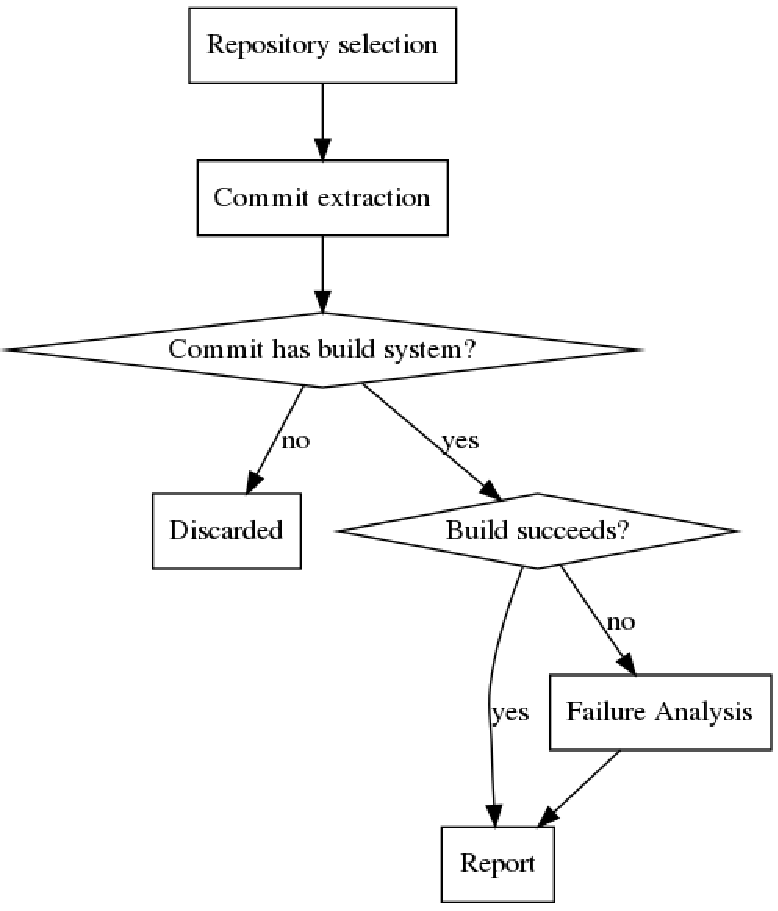
\includegraphics[height=0.8\textwidth]{pages/01-Buildability/images/Methodology.pdf}
\caption{Basic workflow for both studies.}
\label{fig:methodology}
\end{figure}


% Reduce separation between cells in next table
\renewcommand{\tabcolsep}{3pt}

\begin{table}[h]
\caption{Studies (main quantities)}
\label{table:statistics}
\begin{center}
\begin{tabular*}{\textwidth}{@{\extracolsep{\fill}}lrrrr}
\toprule
\textbf{Studies:}        & \textbf{Original} & \textbf{Original} & \textbf{Replic.} & \textbf{Reprod.} \\
                         & \textbf{Pristine} & \textbf{Reduced} \\
\midrule
Repositories             & 100               & 79                & 79               & 80      \\
Commits                  & 174,505           & 139,389           & 139,389          & 300,873 \\
Commits (build conf.)    & 132,484           & 101,811           & 101,811          & 281,487 \\
Commits (build success)  & 31,696            &  22,737           & 14,664           & 98,488  \\
\bottomrule
\end{tabular*}
%\caption*{
%  }
\end{center}

\begin{center}
\begin{tabular*}{\textwidth}{@{\extracolsep{\fill}}lrrrrrrr}
\toprule 
\textbf{Commits/project}  & \bf{min} & \bf{25\%} & \bf{50\%} & \bf{mean}  & \bf{75\%} & \bf{max}  & \bf{std} \\

\midrule
\bf{Replication}   &       25 &          234 &         726 &    1,764 &       1,898 &    14,818 & 2,694 \\
\bf{Reproduction}  &    1,132 &        1,974 &       2,980 &    3,760 &       4,847 &    10,000 & 2,404 \\


% Dejo esto aqui por si utilizamos estas cabeceras
% \bf{mean}  & 1,764.41  & 3,111.13 \\
% \bf{std}   & 2,694.93  & 1,825.44 \\
% \bf{min}   & 25       & 1,147    \\
% \bf{25\%}  & 234      & 1,791    \\
% \bf{50\%}  & 726      & 2,401    \\
% \bf{75\%}  & 1,898     & 3,693    \\
% \bf{max}   & 14,818    & 7,847    \\


\bottomrule
\end{tabular*}
\end{center}

\end{table}

% Restore original separation between cells
\renewcommand{\tabcolsep}{6pt}

There are some differences between the two studies, mainly on how we find repositories, which ones are our commits of interest in them, how we find those commits, and which build systems we consider (see details below). Table~\ref{table:statistics} shows some quantification (projects and commits) for the original study, with all its projects (\textit{Original Pristine}), for the reduced version of it, with the 79 repositories in which we could find all the commits (\textit{Original Reduced}), and for our replication (considering Maven builds only) and reproduction studies. The distribution of commits per project for the replication and reproduction studies is given as well.

% % Reduce separation between cells in next table
% \renewcommand{\tabcolsep}{3pt}

% \begin{table}[h]
% \caption{Basic statistics of projects}
% \label{table:statistics}
% \begin{center}
% \begin{tabular}{rrrrrrrr}
% \toprule 
% \bf{Study}    & \bf{min} & \bf{25\%} & \bf{50\%} & \bf{mean}  & \bf{75\%} & \bf{max}  & \bf{std} \\

% \midrule
% \bf{Replication}   &       25 &          234 &         726 &    1,764.41 &       1,898 &    14,818 & 2,694.93 \\
% \bf{Reproduction}  &    1,147 &        1,791 &       2,401 &    3,111.13 &       3,693 &     7,847 & 1,825.44 \\


% % Dejo esto aqui por si utilizamos estas cabeceras
% % \bf{mean}  & 1,764.41  & 3,111.13 \\
% % \bf{std}   & 2,694.93  & 1,825.44 \\
% % \bf{min}   & 25       & 1,147    \\
% % \bf{25\%}  & 234      & 1,791    \\
% % \bf{50\%}  & 726      & 2,401    \\
% % \bf{75\%}  & 1,898     & 3,693    \\
% % \bf{max}   & 14,818    & 7,847    \\


% \bottomrule
% \end{tabular}
% \end{center}
% \end{table}

% % Restore original separation between cells
% \renewcommand{\tabcolsep}{6pt}

\subsection{Replication Study}

For the replication study we followed the methodology of the original study as much as possible. Its authors considered 100 git repositories corresponding to Java FOSS projects from the ASF, all of them using a Maven-based build infrastructure. They retrieved in September 2014 all commits in their master branches, claiming to have analyzed a total of 219,395 commits. Then, they attempted to build all of them locally using Maven. The original paper comes with an accompanying reproduction package listing in detail which commits they considered for each repository. When reviewing that list, we found that the total number of commits referenced is 174,505. This is the reason why this is the number we include in the tables for the original study (see details in Section~\ref{sec:buildability:results-repli}).

\subsubsection{Subject Recovery}

Our first step was to retrieve the git repositories to analyze. We wanted to clone all the repositories, to be able of checking out each specific commit, and analyze its compilability. We were interested in doing a replication as close as possible, so we decided to use only the repositories for which we could find all the commits of the original study. This way, we ensured that results would be comparable, and not influenced by a potentially biased sample of missing commits.

We started by using the list of git repositories from the original study to clone and check all of them. We noticed that some were not available or did not have all the commits considered in the original study. From a total of 100 repositories in the list, 6 were no longer available. Before discarding them, we tried to find them both in the ASF git repositories, and in the GitHub repositories that the foundation maintains as replicas of the original ASF-hosted ones. In addition, of those that we could clone, 19 did not have all of the commits considered in the original study (8 had none of them, 11 had only some of them). This resulted in a total of 75 repositories with the complete set of commits considered in the original study. We followed this procedure during February 2020.

To improve the number of repositories with all commits from the original study,  we turned on to Software Heritage (SH), an initiative to collect, preserve and share all public source code in a universal software archive~\cite{di2017software,di2018software}. SH tries to archive all commits, even if they are later removed from the original repositories. Therefore, it was an option for finding the missing commits. Although its API is still evolving, during March 2020 we could use it to retrieve some of the repositories with missing commits, or which we could not find\footnote{In later conversations with representatives of Software Heritage, we learned that the part of the API for retrieving full repositories had been removed because it failed in some cases, which could explain our problems in retrieving some of the repositories.}.

We found all the 25 remaining repositories in SH, but as we retrieved them using their API, 5 of them were empty or corrupt, and of the other 20, only 4 contained all the commits of the original study.

Therefore, the dataset that we used for our replication study consisted of 79 repositories out of the 100 in the original study, amounting for 139,389 commits from the total of 174,505 commits (79,9\%). Even when this is only a fraction of the commits, we consider that the sample is large enough to conduct the rest of the study, as follows.

\subsubsection{Building}

Once we cloned all git repositories, we proceeded to replicate the experiment. For that, we checked out, one by one, all source code snapshots, each one corresponding to one commit, and tried to build them. In the original study they used some Java program to run the Maven tool, via its Java API, to build the code. However, we could not find the code in their reproduction package. Because of this, but also because we wanted to produce a tooling-independent replication, we developed a Python script that uses Maven through its command-line interface. The design of the script allowed to include other build systems, to be used in the reproduction study.

\begin{figure}[t]
\centering    
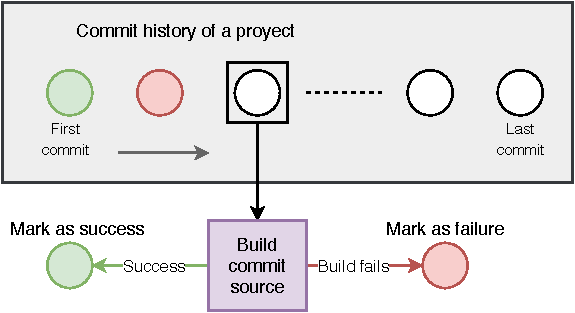
\includegraphics[width=\textwidth]{pages/01-Buildability/images/AnalysisProcess.pdf}
\caption{Process for checking compilability status of commits in a repository. ``Build commit source'' includes checking out the commit, checking for Maven configuration files, and if found, running Maven to try to build the code.}
\label{fig:commitHist}
\end{figure}

For each commit of interest in each repository, the script runs the following procedure (see also Figure~\ref{fig:commitHist}):
\begin{enumerate}
\item Check out the intended commit, obtaining the snapshot of the source code to be built.
\item Find the configuration for Maven (usually a \verb|pom.xml| file). If it is found, the build command for Maven is executed (\textit{mvn clean compile -X}) in a Docker container spawned for this specific analysis.
\item Collect the status code and the log produced by the execution in a log file (the verbose option of the command is used to obtain the most detailed log). If a configuration for Maven was not found, it is also noted in the log file.
\end{enumerate}

A further analysis of the log file allowed us to identify if the snapshot had configuration files for Maven, if the build was successful or not, and if not, the likely reason for the failure.

% jgb: SIZE. Remove next para if needed.
It is important to ensure the build environment is fully clean from results of previous builds, such as dependency modules or intermediate files that could influence the current one. To enforce this cleanup, besides the build command cleaning up local folders, the execution is encapsulated in a Docker container containing Maven and Java 8.

When checking for the presence of a Maven configuration file, we found an important replication issue: in all projects but three, those files were in exactly the same commits than the original study. But in those three, we found many more commits with Maven configuration (in the order of 6,000). We carefully inspected the checkout for a large sample of those commits, and our heuristics seem to work well. Unfortunately, this has some impact on the results of the replication, especially since a fraction of them are actually compilable. For having a more usable comparison with the results of the original study, we decided to analyze those commits separately (see details in Section~\ref{sec:buildability:results-repli}), so that the results on how compilability ``ages'' are not influenced because of them. That is the reason why the number of ``Commits (build conf.)'' in Table~\ref{table:statistics} is exactly the same (101,811) in both the original study (reduced) and our study (for the 79 considered repositories).

When searching for build files (pom.xml), we discovered that we were able to detect 4.72\% more commits with build files than the authors of the original study.
Detecting the presence of these build files is a relatively simple task, as they are easy to identify if they exist.
Nonetheless, to check if this inconsistency was due to an error in our scripts, we randomly selected a dozen commits where we found build files but the original study did not, and performed a manual inspection.
We found that our approach is the correct one.
So, probably the discrepancy is caused by some bug in the scripts of the original paper. As these scripts are not publicly available, we cannot confirm this possibility.

To explore the compilability of all of the snapshots, we used two Ubuntu 18.04 machines, one of them with 16 cores and 8 GB of RAM and the other one with 8 cores and 16 GB of RAM. The software we built was capable of balancing the load between both servers to minimize execution time, building several snapshots in parallel. Once the repositories to analyze were ready, the building of all snapshots took about four weeks of wall time to run.

\subsubsection{Obtaining Results}

The results of the study are obtained from analyzing the log file. From it, we can know if a Maven configuration was found for a commit, or if the build was successful. For the analysis on the causes of build failures, we analyze the exception produced by Maven from the log for the failed builds. The exceptions that can be produced during the construction of the Maven project are well defined and limited\footnote{https://cwiki.apache.org/confluence/display/MAVEN/Errors+and+Solutions}. For the reporting, we use the classification and mapping of exceptions in the original study, which defined four categories of errors: \textit{Resolution} (related resolution of artifacts, such as downloading of dependencies), \textit{Parsing} (such as malformed build configuration), \textit{Compilation} (during the compilation phase) and \textit{Other}. Note that the first three correspond to the first three steps in the building process described in~\cite{Sulir:2016:QSJ:3001878.3001882}, presented in Section~\ref{sec:buildability:related}.

For comparing our results with the original study, we also classified every commit according to how it behaved when building it in both studies:
%\begin{itemize}
\begin{inparaenum}[\bf(1)]
  \item \textbf{stable build}, the snapshot was built in both studies;
  \item \textbf{new error}, the snapshot was built in the original study, but not in ours;
  \item \textbf{same error}, the build failed in both studies for the same reason;
  \item \textbf{different error}, the build failed in both studies but for a different reason; and,
  \item \textbf{new build}, the build failed in the original study but not in ours.
\end{inparaenum}
%\end{itemize}

We tried to reproduce the methods of the original study as much as possible, using the same classification to enable a comparison as is mandatory in a replication study.
However, we did not do it manually but automated the procedure.
We took therefore advantage of the description of the Java exceptions used in their classification by the original authors in their reproduction package\footnote{http://www.cs.wm.edu/semeru/data/breaking-changes/}.
As each exception is mapped to exactly a single category, our tool took this mapping and applied it automatically, avoiding the necessity for a manual classification.
We think this highlights one of the main reasons for replication studies: to be able to detect and fix limitations in previous works.
Our tool and data sources are publicly available in our reproduction package.


\subsection{Reproduction study}

\subsubsection{Subject selection and recovery}

For our reproduction study, we generated a new dataset of repositories to analyze. Inspired by~\cite{Sulir:2016:QSJ:3001878.3001882}, we obtained a long list of repositories via the GitHub API, meeting the following criteria:

\begin{itemize}
\item \textit{Java as the programming language}. We wanted to check Java building technologies, staying in the same domain of the original study.
\item \textit{At least 500 stars and 300 forks}. We wanted some indicator of relevance.
\item \textit{At least five years of development}. We wanted to have a long enough commit history, so that the analysis was more complete.
\item \textit{Active in January 2020} (at least one commit). We wanted projects with recent activity, to include current practices.
\item \textit{Use a build system}. We wanted to check compilability, so we checked that they were using Maven, Gradle or Ant (the three most popular build systems for Java) in the last commit.
\item \textit{Between 1,000 and 10,000 commits}. We wanted to avoid projects too small, which would have few snapshots to analyze, but also very large ones, which would consume too many resources for the analysis.
\item \textit{No Android projects}. Because of a practical limitation: building projects for Android is in general more complex, and requires specific procedures.
\end{itemize}

From the long list meeting all these conditions, we randomly selected repositories for our reproduction study and proceeded to their analysis.
For each repository, we considered all commits in the master branch as the commits of interest for the study. 
A total of 80 projects have been selected for this reproduction study.
The total number of commits was 300,873.
When comparing the resulting list with the list of projects from the original analysis, in addition to variety (since the previous analysis was focused only in ASF projects), the main difference is that we focused in non-small projects with certain relevance.

\subsubsection{Building}

The process we followed to explore the buildability of snapshots for the repositories in our list was very similar to the one described above for the replication study. The differences were as follows:

\begin{itemize}
\item After checking out a commit, three systems are considered when searching for build configuration (see ``Build File'' in Table~\ref{table:buildSystems}). In the replication study only Maven was considered.
\item When building the snapshot with more than one build system, we tried the build systems in order: first Maven or Gradle, and if it failed, then Ant. We did not find snapshots with both Maven and Gradle. Having Ant and one of Maven or Gradle is usually due to the project transitioning from the former to the latter, thus still having the old Ant configuration and a new configuration for Maven or Gradle. Our order for testing systems considers that if the Maven or Gradle configuration worked, the project had likely already transitioned to them, if it did not, the project was still with Ant.
\item For each build configuration, we executed the build command defined by the build configuration (see ``Command'' in Table~\ref{table:buildSystems}).
\end{itemize}

\begin{table}[h]
  \caption{Build systems considered in the reproduction study}
  \label{table:buildSystems}
  \centering
  \begin{tabular*}{\textwidth}{@{\extracolsep{\fill}}lll}
    \toprule
    \bf{Build System} & \bf{Command} & \bf{Build File}\\
    \midrule
    Maven & mvn clean compile -X & pom.xml\\
    Gradle & ./gradlew build -x test & build.gradle \\
    Ant & ant compile  & build.xml \\
    \midrule
  \end{tabular*}
\end{table}
 
For this reproduction study, the Docker container we used included Java 8, Ant and Maven, while Gradle was run standalone (since it works self-contained). 
%Once the repositories to analyze were ready, 
The building of all snapshots took about two weeks of wall time, in the same environment we used for the replication study.


\subsubsection{Obtaining results}

As we did for the replication study, the results of the reproduction study are obtained by analyzing the logs of the attempts to build each considered commit from our list of repositories. The analysis is the same that we described already, with the difference that in the reproduction study we considered not only if the snapshot could be built or not, but also which build system was used. We also had to extend the mapping of exceptions in error logs to one of the four categories of errors in the original study (\textit{Dependency}, \textit{Parsing}, \textit{Compiling} or \textit{Other}). 
The new error mapping will be shown in the following sections, as well as being available in the reproduction package.


\section{Replication Study: Results}
\label{sec:buildability:results-repli}
% REPLICATION RESULTS

\subsection{Data for replication}

The original paper comes with a reproduction package, which we have found tremendously useful. It includes the complete list of commit hashes for all the analyzed repositories, and counts per repository of the main results. This allowed us to compute counts for our reduced set of 79 repositories. This way, we could do a fair comparison between the replication and the original results.

After computing our results for the 79 repositories in the original study, we found a discrepancy in the total number of commits. According to the original paper, 219,395 commits were analyzed. But computing from the list of commit hashes, we counted 174,505. To be consistent with other data in our study, which was extracted from that reproduction package, we used the second number in our tables. This fact does not impact the results, since we focus on the analysis of the reduced set of 79 repositories.

The scripts used for the original study are not available in its reproduction package. This is not a problem in itself, since we created our own software. But we could not determine the reason for some discrepancies, e.g., on the number of snapshots with build configuration (see details below). Maybe the heuristics coded into the original software took into account something that we missed, or maybe it didn't detect that configuration information in some cases.

Detailed logs of the execution are also not available in the reproduction package of the original study, making it difficult to explain some differences found in the compilability of a large number of commits in three repositories (see details below): we do not know if there was some error in the execution of the original study, or if we are missing something in our own.

\vspace{0.3cm}
\fbox{\begin{minipage}{0.9\textwidth}
\textbf{\textbf{RQ\textsubscript{1.1d}}: ``Is the data in the reproduction package of the original study enough for a replication?''} There is enough data for comparing results, even at the repository level. However, there is not enough data to exactly reproduce the original study: a copy of the git repositories, as they were when the analysis was performed, is missing; some relevant software is also missing (such as the one to detect the Maven configuration in a snapshot); and the logs of their execution for all snapshots is also missing, which makes it difficult to understand the reasons of some discrepancies when replicating the study.
\end{minipage}}

\subsection{Compilability}

To answer RQ\textsubscript{1.1a} and RQ\textsubscript{1.1c} in detail, we follow the same process as the original study, classifying repositories in three categories according to their number of commits: short history (number of commits in the first quartile, Q1), medium history (Q2 and Q3) and long history (Q4). Repositories classified as short (20) have less than 203 commits, medium (39 repositories) have between 203 and 1,148 commits, and long repositories (20) have more than 1,148 commits. Then, we analyze the compilability of those snapshots for which we found configuration for Maven, assuming the rest could not be built because developers were not using automatic tools for building.

Tables~\ref{table:replication-compilability} and \ref{table:replication-compilability-2} shows the results for compilability in the original study, and of our replication study. For the original study we computed, thanks to the details in its reproduction package, results for the reduced list of 79 repositories that we have analyzed. However, the results for the pristine study (with all its 100 repositories) are very similar to those of the reduced one. For example, the average compilability of the reduced study is 37.19, while for the pristine study it is 38.13, according to the original paper. For completeness, we run Wilcoxon's test on the compilability results of all projects of the previous and our replication studies, obtaining a p-value of 1.9077e-6. This confirms statistical significant differences between both cases.

% TABLE 1
\begin{table*}[h]
\caption{Compilable snapshots - Distribution (top: Reduced Original Study, bottom: Replication Study).}
%\label{table:originalResultsCompilability}
\label{table:replication-compilability}
\begin{center}
\resizebox{\textwidth}{!}{%
  \begin{tabular}{llllllll}
  \toprule
    \bf{Projects} & \multicolumn{7}{l}{Fraction built (in \%)} \\
                  & \multicolumn{7}{l}{} \\
                  & \bf{Min} & \bf{1st Qu.} & \bf{Median} & \bf{Mean} & \bf{3rd Qu.} & \bf{Max} & \bf{SD} \\  
  \midrule
  Short history  & 0.00     & 23.67        & 48.64       & 49.85      & 82.73       &  97.01   & 35.08 \\ 
  Medium history & 0.00     &  4.99        & 36.24       & 38.43      & 68.42       & 100.00   & 34.03 \\
  Long history   & 0.00     &  0.00        & 16.48       & 22.14      & 25.67       & 100.00   & 29.33 \\
  \midrule
  All            & 0.00     & 2.91         & 28.64       & \bf{37.19} & 66.00       & 100.00   & 34.25 \\ 
  \bottomrule
  \end{tabular}
}
\end{center}

\begin{center}
\resizebox{\textwidth}{!}{%
  \begin{tabular}{llllllll}
    \toprule
    \bf{Projects} & \multicolumn{7}{l}{Fraction built (in \%)} \\
                  & \multicolumn{7}{l}{} \\
                  & \bf{Min} & \bf{1st Qu.} & \bf{Median} & \bf{Mean} & \bf{3rd Qu.} & \bf{Max} & \bf{SD} \\  
  \midrule
  Short history  & 0.00     & 0.55         & 31.49       & 40.62      & 82.72        & 99.01     & 39.97 \\ 
  Medium history & 0.00     & 0.00         & 1.70        & 20.99      & 38.24        & 95.23     & 29.52 \\ 
  Long history   & 0.00     & 0.00         & 9.44        & 17.56      & 19.17        & 100.00    & 28.31 \\ 
  \midrule
  All            & 0.00     & 0.00         & 8.74        & \bf{25.1}  & 41.64        & 100.00    & 33.07 \\ 
  \bottomrule
  \end{tabular}
}
\end{center}
\end{table*}


%% TABLE 2
\begin{table*}[h]
  \caption{Compilable snapshots - Totals (top: Reduced Original Study, bottom: Replication Study).}
  %\label{table:originalResultsCompilability}
  \label{table:replication-compilability-2}
  \begin{center}
  
  \begin{tabular*}{\textwidth}{l|llllllll|lll}
  \toprule
    \bf{Projects} & \multicolumn{3}{c}{Total commits} \\
                  & \multicolumn{1}{c}{\bf{with build conf.}} & \multicolumn{1}{c}{\bf{Build success}} & \multicolumn{1}{c}{\bf{Fraction built}} \\
  \midrule
  Short history  &   2,311 &  1,129 & 48.85\% \\ 
  Medium history &  26,903 &  9,602 & 35.69\% \\
  Long history   &  72,597 & 12,006 & 16.54\% \\
  \midrule
  All            & 101,811 & 22,737 & 22.33\% \\ 
  \bottomrule

  \midrule
  Short history  &   2,311 &    876 & 37.91\%\\ 
  Medium history &  26,903 &  6,049 & 22.48\%\\ 
  Long history   &  72,597 &  7,739 & 10.66\%\\ 
  \midrule
  All            & 101,811 & 14,664 & 14.40\%\\ 
  \bottomrule
  \end{tabular*}
  \end{center}
\end{table*}



\vspace{0.2cm}
\fbox{\begin{minipage}{0.9\textwidth}
\textbf{ \textbf{RQ\textsubscript{1.1a}}: ``How many snapshots from the change history are compilable?''} 8.74\% or less of the commits were compilable for half of the analyzed projects. The result for the original study was 28.64\%.
Thus, results are very different, likely affected by the time passed (as we will discuss when answering RQ\textsubscript{1.1c}).
\end{minipage}}

\fbox{\begin{minipage}{0.9\textwidth}
\textbf{\textbf{RQ\textsubscript{1.1c}}: ``Has compilability degraded since the original study?''}
A much smaller fraction of the commits with build configuration can be built (22.33\% in the original study versus 14.66\% in our replication). When analyzing repositories by size, medium projects are more affected by this decrease in compilability, with half of them having a compilability of 1.70\% or less, while in the original study that number was 36.24\%. Short projects are also affected, and the less affected are long projects, but still they move from a median of 16.48\% to 9.44\% in our replication.
\end{minipage}}
\vspace{0.2cm}

We found significant differences in three repositories when checking for the existence of Maven configuration files (for all the others, results are exactly the same). In those three repositories we found 6,583 extra commits with a Maven configuration. When trying to build them, we could build 442 extra snapshots, which would increase the number of compilable snapshots to 15,106 (from a total of 108,394), or 13.93\% compilability, slightly less than 14,40\, as shown in Table~\ref{table:replication-compilability-2}.

We also checked all snapshots for configuration files of Ant and Gradle (we only found for Ant), finding 2,586 additional snapshots that could be built, leading to a total of 17,692 commits built. However, these results are not comparable with the original study, since they did not consider Ant.

Table~\ref{table:replication-buidability-summary} summarizes the results of all replications, with the different cases.
It should be noted that Table~\ref{table:replication-compilability} extends the information of the results reported in the ``Replication'' row of Table~\ref{table:replication-buidability-summary}, as it is the most comparable scenario between the original and the replication study.

\begin{table*}[h]
\caption{Original and replication studies (Summary of results). Replication\textsubscript{a}: use same build configs, Replication\textsubscript{b}: use all detected Maven config files, Replication\textsubscript{c}: use all detected Maven and Ant config files}
\label{table:replication-buidability-summary}
\resizebox{\textwidth}{!}{%
  \begin{tabular}{lrrrrrr}
  \toprule
  & Repos.                        & All     & Commits           & Commits & Built & Built \\
  &                              & Commits & w/build conf    & built   & total          & mean of\\
  &                              &         &                   &         &                & projects \\
  \midrule 
  Pristine Original               & 100     & 174,505 & 132,484 & 31,696  & 23.92\%        & 37.74\% \\
  Reduced Original                &  79     & 139,389 & 101,811 & 22,737  & 22.33\%        & 37.19\% \\
  Replication\textsubscript{a}    &  79     & 139,389 & 101,811 & 14,664  & 14.40\%        & 25.09\% \\
  Replication\textsubscript{b}    &  79     & 139,389 & 108,394 & 15,106  & 13.93\%        & 25.42\% \\
  Replication\textsubscript{c}    &  79     & 139,389 & 117,124 & 17,692  & 15.10\%        & 24.85\% \\  
  \bottomrule
  \end{tabular}
}
\end{table*}


\subsection{Failure analysis}

To answer RQ\textsubscript{1.1b}, and provide some insight on the reasons for the answer to RQ\textsubscript{1.1c}, we analyzed build failures following the categorization of the original study. Table~\ref{table:allCauses} reports the classification results for the previous study and for our replication, in both cases for the 79 repositories of the reduced study.

\begin{table}[h]
\caption{Causes of failed builds.}
\label{table:allCauses}
\begin{center}
\begin{tabular*}{\textwidth}{@{\extracolsep{\fill}}rrrrr}
\toprule
\multicolumn{1}{l}{}	    & \multicolumn{2}{c}{\bf{Original study}}    & \multicolumn{2}{c}{\bf{Replication study}}  \\
\bf{Categories}                 & \multicolumn{1}{r}{\#} & \multicolumn{1}{r}{\%} & \multicolumn{1}{r}{\#} & \multicolumn{1}{r}{\%}  \\
\midrule
Resolution  & 47,832 &  60.49 & 55,299 & 63.45  \\
Parsing     &  9,595 &  12.13 & 10,350 & 11.88  \\
Compilation &  2,807 &   3.55 &  2,544 &  2.92  \\
Other       & 18,839 &  23.83 & 18,954 & 21.75  \\
\midrule
All errors & 79,073 & 100.00 & 87,147 & 100.00 \\
\bottomrule
\end{tabular*}
\end{center}
\end{table}

Table~\ref{table:causesDetailed} shows the changes we observed when building snapshots with respect to the original study, according to the classification provided in Section~\ref{sec:buildability:metodology}. We could build 14,480 (63.68\%) of the successful builds in the original study (\textit{stable builds}). We could also build some snapshots that could not be built in the original study. In general, these correspond to external artifacts that were not available when they run their experiments, but were available when we run ours. These \emph{new build} snapshots amount to 184 (0.13\%).

% jgb: Keeping this old table, with only errors, in case we need to
% revert to it because of size limits (and write the data about new and
% stable builds somewhere else
%
% \begin{table}[]
% \caption{Changes in causes of failed builds}
% \label{table:causesDetailed}
% \begin{tabular}{rrrrrrr}
% 	\toprule
% \multicolumn{1}{l}{\bf{Categories}} & \multicolumn{2}{c}{\bf{Same error}} & \multicolumn{2}{c}{\bf{Different error}} & \multicolumn{2}{c}{\bf{New error}} \\
% \bf{(Replication)} & \multicolumn{1}{c}{\#} & \multicolumn{1}{c}{\%} & \multicolumn{1}{c}{\#} & \multicolumn{1}{c}{\%} & \multicolumn{1}{c}{\#} & \multicolumn{1}{c}{\%} \\
% \midrule
% Resolution & 42,826  & 49.14  & 4,704 & 5.39  & 4,868  & 5.59                    \\
% Parsing                & 9,485                   & 10.88                   & 694                     & 0.79                    & 171                     & 0.20                    \\
% Compilation            & 2,544                   &  2.91                   & 0                       & 0.00                    & 0                       & 0.00                    \\
% Other                  & 12,443                  & 14.27                   & 6,194                   & 7.10                    & 3,218                   & 3.69                    \\
% \midrule
% All errors & 67,298 & 77.22 & 11,592 & 13.30 & 8,257 & 9.48 \\                 
% \bottomrule
% \end{tabular}
% \end{table}

\begin{table}[]
\caption{Changes in builds (original to replication).}
\label{table:causesDetailed}
\centering
\resizebox{\textwidth}{!} & \multicolumn{1}{c}{\#} & \multicolumn{1}{c}{\%} & \multicolumn{1}{c}{\#} & \multicolumn{1}{c|}{\%} & \# & \# \\
  \midrule
  Resolution             & 42,826                  & 49.14                   & 7,605                   & 5.39                    & 4,868                   & 5.59                    \\
  Parsing                & 9,485                   & 10.88                   & 694                     & 0.79                    & 171                     & 0.20                    \\
  Compilation            & 2,544                   &  2.91                   & 0                       & 0.00                    & 0                       & 0.00                    \\
  Other                  & 12,443                  & 14.27                   & 3,293                   & 7.10                    & 3,218                   & 3.69                    \\
  \midrule
  All  & 67,298 & 77.22 & 11,592 & 13.30 & 8,257 & 9.48 & 14,480 & 184 \\ 
  \bottomrule
  \end{tabular}
}
\end{table}

For 67,298 of the snapshots that failed to build, we reported the same exception as in the previous experiment (\textit{same error}). Therefore, adding these to \textit{stable build}, 81.778 (80.66\% of the snapshots with build configuration) behaved exactly as in the original study. On the other hand, for 13.30\% of the snapshots that failed for us, we found a different error than in the original study (\textit{different error}), while 9.48\% of the snapshots that failed for us did not fail in the original study (\textit{new error}).

Both in \textit{different error} and in \textit{new error}, one of the main causes for failed builds is \textit{Resolution}, and specifically, the resolution of external artifacts needed for the build. We can affirm that one of the main reasons for the degradation in compilability with time is the impossibility of recovering more and more of the dependencies of these projects as time passes. On the other hand, \textit{Compilation} errors only appear in \textit{same error}, since they only depend on using the same compiler (so if they failed in the replication, they should have failed in the original study). Comparing the number of \textit{Compilation} errors in the replication and in the original study, it decreased from 2,807 to 2,544. Some inspection raised the cause: new exceptions mask previous building errors.

% jgb: SIZE We could remove the next para if needed
We studied in some detail the \textit{Resolution} category. One of the most recurrent cause was experiencing timeouts when accessing some external artifact, usually a dependency (5.12\% of total errors). This type of error appears only as \textit{different error} or \textit{new error}. Given that no long network failures were observed during the execution of our study, this is due to access to artifacts that are no longer available, which is consistent with the previous comment on dependencies.

\vspace{0.2cm}
\fbox{\begin{minipage}{0.9\textwidth}
\textbf{\textbf{RQ\textsubscript{1.1b}}: ``What types of errors prevent snapshots from being built?''}
The proportion of the different kinds of errors is similar to the original study. Most of the errors (63.45\%) are caused by resolution of dependencies and other external artifacts (60.49\% for the original study), these being the errors that contributed the most to the degradation of compilability. Parsing errors convey 11.88\% of the failures we detected, close to the 12.13\% reported in the original study. The same can be said for Compilation errors (2.92\% in our replication \emph{vs.} 3.55\% in the original study). About 80\% of the snapshots behaved exactly like in the previous study (they built, or they failed with the same error).
\end{minipage}}


\section{Reproduction Study: Results}
\label{sec:buildability:results-repro}
% REPRODUCTION RESULTS

\subsection{Compilability}

To answer RQ\textsubscript{1.2a}, we repeated the same analysis of the replication study, but now for the 80 projects of our reproduction study. Of them, 20 projects were classified as having a short history (Q1, less than 1,974 commits), 40 as medium history (Q2 and Q3), and 20 as long history (Q4, more than 4,847 commits). Compilability results are shown in Table~\ref{table:results-reproduction}.

\begin{table*}[h]
\caption{Reproduction study - Compilability results}
%\label{table:ourResultsCompilabilityReproduction}
\label{table:results-reproduction}


% TABLE 1
\begin{center}
\resizebox{\textwidth}{!}{%
  \begin{tabular}{@{\extracolsep{\fill}}l|lllllll|lll}
  \toprule
    \bf{Projects} & \multicolumn{7}{c}{Fraction built (in \%)} & \multicolumn{3}{c}{Total commits}\\
    \bf{by history} & \multicolumn{7}{c}{} & \bf{with} & \bf{Build} & \bf{Fraction} \\
                  & \bf{Min} & \bf{1st Qu.} & \bf{Median} & \bf{Mean} & \bf{3rd Qu.} & \bf{Max} & \bf{SD} & \bf{build conf.} & \bf{success} & \bf{built}\\   
  \midrule
  Short          & 0.00     & 37.43        & 55.42       & 58.21          & 82.27 &  99.38 & 28.12  & 28,312 & 15,948 & 56.32\%\\
  Medium         & 0.00     & 10.56        & 34.94       & 40.35          & 68.60 & 100.00 & 33.34 & 114,716 & 44,688 & 38.96\%\\
  Long           & 0.00     & 4.27        & 12.80       & 27.76          & 48.04 &  93.52 & 31.76 & 138,459 & 37,852 & 27.33\%\\
  \midrule
  All            & 0.00     & 10.56        & 36.25       & \textbf{41.66} & 70.62 & 100.00 & 33.18 & 281,487	 & 98,488	 & 34.98\%\\
  \bottomrule
  \end{tabular}
}
\end{center}

% % TABLE 2
% \begin{center}
% \begin{tabular*}{\textwidth}{@{\extracolsep{\fill}}l|lll}
% \toprule
%   \bf{Projects} & \multicolumn{3}{c}{Total commits} \\
%                 & \multicolumn{1}{c}{\bf{with}} & \multicolumn{1}{c}{\bf{Build}} & \multicolumn{1}{c}{\bf{Fraction}} \\
%                 & \bf{build conf.} & \bf{success} & \multicolumn{1}{c}{\bf{built}}\\    
% \midrule
% Short history  & 28,312 & 15,948 & 56.32\%\\
% Medium history & 114,716 & 44,688 & 38.96\%\\
% Long history   & 138,459 & 37,852 & 27.33\%\\
% \midrule
% All            & 281,487	 & 98,488	 & 34.98\%\\
% \bottomrule
% \end{tabular*}
% \end{center}

\end{table*}

% TABLE 3

\begin{table*}[h]
  \caption{Reproduction study - Compilability by build system.}
  \label{table:results-reproduction-build-systems}

\begin{center}
  \begin{tabular*}{\textwidth}{@{\extracolsep{\fill}}l|rrr}
  \toprule
  \bf{BuildSystem} & \multicolumn{3}{c}{Compilability}                                  \\
  \bf{}	& \bf{\#Commits} & \bf{\#Build success} & \bf{Fraction built} \\
  \midrule
  Maven           &        191,063  &                     80,310 &            42.03\%  \\
  Ant             &         25,735  &                      4,441 &            17.26\%  \\
  Gradle          &         64,095  &                     13,737 &            21.43\%  \\
  \midrule
  All             &        280,893  &                     98,488 &            35.06\%  \\
  \bottomrule
  \end{tabular*}
\end{center}

\end{table*}

% TABLE 4

\begin{table*}[h]

  \caption{Reproduction study - Errors by build system.}
  \label{table:results-reproduction-build-systems-errors}

\begin{center}
\resizebox{\textwidth}{!} & \bf{\#} & \bf{\%}  & \bf{\#} & \bf{\%}  & \bf{\#} & \bf{\%} \\
  \midrule
  Maven           &          75,806 &             68.45\%  &        1,967 &            1.78\% &                0 &                0.00\% &     32,980 &        29.78\% \\
  Ant             &           4,485 &             21.06\%  &            0 &            0.00\% &            1,077 &                5.06\% &     15,732 &        73.88\% \\
  Gradle          &          22,260 &             44.20\%  &            0 &            0.00\% &            2,373 &                4.71\% &     25,725 &        51.08\% \\
  \midrule
  All             &         102,551 &             56.22\%  &        1,967 &            1.08\% &            3,450&                1.89\% &     74,437 &        40.81\% \\
  \bottomrule
  \end{tabular}
}
\end{center}

\end{table*}

For all categories, and for all the projects together, median and mean are close, meaning the distribution is not very skewed: to some extent we were successful in avoiding bias when selecting projects to analyze.  
The standard deviation shows a large spread in the values (compatible with the values observed for the different quartiles). 
The fraction of snapshots that could not be built in all categories is higher than (or very close to) 50\%, which shows that automatic compilability of past snapshots can certainly not be given for granted. 
Projects with a long history have in general less compilability, and compilability increases as we move to projects with a medium and short history.

It should be noted that in the original study, we found a great diversity in the size of the projects according to their number of commits (from projects with 25 commits to 14k).
The problem with smaller projects ($<$203 commits) is that in many cases they have not had a natural development (the initial commit imports code from another source, as can be seen for example in following commit\footnote{https://github.com/apache/maven-app-engine/commit/b77ad9e82d7cc94}).
This means that part of the project's development history is lost, which is a limitation of the original study.
In the selection criteria for the repository mining we have taken this limitation into account, setting a lower limit of 1000 commits.
Because of this difference between experiments, the separation between small, medium and large projects is different and the groups cannot be compared between experiments. 
Nonetheless, for the sake of completeness, we offer a comparison using the same quartiles to classify the projects into the three categories in a table that can be found in the replication package.

\vspace{0.2cm}
\fbox{\begin{minipage}{0.9\textwidth}
\textbf{\textbf{RQ\textsubscript{1.2a}}: ``How many snapshots from the change history are compilable?''}
Less than half of the snapshots with build configuration could be built. Compilability decreased with the size of the commit history of projects. For all history size categories, and all projects together, mean and median compilability was less than 51\%, although variability is high (standard deviation is over 28\% in all cases).
\end{minipage}}

\subsection{Failure analysis}

To answer RQ\textsubscript{1.2b}, we analyzed build failures, as shown in Table~\ref{table:results-reproduction-build-systems-errors}. Most of the errors are of type \textit{Resolution}, due to missing dependencies and other external artifacts. \textit{Parsing} and \textit{Compilation} errors are almost negligible.

% \begin{table}[h]
% 	\caption{Causes of failed builds (Reproduction Study)}
% 	\label{table:resultsGithub}
% 	\begin{center}
% 	\begin{tabular}{rrr}
% 		\toprule
% 		\bf{Action}  & \bf{\#} & \bf{\%} \\
% 		\midrule
% 		Resolution      &  32,671   &  56.32 \\
% 		Parsing         &     970   &   1.67 \\
% 		Compilation     &   1,248	&   2.15 \\
% 		Other           &  23,125   &  39.86 \\
% 		\midrule
% 		All            &   58,014   & 100.00 \\
% 		\bottomrule
% 	\end{tabular}
% 	\end{center}
% \end{table}

The fact that most errors are due to missing external objects is a good indicator of further decline of compilability in the future: as time passes, more and more artifacts will disappear, which will lead to more and more commits not building. The low numbers for \textit{Parsing} and \textit{Compilation} errors are interesting: they could be indicating that the use of automatic tools to check the compilability of snapshots (and therefore, the consistency of building configuration, and the correctness of compilation) before merging the corresponding commits.

\vspace{0.2cm}
\fbox{\begin{minipage}{0.9\textwidth}
\textbf{\textbf{RQ\textsubscript{1.2b}}: ``What types of errors prevent snapshots from being built?''}
Most of the errors observed (56\%) are due to missing dependencies and other external artifacts. The impact of these errors in the overall compilability is thus very important: almost one third (36.43\%) of all snapshots with building configuration could not be built because of them. However, parsing and compilation errors are few, meaning that most snapshots were carefully checked for these errors before committing.    
\end{minipage}}


\subsection{Building system}

To answer RQ\textsubscript{1.2c}, we performed an analysis by build system. When we were detecting build configuration files, we observed some projects starting to build with Ant, then switching to Maven or Gradle, and some others using Maven and Gradle for their entire history. From the total number of commits with build configuration, 68.02\% are for Maven, 22.82\% for Gradle, and 9.16\% for Ant. The results of the analysis by build system are shown in Table~\ref{table:results-reproduction-build-systems}.

The first interesting result is that compilability for snapshots with Maven is much higher (42.03\%) than for Ant or Gradle (17-22\%). With respect to specific kinds of errors, Maven is dominated by \textit{Resolution}, as Gradle and Ant is dominated by \textit{Other}. However, the sample of snapshots with Ant and Gradle is relatively small, which means our results for them are less reliable.

The detailed classification of errors for all building systems can be found in the Table~\ref{table:other-errors} (The table is limited to the 20 most frequent errors, the full table can be found in the reproduction package). 
From this classification, it is worth mentioning:
\begin{itemize}
 \item From the 15,732 \textit{other errors} for Ant, 8,615 are failures because they do not have the ``compile'' task defined (which is a standard in the development of projects with Ant), and about 4,610 because a specific binary or config file is expected in the path, instead of being included as a dependency.
 \item From the 25,725 \textit{other errors} for Gradle, 5,215 of them fail because of a test that cannot be automatically ignored. A common error (4,726) is that some tasks, defined as scripts in the configuration file by the developer, fail to build the project. Other less common errors are the absence of a secret key (which is not usually stored in a public repository), an error in the generation of documentation or the lack of permissions for certain system folders. These errors, although a priori generic, are usually concentrated in a single project and are not significant.
\end{itemize} 

Although all of these snapshots could not be built automatically, they could be built with minimal human intervention, or with a slightly improved set-up of the build configuration for the projects affected. Given the relatively small sample of snapshots for these two systems (Ant and Gradle, compared to Maven), considering these snapshots as errors or not would change dramatically the figures for the \textit{other errors} category for both of them. In the reporting of results, we have decided to consider those cases as errors, which is a cause for the lower compilability reported for Ant and Gradle.

\newpage

\begin{table}[]
  \caption{Classification of errors for all build systems}
  \label{table:other-errors}
\resizebox{\textwidth}{!} \\ \hline
  Maven                & ArtifactResolutionException        & Resolution      & 74,950          & 41.09       \\ \hline
  Maven                & MojoFailureException               & Other           & 12,426          & 6.81        \\ \hline
  Maven                & MojoExecutionException             & Other           & 11,562          & 6.34        \\ \hline
  Ant                  & Target "compile" does not exist    & Other           & 8,615           & 4.72        \\ \hline
  Gradle               & IOException: Server returned ...   & Resolution      & 8,057           & 4.42        \\ \hline
  Gradle               & Could not resolve                  & Resolution      & 7,057           & 3.87        \\ \hline
  Gradle               & Could not resolve all dependencies & Resolution      & 6,899           & 3.78        \\ \hline
  Maven                & ConnectException                   & Other           & 5,524           & 3.03        \\ \hline
  Gradle               & Task 'test' not found              & Other           & 5,215           & 2.86        \\ \hline
  Gradle               & Execution failed for task          & Other           & 4,726           & 2.59        \\ \hline
  Gradle               & Cannot run program                 & Other           & 4,540           & 2.49        \\ \hline
  Ant                  & UnknownHostException               & Resolution      & 3,918           & 2.15        \\ \hline
  Gradle               & Other Gradle error                 & Other           & 3,849           & 2.11        \\ \hline
  Ant                  & Unable to find property file       & Other           & 3,693           & 2.02        \\ \hline
  Gradle               & Permission denied                  & Other           & 2,295           & 1.26        \\ \hline
  Gradle               & Compilation failed                 & Compilation     & 2,288           & 1.25        \\ \hline
  Maven                & PluginDescriptorParsingException   & Parsing         & 1,591           & 0.87        \\ \hline
  Gradle               & Could not find                     & Other           & 1,405           & 0.77        \\ \hline
  Ant                  & Other Ant error                    & Other           & 1,181           & 0.65        \\ \hline
  Gradle               & git-lfs is required to build       & Other           & 1,083           & 0.59        \\ \hline
  Ant                  & Compile failed                     & Compilation     & 1,077           & 0.59        \\ \hline
  \end{tabular}
}
\end{table}

\vspace{0.2cm}
\fbox{\begin{minipage}{0.9\textwidth}
\textbf{\textbf{RQ\textsubscript{1.2c}}: ``Are there differences in compilability depending on the building tool?''}
The compilability observed in commits whose build system is Maven is twice as high as that obtained for Gradle and Ant. Resolution errors are dominant for Maven (68.45\%), parsing errors are very low (1,96\% for Maven and 0\% for Ant and Gradle), and compilation errors seem to be only relevant for Ant (5.06\%, 4.71\% for Gradle, 0\% for Maven). We note that both Ant and Gradle use user-written tasks or scripts that are subject to errors, mainly because they do not follow tool standards, which negatively affects their compilability.
\end{minipage}}


 

\section{Discussion}
\label{sec:buildability:discussion}
When performing our studies, we wanted to learn about the validity of the results presented in~\cite{tufano2017there}, by checking how they had changed after about six years, and about their generality, by doing a similar analysis on a different set of projects. As a side result, we also expected to learn about conditions for the replication of this kind of studies, based on its very detailed reproduction package. We discuss our findings in the next subsections.

\subsection{Reproduction package}

The data in the reproduction package was not enough for a complete replication, although it helped substantially. The lists of repositories analyzed, commit hashes, and results per project were certainly the most useful data for us. With the list of repositories we could search for them in the ASF git repositories, in GitHub, and in Software Heritage. The list of hashes was fundamental for checking if those commits were still recoverable from any of these sites and the list of results per project was fundamental to compare with the original results once we decided to analyze only a part of the repositories in their analysis.

However, we also missed some data. In our search, we could not find some repositories. For 25\% of them we could not find all commits. Since git repositories may disappear, or commits in them can be removed, having a copy of the git repositories as they were analyzed would have allowed us for a complete reproduction. For the number of repositories analyzed, this is a massive dump, but small enough to be preserved in sites like Zenodo, which admits very large datasets. Software Heritage is also a very interesting option. At the time of the original study, they were still starting. But now, they are already archiving probably all code of interest for this kind of studies, and they are open to archive more if needed. Since they preserve all changes to the repositories they track, all commits studied will be available for future research.
Unfortunately, these types of problems we have encountered pertain to any study involving the analysis of a project's history. Kalliamvakou et al.~\cite{kalliamvakou2016depth} identified many perils that can be encountered when mining software repositories that are important to consider when conducting MSR-like studies. 
However, they do not include the perils that we have encountered, which negatively affect the replication of these studies. 
Future lists of perils should include those that affect the integrity of the repository over time:
\begin{itemize}
    \item The repository may no longer be accessible (it has been deleted or made private).
    \item Commits have been deleted
\end{itemize}

We also missed the software used for building the snapshots. Even when the methodology is clearly explained, we expect some details to be only available by reading the software. The lack of it prevented us from determining with certainty if the discrepancies in the number of builds for some repositories were due to errors in the original software, or in ours. For the same reason, we missed the logs of the original experiments. With them, we could have determined with more detail some of the discrepancies we found.

% jgb: SIZE A part of this could be removed if shortening the paper is needed
In summary, we recommend to include the following items in the reproduction package for this kind of studies: references to the repositories, list of commits, complete copy of the repositories, or references to the analyzed commits in Software Heritage, results at the finer grain possible (at least at the level of repositories), a copy of the software used (at least for the building of the commits), and a copy of the logs of executing it. Our reproduction package (see ``Acknowledgments and reproducibility'', at the end of this paper) includes all of these artifacts, plus the software used for the calculation of the results (as Python notebooks), with intermediate results. All of this is provided for both the replication and the reproduction studies.

\subsection{Replication study}

We have found less compilability than the original study. Some dependencies cease to be available with time, and as time passes, more and more of them are missing, impacting on the compilability of more and more snapshots. This depends on the kind of dependencies: official packages, in the case of Maven, are usually preserved. However, we have found many cases of specific links, or interim packages, that are much less reliable. We think this fact shows the importance of building strong configuration files for the build tools, that are designed to be resilient to the passing of time. Including references to artifacts that will be preserved (including, but not limited to, dependencies) as much as possible is an important part of it.
However, other errors due to compilation, parsing, etc., have remained stable, as it seems reasonable, because we are using basically the same tools for building the source code.

The length of the history in commits seems to have an impact on the changes from the original study to our replication. Projects with medium histories went from a median of about 36\% of built commits, to almost 0\% (1.7\%). We do not know if this is due to something specific in the sample of projects, or if there is some effect worth researching. It is also noticeable how the standard deviation of the distribution of built commits per project remains very stable.   

The overall numbers for compilability are rather small. For half the projects analyzed, less than 10\% of the commits can be built, which for practical purposes means most of the history of the project cannot be built automatically. This leads to an interesting detail: we have tried to build snapshots automatically, but maybe a manual approach --looking at the specific errors and trying to fix them-- could reach a much better overall compilability. However this approach, although interesting, is not of much practical use in many of the common scenarios in industry.

\subsection{Reproduction study}

The main reason for the reproduction study was to explore if the results of the original study were extensible to other, more diverse, Java programs. From the point of view of compilability, our results show only a partial extensibility. Mean compilability of projects is relatively similar (41\% in our reproduction, 37\% in the original study). Maybe the main conclusion is that a large number of snapshots in both cases are not compilable (clearly more than half, in both cases), showing the difficulties of past compilability.

When considering the kinds of errors leading to failed builds, it is clear in both studies the importance of \textit{Resolution} errors: about 60\% of all errors in the original study, 56\% in our reproduction. Both studies offer similar results for \textit{Compilation} errors: about 4\% and 2\%. We can conclude that the most influential errors, at least in the case of Java, are indeed \textit{Resolution}, and that \textit{Compilation} errors are not significant. Therefore, if a project wants to work on improving their past compilability, they should very likely work on improving the preservation of external artifacts, and on using references with guaranteed future availability. Clear rules could be derived, to ensure better configuration files for building tools, not degrading compilability as time passes. There is, however, little to do by the compiler to improve the situation, maybe due to the good work that Java does in ensuring backwards compatibility, or to the pre-merge testing that is usually done before producing new commits. These results are also in line with those discussed in the original paper.

We also studied the impact of different build systems on past compilability, which was not done in the original analysis. In our sample, we can say that snapshots using Maven show in general better compilability (about 42\%, as opposed to 17\% and 21\% for Ant and Gradle). The numbers for Ant could be underestimated in our study, as we explained, but the numbers for Gradle seem clear, despite the smaller sample of Gradle snapshots. A more extensive study should be performed to know if this is really a difference between the systems, or just a particularity of our sample.

\subsection{Mitigation measures}

The large number of errors that occur when trying to build commits from the past leads us to think about what possible measures we can take to reduce their occurrence. In the literature we find a large amount of Automatic Repair work that could solve some of the problems we are facing. In this section we will highlight two works that directly address build errors in previous snapshots, which will help us to make some recommendations to mitigate build errors.

Vassallo et al.~\cite{vassallo2020every} summarize the reasons why Maven builds fail and suggest possible solutions. The work includes a survey on how do developers approach different types of build failures. They consider dependency resolution issues to be the most difficult to address. Among the most difficult bugs to address are infrastructure bugs (entirely related to the execution context) and dependency resolution bugs. The former are not a problem in our case, as most projects that are mined from GitHub tend to be programming libraries. The latter are the most numerous in our experiments and highlight that the logs usually do not give much information about the error.

Macho et al.~\cite{macho2018automatically} propose a more specific tool focusing on problems related to Maven dependencies. Their study on how developers tend to fix dependencies themselves shows that in most cases it is usually enough to make a version number increase or promote a version with the -SNAPSHOT suffix to a stable version. Among the strategies of the tool we can find: Version Update (based on the usual behavior followed by the developer), Dependency Delete (deleting a problematic dependency that is no longer needed for the project), and Add Repository (in many cases, the configuration of the repository to which the artifacts are to be requested is not registered in the code repository, a possible fix being to add this artifact repository to pom.xml).

Based on the information from previous work and our experience in analyzing the results of the experiments we have conducted, we state possible mitigations for the problems that prevent a snapshot from being built. We want to approach these mitigations from two points of view: i) \textit{the developer} (who must consider that in the future he may need to re-build a particular version of his code, for example to include a patch), and ii) \textit{the researcher} (who performs experiments on the commit history of a project):

\begin{itemize}
    \item \textbf{Dependency resolution}: These errors represent a significant number for all three building systems. In some cases the dependencies are not from an artifact repository, but require manual installation within the project, or we may find authentication errors as the repositories are private. Developers should ensure that changes uploaded to the code repository include stable versions of the libraries for subsequent download from the artifact repositories. In the case of needing an additional resource (e.g., a library compiled directly to a JAR executable file), this should be versioned along with the rest of the code so that the code repository is self-contained. So, we have found SNAPSHOT errors because a project is multi-module and some modules depend on build versions from other modules (as it is the case for io.spring.initializr:initializr-generator-spring:jar:0.8.0.BUILD-SNAPSHOT). Researchers can mitigate some of the errors, for example, by removing the -SNAPSHOT suffix or replacing the library version with the version set by the next commit history where the build does work.
    \item \textbf{Parsing}: The main mitigation measure for this type of errors is usually the encoding. We have found non-English characters in code comments (usually author names) that prevent compilation. Developers should make sure that the encoding is present in the project configuration file, so that it is taken into account when building the project. Researchers can check if this configuration exists and overwrite it if it is not correct; or if they cannot find it, they can try to use the most inclusive encoding possible.
    \item \textbf{Compilation}: These errors are often due to code that has been commented out and that simply cannot work and needs to be manually inspected, sometimes with some knowledge of the project's operation. In previous work, Tufano et al. considered that there were builds that were broken from conception; compilation bugs often fall into this category. Therefore, we have not established any mitigation measures for this type of bugs.
    \item \textbf{Other}: Errors in this category include all those that do not fit into any of the above categories. 
    In the case of Gradle and Ant, this is the predominant category. 
    In these build systems, unlike in Maven, it is the developer who defines through tasks or scripts the steps to be carried out to build the project. 
    This can make it very difficult to automate the build if the developer has not used the standard tasks of the build system and has defined his own tasks (which can be subject to errors). Some of the most recurring errors encountered are: \emph{Target ``compile" does not exist} (Ant), \emph{Task `test' not found} (Gradle), and \emph{Execution failed for task X} (Gradle). 
    Developers should use standard task names. 
    It is common that after a while another developer has to build a past version of the code and tries to build the project using standard tasks. 
    Researchers should consider that at some points in the project, standard task names may not be used. 
    The documentation can help in understanding how the project should be built, and if that fails, Continuous Integration (CI) configuration files can be inspected as they usually contains these build commands correctly versioned alongside the code.
\end{itemize}


\subsection{Threats to validity}

Our studies are subject to construct validity issues, mostly due to how we define compilability of a snapshot (the snapshot is automatically compilable now, using only the available source code in the snapshot). The usual compilability is defined not for past commits, but for the current ones, but we are interested specifically in the case of building commits in the history of the project. In addition, it could be argued that a snapshot could be built with more advanced techniques (e.g., by extracting the build command from the documentation or, failing that, from the CI files), or by fixing by hand some of the errors. However, we were specifically interested in the automatic case, and we think the techniques we used for building are the usual ones.

Our results are also subject to internal validity issues, mainly because of our interpretation of what an error is, and to the specific heuristics that we use to detect and classify build failures. Also, to any kind of bug in our execution or analysis software. We make this information available in the reproduction package, so that these issues can be inspected.

Threats to conclusion validity could come from our interpretation of the results. We think that our statistical methods and interpretations are the usual ones. Just in any case, we share the Python notebooks we have used, so that they can be inspected.

Finally, we can also have external validity issues. We think we have at least partially mitigated those mentioned in the original paper, by generalizing results replicating the analysis, and performing the reproduction analysis with a more diverse and different dataset. Still, we have concerns of how general these results are for Java projects, even when they are coincident with the original study. Extension to other languages is still a matter of further research.


\section{Conclusions and future Work}
\label{sec:buildability:conclusions}
In this chapter we have shown a replication and a reproduction study from Tufano et al. work~\cite{tufano2017there} about the compilability of the history of past commits of a project. In the first one we have repeated their analysis, with those repositories for which we found all commits, and in the second one we extended its generality by using the same methodology with a different, more diverse set of Java projects, and considering also Ant and Gradle in addition to Maven.

The main contributions of this work are:

\begin{itemize}
\item A discussion and guidelines on reproduction packages for studies on the compilability of past snapshots. 
\item A dataset and software, usable by other researchers, to study long-term degradation of compilability.
\item A partial validation of the results of the original study. In particular, results about frequency of errors causing build failures have been validated and extended.
\item Evidence on how compilability degrades over time, and how it could be mitigated by ensuring future availability of dependencies.
\item Evidence on the compilability of a different, more diverse set of Java projects, showing some differences with the original study.
\item Evidence on how the building tools affect future compilability.
\end{itemize}

%\grex{Lo he dejado así}
%:\jgb{Lo he retocado un poco}
In summary, we wanted to shed some more light on to which extent past snapshots of projects are compilable ``as such'', because that is the basis to know how much build-repair techniques are needed if past artifacts of a project need to be reproduced from source code.
Since our study was a replication and a reproduction, a part of our results could be expected, but still they add more detail and evidence to the original study. In addition, we also found some differences, generalized evidence by analyzing a more diverse set of projects, and produced a tool to automate the analysis of any Java repository, which could be used in further studies by any researcher.

Still, more research is needed to draw general conclusions on the compilability of past snapshots, especially for languages other than Java, to get a more precise knowledge about how compilability degrades over time, and how this degradation could be mitigated.



\section*{Reproducibility}
\label{sec:buildability:repro}

A reproduction package is available\footnote{\url{https://github.com/BuildabilityResearcher/BuildabilityStudy}}. It includes a link to an extra package in Zenodo (due to size limitations in GitHub), with raw results and a copy of all the git repositories at the time of the analysis.


\chapter{Running tests in past snapshots: an empirical study}
\label{chapter:testability}
\minitoc

\section{Introduction}
\label{sec:testability:intro}
%\jgb{There was \cn both for the importance of building past snapshots, and for the importance of tests. I assume both things are evident enough, and don't need a citation. However, if you feel you can include a illustrating citation, please do.}

Reproducing (building) executable programs from the source code of past snapshots
%\patxi{Ojo, usa consistentemente snapshot o commit o change en la tesis. No recuerdo cómo está en el capítulo del emse al final}\michel{En este paper, el uso es consistente. En intro y related work se habla de snapshot. En la sección de definiciones, se introduce el commit como una snapshot del código fuente}
 of a project is fundamental for practitioners, to maintain old versions still in production, and for researchers, to study those old versions. 
To our knowledge, Tufano et al~\cite{tufano2017there} presented the most complete study on the compilability of past snapshots.
It analyzes all past snapshots for 100 Java projects of one organization (the Apache Software Foundation), determining how many of them could be built, and the main causes of failure in building. 
In these study, only 38\% of snapshots could be built, and almost all projects contained snapshots that could not be built (96\%).

However, not only the main executable program is of interest: both for maintenance and research reasons, building and executing tests of past snapshots is also important. 
For maintenance, because that allows developers to fix bugs/vulnerabilities~\cite{bartelsoftware} and backport functionality to some old version with some confidence~\cite{tian2017mining}, if all tests can be run and the result is succeeded, meaning the test did not find any misbehavior in the exercised part of the system. 
For researchers, because that allows for a more complete understanding of the project at those points in the past~\cite{santos2019mind}.

%Reproducing the state of every source code snapshot of a software project in the past has shown to be of interest, both for research and from a practical point of view \cn. 
%Although tests are an important part of software projects \cn, previous studies on reproducing the past have focused only on the compilability of the source code along project history. 

%\jgb{We could remove the next para, if we are short in space, and ensure we talk about it later, when discussing methods}

Nowadays, tests are so important to projects whose code is used in production, that they are usually an integral part of the process for accepting changes to the code base. In compiled languages such as Java, it is usual to run any new source code snapshot through a process which involves, in this order: compiling the main source code, compiling tests, running tests, and finally, building the package (e.g., a \texttt{jar} file) suitable for distribution. 
Only if all those steps succeed, the source code is deemed for production.

%In many projects, the Usually, building any snapshot involves several stages. For instance, when using the popular Maven tool for building Java projects, producing a package from a snapshot of a project requires following steps: i) compiling source code, ii) compiling tests, iii) running tests, and finally, iv) building the package (most commonly, a \texttt{jar} file) suitable for distribution. 

%In the same way that compilability is the ability of a project to make its snapshots buildable, testability is the ability of a project to ensure that the tests of each snapshot can be executed and pass successfully.

However, we are not aware of studies that systematically analyzed to which extent tests present in past snapshots can be built, and run with a result of success. Leveraging on the previous research on compilability of past snapshots, in this chapter we present a study that extends it having into account if testing of those past snapshots is still possible. 
Since there is no precedent on software testability in the past, we will start this chapter with a case study of project history testability to understand in depth how to measure it.
From this point on the term "compile" will be used instead of "build", for consistency with the previous section and because we will limit ourselves to using  projects written in Java (a compiled language), as we will see later on.
\michel{Yo aquí tengo muchas dudas, construir "build" y compilar "compile" no son  exactamente lo mismo. Yo entiendo que "build" es construir el paquete, y "compile" es compilar el código fuente. He cambiado la nomenclatura en la intro, pero por el momento no lo haré en el resto del paper.}
%\michel{Def: "A technique for detailed exploratory investigations, both prospectively and retrospectively, that attempt to understand and explain phenomenon or test theories, using primarily qualitative analysis"}
Our main aims are to study, for past snapshots of a project:

%Tufano et al. focused specifically on compiling source code. However, we argue that running the test suite is not only desirable, but mandatory for some use cases, like backporting bug fixes to previous versions or reproducing the past state of a system. That is why we decided to extend Tufano et al.'s paper, and focus on studying testability of past snapshots, with two main aims:

\textbf{(a)} The \textit{compilability} of tests: to which extent tests are still compilable from source code. 
This leads to the following research question:

\def \RQI{On how many snapshots of the change history can we compile tests?}
\def \RQII{On how many snapshots from the change history we can run all tests with a `success' result?}
% \def \RQIII{Is there any correlation between testability and other project characteristics such as size of the source code, length of the history of changes, or age?}

\textbf{RQ\textsubscript{1}}: ``\RQI''

\textbf{(b)} The \textit{testability} of the code: to which extent running tests of a snapshot result in success. 
This leads to the following research question:

\textbf{RQ\textsubscript{2}}: ``\RQII''

% \textbf{RQ\textsubscript{3}}: ``\RQIII''

We wanted to answer these questions in a manner that recognizes the diversity of software projects. For practical reasons, we considered only Java projects, which is already a reduction of scope. 
The projects have been selected from the ManySStuBs4J~\cite{karampatsis2020often} dataset.
% To avoid as much as possible further reduction, we decided to run three studies, all of them with the same method, but with different samples of projects. 
% We selected each sample so that its projects fulfill some common conditions (so that it is internally homogeneous, to some extent), but for each sample those conditions are different, trying to capture different kinds of projects. In all cases, we have focused on relatively large, mature projects used in production.

% The three samples of projects are based on (1) Apache projects studied by~\cite{tufano2017there} (compilability of past snapshots) (2) projects obtained through a search using the GitHub API by~\cite{maes2022revisiting} (a study extending the previous one), and (3) projects from ManySStuBs4J~\cite{karampatsis2020often}, a well-known dataset of Java projects used in mining software repositories.
The method we followed is in summary as follows: for each snapshot of each project, we automatically build its main code, its tests, and then we run tests whenever possible. 
We have performed this process for a total 86 different projects.

%For each project of each dataset, source and test code is built as preliminary steps for the execution of the tests, in order to adequately respond to the RQs.

%To define the testability of a snapshot, we will use the \textit{testable rate} of the test suite. 
%If a snapshot has a 100\% testable rate (all tests should build and result in \textit{success} when run) we will call it \textit{fully testable}.
To define the testability of a snapshot, we will verify if all its tests pass or fail, categorizing it as fully testable or not.
A fully testable snapshot would allow a developer to modify the code, and run all the tests again to check if the change breaks something.
% After running our studies, we can conclude that testability of past snapshots is relatively low: for 40.65\%\michel{Comprobar este valor} of all snapshots for which tests could be built, we obtained a \textit{success} result when running all the tests of each snapshot. 
The main result is that there is a large variation from project to project, with a few cases showing a high testability with all test succeeding in almost all their snapshots. 
\michel{Pocas conclusiones más veo con los resultados del capitulo.}
% For analyzing the results, we also provide a framework that permits to summarize in three metrics the main characteristics of a project with respect to testability of past snapshots. 

%In this paper we show in real projects how complicated it is to reproduce the building and test execution of a project in the past, extending the previous work of Tufano et.al.

%We have found projects where it is possible to reproduce these steps correctly. The tests are essential to ensure the correct functioning of the project. The execution of tests on past commits is crucial when we want to make changes on an old version of the project, ensuring that the code works as it did when it was written. 

The rest of the paper is structured as follows:
Section~\ref{sec:testability:methodology} presents the methodology used in the studies and defines the terminology. 
Section~\ref{sec:testability:case-study} shows the case study performed.
The results of applying the methodology are reported in Section~\ref{sec:testability:results}, while Section~\ref{sec:testability:analysis} offers a more detailed analysis of these results.
Section~\ref{sec:testability:discussion} discusses the results, and explores threats to their validity.
Finally, Section~\ref{sec:testability:conclusions} draws conclusions and presents further research.


\section{Definitions, data sources and methods}
\label{sec:testability:methodology}
%The objective of our study is to analyze the testability of open-source projects throughout their commit history.
%To check if the tests can be executed, two previous steps are necessary: i) compiling the source code, and ii) compiling the test code. 
%If either of the previous steps fail, no test execution study can be performed.
%Projects from three different datasets have been selected to carry out the same study on each of them.

Let us define some terminology used through this chapter, the collection of projects that we analyze, and the methods used for the analysis.
%In this section we define the terminology used, the datasets studied, the methodology applied and the metrics to be collected.

\subsection{Definitions}
\label{subsec:definitions}
%We derive the terminology used in this paper from Sulir et al.'s work~\cite{Sulir:2016:QSJ:3001878.3001882}. According to it, the build process of projects programmed with compilable languages consists of following steps:

In this subsection, we extend the terminology defined in Section~\ref{sec:buildability:definitions} to distinguish between main source code (code that is used to compile and build the executable) and testing code (code that verifies the correct behavior of the main source code, and will not be included in the package). 
We will also consider a further step consisting on running the tests, and collecting their results. 
The possible outcomes of a test execution are: \textbf{success}, if all test assertions are met, \textbf{failure}, if at least one of the assertions is not met, or \textbf{error}, if there is a problem in the test execution.
Therefore, considering the steps defined in Section~\ref{sec:buildability:definitions}, we would extend step 3 (\textit{execute the compiler to generate binary files from source code}) with 3 sub-steps:
\begin{inparaenum}[\bf(1)]
    \item \textit{compile the source code}
    \item \textit{compile the test code}, and
    \item \textit{execute the tests}.
\end{inparaenum}
With this in mind, we define:

%In particular, we define following concepts as follows:

\begin{itemize}
% \item \textbf{Commit}: a snapshot of the source code of a project, obtained by checking out a commit hash from git. Only commits on a given branch (usually \texttt{main} or \texttt{master}) will be considered, to keep history linear.
%    \item \textbf{Buildable source}: 
      %the ability of a version (commit) to be built successfully. We will consider the version as its source code and configuration files.
\item \textbf{Source-compilable}: a commit (snapshot) whose main source code can be successfully compiled. 
      % \item \textbf{Buildable test}: property of a version (commit) when its test code can be built successfully.
\item \textbf{Test-compilable}: a commit (snapshot) for which all tests can be successfully compiled (and has at least one test).
%\item \textbf{Testable Rate (for a given commit)}: ratio of success tests with respect to the total number of tests intended to run for that commit
\item \textbf{Fully Testable}: a commit (snapshot) for which all tests run with a success result.
      % property of a version (commit) when its tests can be executed with a successful result.

\end{itemize}

Based on this, we define the following metrics, that will characterize a project (for the considered git branch):
\begin{itemize}
    \item \textbf{Source Compilability}: ratio of \textit{source-compilable commits} with respect to the total number of commits.
    \item \textbf{Test Compilability}: ratio of \textit{test-compilable commits} with respect to the total number of commits.
    \item \textbf{Fully Testability}: ratio of \textit{fully testable commits} with respect to the total number of commits.
    % \item \textbf{Testability Rate\textsubscript{A}}: median of \textit{testable rate} for all commits in the project.
    % \item \textbf{Testability Rate\textsubscript{B}}: median of \textit{testable rate} for \textit{source-compilable commits} in the project.
    % \item \textbf{Testability Rate\textsubscript{T}}: median of \textit{testable rate} for \textit{test-compilable commits} in the project.
    % \item \textbf{Fully Testability\textsubscript{A}}: ratio of \textit{fully testable commits} with respect to the total number of commits.
    % \item \textbf{Fully Testability\textsubscript{B}}: ratio of \textit{fully testable commits} with respect to the number of \textit{source-compilable commits} of the project.
    % \item \textbf{Fully Testability\textsubscript{T}}: ratio of \textit{fully testable commits} with respect to the number of \textit{test-compilable commits} of the project.
\end{itemize}

% It should be noted that Sulir et al.~\cite{Sulir:2016:QSJ:3001878.3001882} use the term \textit{compilability} as the metric that measures how often the last commit of a project can be source compilable. In this paper, we will distinguish between \textit{Source Compilability} and \textit{Test Compilability}. We define \textbf{Source Compilability} as a metric with respect to the total number of commits of the project metric which measures how often these commits can be source compilable.
%Comparing with~\cite{Sulir:2016:QSJ:3001878.3001882}, it uses \textit{compilability} as the metric that measures how often the last commit of a project can be source compilable. In this paper, we will distinguish between \textit{Source Compilability} and \textit{Test Compilability}. We define \textbf{Source Compilability} as a metric with respect to the total number of commits of the project metric which measures how often these commits can be source compilable.
%On the other hand, we define \textbf{Test Compilability} as a metric with respect to the total number of source compilable commits of the project that measures how often these commits can be test compilable.

Each of these metrics tries to capture a \textit{ratio of progress} when we advance in the process towards running the tests. \textit{Source Compilability} informs on the ratio of snapshots that passed the first blocker: it only makes sense to test a snapshot if its main source could be built. This metric is quite similar to the one provided in previous chapter and by Tufano et.al~\cite{tufano2017there}, when studying compilability. From this point on, we introduce \textit{Test Compilability}, to determine the ratio that pass the next blocker: tests can be built.

%In this paper we define \textit{Fully Testability} at the project level (like with \textit{compilability}), although others have done it at the class or module level of an application~\cite{bruntink2006empirical}.
%Now, definitions for \textit{Testability} of a project are a bit trickier. 
% First, we consider as \textit{golden rule} for deciding if a snapshot is testable what developers would consider as ideal: that all tests run, and they all result in \textit{success}. 
% That would allow them to modify the code, and then run tests again to be sure that they are not having regressions. 
Thus, we define \textit{Testability} at the project level (as we did with \textit{compilability}), different from others who define it at the class or module level~\cite{bruntink2006empirical}.
% The \textbf{Testability Rate} of a project tells us what percentage of the tests we can run in the past, considering all the commits (\textbf{Testability Rate\textsubscript{A}}), all the commits where it is possible to build the source code (\textbf{Testability Rate\textsubscript{B}}) and all the commits commmits where we can build the tests (\textbf{Testability Rate\textsubscript{T}})

% In addition, processing the result of \textit{all} tests in binary form gives us information on whether a change in that commit would be supported by the tests. 
Processing the result of \textit{all} tests in binary form gives us information on whether a change in that commit would be supported by the tests. 
This way of characterizing a commit as \textit{Fully Testable} or not is also used in Continuous Integration (CI) systems to validate if a change (commit) can be integrated with the rest of the code of a project.
We define \textbf{Fully Testability} as a metric with respect to the total number of commits of the project metric which measures how often these commits can be fully testable.
% In this paper, we define \textbf{Fully Testability} as a metric with respect to the total number of commits of the project metric which measures how often these commits can be fully testable.

% As for the Testability Rate, we compute several ratios of testable commits, which provide different information about the \textbf{Fully Testability} of a project. 
% \textbf{Fully Testability\textsubscript{A}} gives the raw fraction of all commits that are testable, useful to determine if there are many snapshots where the \textit{all} tests pass. 
% \textbf{Fully Testability\textsubscript{B}} is the fraction of source-compilable commits where the \textit{all} tests pass, and \textbf{Fully Testability\textsubscript{T}} is the fraction of test-compilable commits where the \textit{all} tests pass. 
% Both provide information about how likely it is that tests pass if the main source code, or the tests, could be built.

%We have defined as \textit{"Golden Rule"} what a developer would consider a \textit{healthy} project: \textit{the source code must compile, the test code must compile and the tests must run successfully}.Tests are a fundamental part of a software project, they are necessary to check its proper performance. In previous versions of a project, they are especially useful to check how the project behaved. Under this definition, \textbf{Fully Testability\textsubscript{A}} is proposed, considering all the commits of a project.

%The results of the work of Tufano et al. show that one of the pre-requisites (source code compilability) is quite likely not to be fulfilled for a considerable number of commits. This has led us to propose \textbf{Fully Testability\textsubscript{B}}, which considers only those commits in which the source code can be built.

%Like source compilability, test compilability can prevent the completion of all the steps up to the execution of the test. Thus, we propose the \textbf{Fully Testability\textsubscript{T}}, as it is interesting to know how about the tests in those commits where it is possible to build \textit{both} the source code and the test code.

% We understand testability as a metric that conveys information about how often commits of a project are testable. We have considered the testabilitycwith respect to the total number of commits of the project~\textbf{Fully Testability\textsubscript{A}}, with respect to the source compilable commits~\textbf{Fully Testability\textsubscript{B}}, or with respect to the test compilable commits~\textbf{Fully Testability\textsubscript{T}}.

\subsection{Dataset}

%The selected dataset projects have been obtained from different sources, but all of them are Java projects whose build system is Maven. Maven is recognized as the most widely used system for project building and test execution in Java, and has been declared as a standard for Java projects \cn. 

We decided, mainly for practical reasons, to work with Java projects that are built with Maven. 
Even when this focus our study on a fraction of all software, still Java is a very popular language, with many mature projects used in production. 
Maven is recognized as the most widely used system for project building and test execution in Java, and as we have seen in the previous chapter, projects that use this technology are more likely to have a high Source Compilability.

However, we did not consider all Java-Maven projects. 
Android applications written in Java require dependencies on the Android~SDK, and have some peculiarities that make those projects different from \textit{regular} Maven projects. 
So, we discarded Android projects, following~\cite{Sulir:2016:QSJ:3001878.3001882} in this respect. 
We also discarded projects for which tests lasted too much to run until completion: we set a per-project limit of 60 real-time days for running tests for all snapshots.

%In addition, Android projects have been discarded due to the dependencies on the Android SDK. The building and execution of tests are especially delicate when it comes to Android projects and are very different from the experiment we want to carry out. Other authors~\cite{Sulir:2016:QSJ:3001878.3001882} also consider leaving out such projects when mining and building Java projects.

To carry out the experiment, we selected a subset of projects from the ManySStuBs4J dataset~\cite{karampatsis2020often}, a well-known set of 100 Java Maven projects used for Program Repair research.
From this dataset we discarded two projects that are no longer available in the public repository and 11 Android projects. 
In addition, one project has not been included as it has not finished the execution of its experiment, which has taken longer than any other project.
Therefore, 86 projects have been selected.

\subsection{Methods}
\label{subsec:methods}

After cloning the git repository of a project (from GitHub), we perform the following steps for each commit in their \textit{master/main} branch (the number of commits analyzed in each step can be seen in Figure~\ref{fig:methodology-process}):

\begin{enumerate}
    \item Checkout the commit.
    \item Compile the main source code by executing \textit{mvn clean compile -X}. If the command fails (the source build fails) the process stops. Otherwise, the commit is tagged as \textit{source compilable}.
    %In any case, the log of the command execution is saved.
    \item Build the test code by executing \textit{mvn test-compile}. If the command fails (the test build fails), or we detect there is no test in the snapshot, the process stops. Otherwise, the commit is tagged as \textit{test compilable}.
    %In any case, the log of the command execution is saved.
    \item Run the project tests by executing \textit{mvn test}, checking if all tests passed (labeling the commit as \textit{fully testable}).
      %Otherwise, it means that at least one test has failed or has had some kind of error. 
    %In any case, we will save the results of each test as Maven Surefire Reports~\footnote{https://maven.apache.org/surefire/maven-surefire-plugin/} in XML and TXT for each test case.
\end{enumerate}

%There are commits in some projects that do not have tests, and where executing the mentioned build and test execution commands does not result in a failure. Thus, only those commits that have at least one test will be considered as compilable/testable.

\begin{figure}[h!]
    \centering    
    \begin{tikzpicture}[node distance=1cm,every node/.style={fill=white, font=\sffamily}, align=center]
    \footnotesize
    % Specification of nodes (position, etc.)
    \node (total)             [large]                                         { 407,579 Commits};
    \node (buildable)         [large, below of=total]                         { 103,097 Source buildables commmits};
    \node (testBuildable)     [large, below of=buildable]                     { 93,925 Test buildables commits};
    \node (success)           [large, below of=testBuildable]                 { 40,540 Testable commits};

    \draw[-Latex]             (total) -- (buildable);
    \draw[-Latex]             (buildable) -- (testBuildable);
    \draw[-Latex]             (testBuildable) -- (success);

\end{tikzpicture}
    \caption{Study overview}
    \label{fig:methodology-process}
\end{figure}

%\subsection{Resulting metrics}
%\label{sec:metrics}

For each project, the following metrics are generated:

\begin{itemize}
    \item \textbf{Age:} Number of years since the first commit
    \item \textbf{LoC:} Number of lines of code of the project in its last commit
    \item \textbf{Total Commits:} Number of commits in the master branch
    \item \textbf{Source Buildable commits:} Number of commits that were source-compilable
    \item \textbf{Test compilable commits:} Number of commits that were test-compilable
    \item \textbf{Testable commits:} Number of testable commits
    %\item \textbf{\# commits w/ failed tests:} Number of commits where at least one of the tests failed without any error occurring.
    %\item \textbf{\# commits w/ errors tests:} Number of commits where at least one of the tests produced an error. \michel{Añadir las definiciones de eror y failed test} \mica{¿Omitir estas dos últimas métricas?}
\end{itemize}


As described in~\ref{subsec:definitions}, based on the last four of them we also generate for each project the metrics already defined at the beginning of this section: \textbf{Source Compilability}, \textbf{Test Compilability} and \textbf{Fully Testability}.
We include as well metrics such as project age, lines of code (LoC) and total commits because these are widely used when analyzing software projects~\cite{yamashita2015revisiting,mannan2016understanding,rosen2015commit}, and can bring an idea of the size of the projects. 

% \textbf{Testability Rate\textsubscript{A}}, \textbf{Testability Rate\textsubscript{B}}, \textbf{Testability Rate\textsubscript{T}},
% \textbf{Fully Testability\textsubscript{A}}, \textbf{Fully Testability\textsubscript{B}}, \textbf{Fully Testability\textsubscript{T}}.
%     \item \textbf{Source Compilability:} ratio of \textit{Buildable Commits} over \textit{Total commits}.
%     \item \textbf{Test Compilability:} ratio of \textit{Test compilable Commits} over \textit{Buildable Commits}.
%     \item \textbf{Fully Testability:} We consider three forms of testability, depending on the value on which it is calculated
%     \begin{itemize}
%         \item \textbf{Fully Testability\textsubscript{A}} percentage of \textit{Testable commits} over \textit{Total commits}.
%         \item \textbf{Fully Testability\textsubscript{B}} percentage of \textit{Testable commits} over \textit{Buildable Commits}.
%         \item \textbf{Fully Testability\textsubscript{T}} percentage of \textit{Testable commits} over \textit{Test compilable Commits}.
%     \end{itemize}
% \end{itemize}



\section{Case study}
\label{sec:testability:case-study}
In order to gain a deeper understanding of the testability of the commit history of software projects, we will conduct a case study, which is aimed to be an exploratory research with quantitative data analysis. 
In this case study, we will make an exploratory analysis of different projects, checking if the proposed testability metric (\textit{Fully Testability}) is able to represent the reality of the testability of the projects in all their history.
To quantitatively analyze the projects, we will use a graph per project that represents the results per commit of the steps described in the methodology. 

As can be seen in Figure~\ref{fig:projects-1}, each sub-figure represents the commit history of a project, where the X axis shows the commit number (0 for the first commit of the project, 1 for the second, etc.). On the Y axis we observe a stacked bar for each commit, with the height being the number of tests executed in that commit (denoted on the left Y-axis) and the colors (red, orange and green) indicating the results of each test (failure, error and success respectively). Additionally, the graph includes for each commit on the X-axis the number of lines of code (in blue) and test code (in purple) for that commit, with the values denoted on the right Y-axis.

%%%%%%%%%%%%%%%%%%%%%%%%%%%%%%%%%%%%%%%%%%%%%%%%%%%%%%%%%%%%%%%%%%%%%
%                            FIRST SET                              %
%%%%%%%%%%%%%%%%%%%%%%%%%%%%%%%%%%%%%%%%%%%%%%%%%%%%%%%%%%%%%%%%%%%%%

The first set of projects that we are going to study (Figure~\ref{fig:projects-1}) have been selected as a representative set of projects that, taking a look at their visual representation, it seems that it is possible to run the tests in the past in almost all their history.
Attending to the Source (Src) Compilability, Test Compilability and Fully Testability metrics of these projects (shown in Table~\ref{table:projects-1}), we observe that the results are in line with the charts.
For instance, in the sub-figure of the \textit{DiskLruCache} project there are commits with failures or errors in their tests, which affects to some extent its Fully Testability. 
Specifically, this metric drops to 70.58\%, which means that in almost 30\% of the commits, at least one test results in a failure or error.

\begin{figure}[!htb]
    \centering
    \begin{minipage}{.5\textwidth}
        \centering
        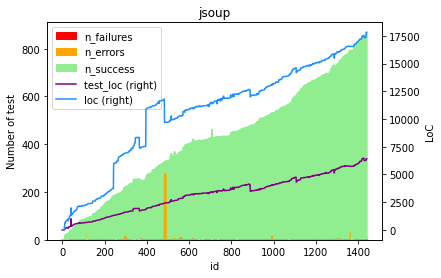
\includegraphics[width=\textwidth]{pages/02-Testability/images/projects/jsoup.png}
        \label{fig:jsoup}
    \end{minipage}%
    \begin{minipage}{.5\textwidth}
        \centering
        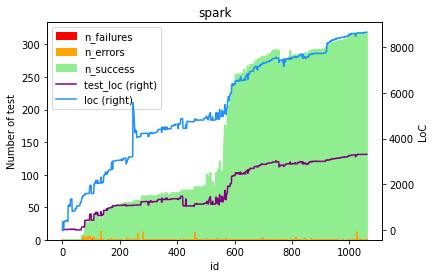
\includegraphics[width=\textwidth]{pages/02-Testability/images/projects/spark.png}
        \label{fig:spark}
    \end{minipage}
    \begin{minipage}{.5\textwidth}
        \centering
        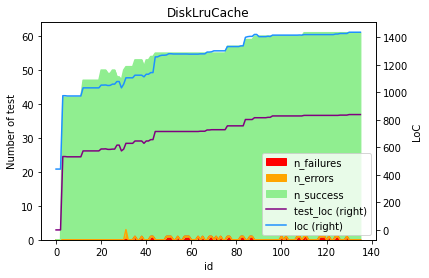
\includegraphics[width=\textwidth]{pages/02-Testability/images/projects/disklrucache.png}
        \label{fig:disklrucache}
    \end{minipage}%
    \caption{Set of projects 1: DiskLRUCache, Spark and JSoup}
    \label{fig:projects-1}
\end{figure}

\begin{table}[h!]
    \centering
    \resizebox{\textwidth}{!}{%
        \begin{tabular}{|r|r|r|r|}
        \hline
        \textbf{Project} & \textbf{Src Compilability}  & \textbf{Test Compilability} & \textbf{Fully Testability} \\ \hline
        jsoup            &  97.87\%                       & 97.29\%                      & 93.55\%                      \\ \hline
        spark            &  98.96\%                       & 92.84\%                      & 86.72\%                      \\ \hline
        DiskLruCache     &  100.00\%                      & 97.79\%                      & 70.58\%                      \\ \hline
        \end{tabular}
    }
    \caption{Metrics of set of projects 1: JSoup, Spark and DiskLRUCache}
    \label{table:projects-1}
\end{table}

%%%%%%%%%%%%%%%%%%%%%%%%%%%%%%%%%%%%%%%%%%%%%%%%%%%%%%%%%%%%%%%%%%%%%
%                           SECOND SET                              %
%%%%%%%%%%%%%%%%%%%%%%%%%%%%%%%%%%%%%%%%%%%%%%%%%%%%%%%%%%%%%%%%%%%%%

The second set of project that we are going to study (Figure~\ref{fig:projects-2}) have been selected as a representative set of projects that, taking a look at their visual representation, it seems that it is possible to run the tests in the past in almost all their history, although in some of them we find multiple commits where failures or errors are located.
However, if we look again at the Fully Testability values (Table~\ref{table:projects-2}), we find that their values are surprisingly low. 
For example, the \textit{Checkstyle} project, despite the fact that a portion of its commits at the beginning of the project are not compilable, the figure seems to indicate that almost all of its tests pass. 
Its low Fully Testability value is due to a few tests fail\patxi{failing consistently (in the order of 10 out of 1000)?}\michel{Como en la figura se muestra la cantidad de test verdes/rojos que hay, se puede apreciar que en la mayoria de commits el \% es muy bajo, menos de 10 por cada 1000} along the project history.
% \michel{He vuelto a mirar muy en detalle, parece que al re-ejecutarlo han cambiado un poco los resultados. En un párrafo no puedo comentarte exacatemente lo que he encontrado. Tengo que enseñarte las tablas y comentarte. Rápidamente puedo decir que en este proyecto solo pasan los test en el 0.01\% de los commtis (81). En la mayoria de commits, un porcentaje muy bajo de test fallan. En un commit en concreto fallan 17 test, pero en los demás es menos de 10 (con +1000 test). Hay test que fallan en todos los commits, pero no son muchos (17 test únicos). Hay un par de test más que fallan en muy pocos commits. Para ver los logs de porqué fallan esos test tengo que bajarme los resultados de Minio y descomprimirlos, por lo que me gustaría comentarlo antes}
The other two projects expose a similar behavior, in the case of \textit{HikariCP} the failures are more visible in the graph (there are more tests per commit resulting in failures or errors) despite having the highest Fully Testability value of this set.

\begin{figure}[!htb]
    \centering
    \begin{minipage}{.5\linewidth}
        \centering
        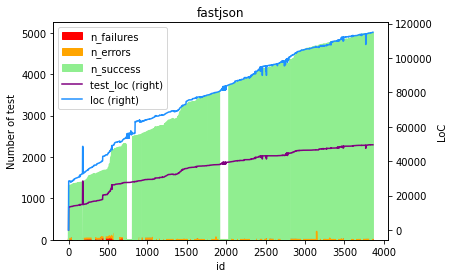
\includegraphics[width=\textwidth]{pages/02-Testability/images/projects/fastjson.png}
        \label{fig:fastjson}
    \end{minipage}%
    \begin{minipage}{.5\linewidth}
        \centering
        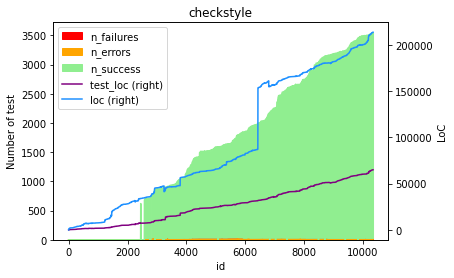
\includegraphics[width=\textwidth]{pages/02-Testability/images/projects/checkstyle.png}
        \label{fig:checkstyle}
    \end{minipage}
    \begin{minipage}{.5\linewidth}
        \centering
        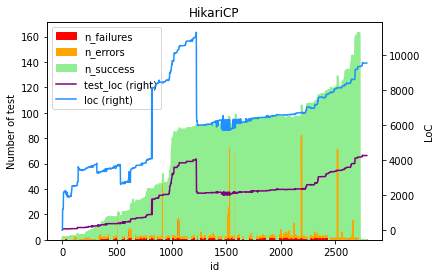
\includegraphics[width=\textwidth]{pages/02-Testability/images/projects/hikari.png}
        \label{fig:hikari}
    \end{minipage}%
    \caption{Set of projects 2: Fastjson, Checkstyle and HikariCP}
    \label{fig:projects-2}
\end{figure}

\begin{table}[h!]
    \centering
    \resizebox{\textwidth}{!}{%
        \begin{tabular}{|r|r|r|r|}
        \hline
        \textbf{Project} & \textbf{Src Compilability} & \textbf{Test Compilability} & \textbf{Fully Testability} \\ \hline
        HikariCP         &  96.02\%                      & 95.22\%                      & 16.92\%                      \\ \hline
        Checkstyle       &  77.72\%                      & 74.35\%                      & 0.78\%                      \\ \hline
        Fastjson         &  94.25\%                      & 88.35\%                      & 0.00\%                      \\ \hline
        \end{tabular}
        }
    \caption{Metrics of set of projects 1: Fastjson, Checkstyle and HikariCP}
    \label{table:projects-2}
\end{table}

Considering the above-mentioned results, Fully Testability is a very restrictive metric, as soon as a single test does not pass consistently in several commits, it drastically reduces the value of the metric. 
We can consider that we are missing information about the real testability of the project.
From the point of view of a practitioner or a researcher who needs to add a change to a past version and has to evaluate if the tests allow him to be sure not to introduce any regression in the code, knowing that in a commit 99.99\% of the tests pass may be enough.
This happened in the case of the \textit{Checkstyle} project, where there are commits with 3506 tests but only 1 fails.
\patxi{Esta frase es muy larga pero no sé cómo partirla.}
\michel{He sacado el texto del parentesis (el ejemplo) como una nueva frase para aligerlo un poco.}

Following this discussion, we propose a new and less restrictive way of measuring testability, which allows us to capture the information in a non-binary way. 
Instead of using a binary value (a commit is either Fully Testable or not) we will use a ratio. 
Hence, a commit has a \textbf{Testable Rate}, defined as the ratio of success tests with respect to the total number of tests run for that commit.
For a project, we would obtain the \textbf{Testability Rate} as the mean of the Testable Rate value of all commits in the history.

Table~\ref{table:projects-2-with-testability-rate} shows the Testability Rate results for the second set of projects.
This new metric reflects a higher testability value for this set of projects, which is in line with the reality of the tests executed.

\begin{table}[h!]
    \centering
    \resizebox{\textwidth}{!}{%
        \begin{tabular}{|r|r|r|r|r|}
        \hline
        \textbf{Project} & \multicolumn{1}{c|}{\textbf{\begin{tabular}[c]{@{}c@{}}Src \\ Compilability\end{tabular}}} & \multicolumn{1}{c|}{\textbf{\begin{tabular}[c]{@{}c@{}}Test \\ Compilability\end{tabular}}} & \multicolumn{1}{c|}{\textbf{\begin{tabular}[c]{@{}c@{}}Fully\\ Testability\end{tabular}}} & \multicolumn{1}{c|}{\textbf{\begin{tabular}[c]{@{}c@{}}Testability\\ Rate\end{tabular}}} \\ \hline
        HikariCP         &  96.02\%                      & 95.22\%                      & 16.92\%                      & 88.76\%                     \\ \hline
        checkstyle       &  77.72\%                      & 74.35\%                      & 0.78\%                       & 74.22\%                     \\ \hline
        fastjson         &  94.25\%                      & 88.35\%                      & 0.00\%                       & 87.80\%                     \\ \hline
        \end{tabular}
    }
    \caption{Metrics of set of projects 1: Fastjson, Checkstyle and HikariCP (including the new Testability Rate metric)}
    \label{table:projects-2-with-testability-rate}
\end{table}

%%%%%%%%%%%%%%%%%%%%%%%%%%%%%%%%%%%%%%%%%%%%%%%%%%%%%%%%%%%%%%%%%%%%%
%                            THIRD SET                              %
%%%%%%%%%%%%%%%%%%%%%%%%%%%%%%%%%%%%%%%%%%%%%%%%%%%%%%%%%%%%%%%%%%%%%

The third set of projects is shown in Figure~\ref{fig:projects-3}. 
In this case, we have chosen projects that appear to be very testable but only in a part of their history (due to problems in compiling the source code or test code).
Table~\ref{table:projects-3} shows the testability values for these projects. 

\begin{figure}[!htb]
    \centering
    \begin{minipage}{.5\linewidth}
        \centering
        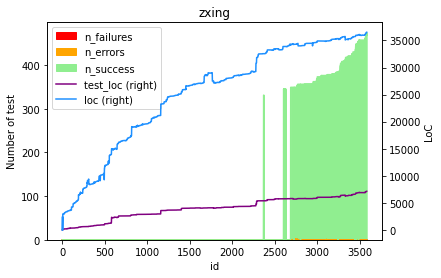
\includegraphics[width=\textwidth]{pages/02-Testability/images/projects/zxing.png}
        \label{fig:zxing}
    \end{minipage}%
    \begin{minipage}{.5\linewidth}
        \centering
        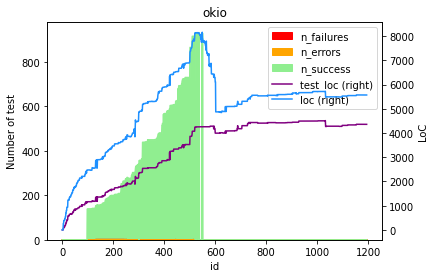
\includegraphics[width=\textwidth]{pages/02-Testability/images/projects/okio.png}
        \label{fig:okio}
    \end{minipage}
    \begin{minipage}{.5\linewidth}
        \centering
        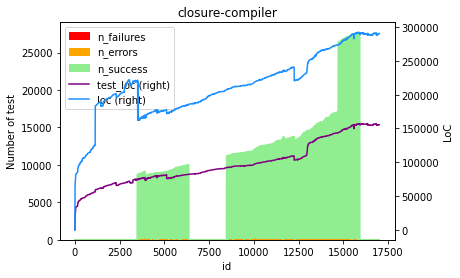
\includegraphics[width=\textwidth]{pages/02-Testability/images/projects/closure.png}
        \label{fig:closure-compiler}
    \end{minipage}%
    \caption{Set of projects 3: Zxing, Okio and Closure}
    \label{fig:projects-3}
\end{figure}

\begin{table}[h!]
    \centering
    \resizebox{\textwidth}{!}{%
        \begin{tabular}{|r|r|r|r|r|}
            \hline
            \textbf{Project} & \multicolumn{1}{c|}{\textbf{\begin{tabular}[c]{@{}c@{}}Src \\ Compilability\end{tabular}}} & \multicolumn{1}{c|}{\textbf{\begin{tabular}[c]{@{}c@{}}Test \\ Compilability\end{tabular}}} & \multicolumn{1}{c|}{\textbf{\begin{tabular}[c]{@{}c@{}}Fully\\ Testability\end{tabular}}} & \multicolumn{1}{c|}{\textbf{\begin{tabular}[c]{@{}c@{}}Testability\\ Rate\end{tabular}}} \\ \hline
            okio             & 36.65 & 36.06\%                      & 26.27\%                       & 36.01\%                     \\ \hline
            closure          & 60.18 & 59.84\%                      & 55.81\%                       & 59.84\%                     \\ \hline
            zxing            & 25.47 & 25.39\%                      & 24.80\%                       & 25.38\%                     \\ \hline
        \end{tabular}
    }
    \vspace*{0.5cm}
    \captionof{table}{Metrics of set of projects 3: Zxing, Okio and Closure}
    \label{table:projects-3}
\end{table}

These projects are characterized by a low Test Compilability. 
The Test Compilability metric is greatly affected by Source Compilability; if the code does not compile, the tests cannot be compiled. 
The reasons why source code cannot be compiled have been studied in previous chapter and in previous work~\cite{tufano2017there,Sulir:2016:QSJ:3001878.3001882}, and are caused mainly because of the impossibility to reproduce the context and retrieve the dependencies of a particular commit. 
For the okio, closure and zxing projects, the Source Compilability values are very close to Test Compilability values.
So, we can state that in these projects, if the source code compiles, in most cases the test code compiles as well. 
We can reflect this in a new metric: Test Compilability\textsubscript{S}, the ratio of test-compilable commits with respect to the source-compilable commits.
The Test Compilability metric, when calculated considering all commits in the project history, is renamed to Test Compilability\textsubscript{A}.
Table~\ref{table:projects-3-B} shows the values of these two variants of Test Compilability, in addition to the Source Compilability values mentioned above.


\begin{table}[h!]
    \centering
    \resizebox{\textwidth}{!}{%
        \begin{tabular}{|r|r|r|r|r|r|}
        \hline
        \multicolumn{1}{|c|}{\textbf{Project}} & \multicolumn{1}{c|}{\textbf{\begin{tabular}[c]{@{}c@{}}Src \\ Compilability\end{tabular}}} & \multicolumn{1}{c|}{\textbf{\begin{tabular}[c]{@{}c@{}}Test \\ Compilability\textsubscript{A}\end{tabular}}} & \multicolumn{1}{c|}{\textbf{\begin{tabular}[c]{@{}c@{}}Test \\ Compilability\textsubscript{S}\end{tabular}}} & \multicolumn{1}{c|}{\textbf{\begin{tabular}[c]{@{}c@{}}Fully\\ Testability\end{tabular}}} & \multicolumn{1}{c|}{\textbf{\begin{tabular}[c]{@{}c@{}}Testability\\ Rate\end{tabular}}} \\ \hline
        okio                                   & 36.65\%                                                                                        & 36.07\%                                                                                         & 98.40\%                                                                                         & 26.28\%                                                                                     & 36.02\%                                         \\ \hline
        closure                                & 60.18\%                                                                                        & 59.84\%                                                                                         & 99.43\%                                                                                         & 55.82\%                                                                                     & 59.84\%                                         \\ \hline
        zxing                                  & 25.47\%                                                                                        & 25.39\%                                                                                         & 99.67\%                                                                                         & 24.80\%                                                                                     & 25.39\%                                         \\ \hline
        \end{tabular}
    }
    \captionof{table}{Extended metrics of set of projects 3: Zxing, Okio and Closure}
    \label{table:projects-3-B}
\end{table}

Following the idea of focusing on those commits where we can compile the test code, we should consider that it is possible that the commits that do not compile, never did and therefore their testability information is not useful to us.
% Once again we find that the testability metrics do not provide all the information. 
% When we cannot compile source code or test code, we lose testability information. 
For projects such as those in set 3, the testability of the commits where we can compile the tests gives us valuable information that neither the Fully Testability nor the Testability Rate capture, as both metrics are calculated from all commits in the history of the project.

To capture the testability of Test Compilable commits we define the following metrics:
\begin{itemize}
    \item \textbf{Testability Rate\textsubscript{T}}: mean of \textit{testable rate} for \textit{test-compilable commits} in the project.
    \item \textbf{Fully Testability\textsubscript{T}}: ratio of \textit{fully testable commits} with respect to the number of \textit{test-compilable commits} of the project.
\end{itemize}
The Fully Testability and Testability Rate metrics, when calculated considering all the commits in the history, are renamed Fully Testability\textsubscript{A} and Testability Rate\textsubscript{A}.

In Table~\ref{table:projects-3-with-flavor-testability-rate} we include the new metrics defined for the third set of projects. 
We note that for all 3 projects, the new metrics more closely capture the testability of the commits we can compile.
The Fully Testability\textsubscript{T} shows us that for those commits where we can compile the tests, a high percentage can run all their tests with a success result. For this same set of commits, the Testability Rate\textsubscript{T} shows us values close to 100\%; almost all of the tests in these commits offer a success result.

\begin{table*}[h!]
    \centering
    \resizebox{\textwidth}{!}{%
        \begin{tabular}{|r|r|r|r|r|r|r|r|}
            \hline
            \rH{Project} & \rH{Src\\ Compilability} & \rH{Test\\ Compilability\textsubscript{A}} & \rH{Test\\ Compilability\textsubscript{S}} & \rH{Fully\\Testability\textsubscript{A}} & \rH{Fully\\Testability\textsubscript{T}} & \rH{Testability\\Rate\textsubscript{A}} & \rH{Testability\\Rate\textsubscript{T}} \\ \hline
            okio             & 36.65\%                        & 36.07\%                         & 98.40\%                         & 26.28\%                        & 72.85\%                        & 36.02\%                       & 99.86\%                       \\ \hline
            closure          & 60.18\%                        & 59.84\%                         & 99.43\%                         & 55.82\%                        & 93.27\%                        & 59.84\%                       & 99.99\%                       \\ \hline
            zxing            & 25.47\%                        & 25.39\%                         & 99.67\%                         & 24.80\%                        & 97.69\%                        & 25.39\%                       & 100.00\%                      \\ \hline
        \end{tabular}
    }
    \caption{Extended metrics of set of projects 3: Zxing, Okio and Closure (including the new Testability Rate\textsubscript{T} and Fully Testability\textsubscript{T} metrics)}
    \label{table:projects-3-with-flavor-testability-rate}
\end{table*}

%\patxi{Podría ser interesante incluir también o analizar los del conjunto 1, para dar una idea de la robustez de esta métrica: ¿sigue manteniéndose alta en el primer conjunto de proyectos y refleja por tanto lo que queremos?}
%\michel{Temo sobrecargar esta sección de tablas. Mi impresión es que las métricas son esperables teniendo en cuenta los razonamientos que hemos hecho, no aportan nada nuevo.}

\def \RQIII{How many tests of a snapshot can be run with a `success' result?}

This case study helped us to define metrics that better describe a project's stability. These new metrics lead to a new research question: 

\textbf{RQ\textsubscript{3}}: ``\RQIII''
\michel{Habría quedar una vuelta a la pregunta}
\patxi{Yo diría: For those commits of a project on which tests compile, how many of them can be run with a success result?}
\michel{To discuss: Ojo cuidado, que la pregunta deberia ser para todos los commits, no solo para los compilables. (No lo digo yo, este comentario lo ha generado Copilot :D). Solo los compilables es la TestabilityRate_T}

\section{Experimental results}
\label{sec:testability:results}
Once we performed our case study and determined the metrics that might better represent the projects, in this section we resort to describe the results in detail using the metrics defined in the previous section.

After running the experiment, we detected 20 projects in which not a single test was run on any commit in the history. 
The learning-spark project does not contain any tests in any commit of its history. 
The Mycat-Server project has a dependency on software that must be installed on the machine for it to be compiled (therefore its Source Compilability is 0\%). 
The Clojure project is a programming language and as such, its tests require a different execution method. 
The remaining 17 projects correspond to projects that contain multiple Maven modules and cannot be compiled and tested with the proposed methodology. 
\patxi{Ojo con esto que nos pueden decir que lo arreglemos, que un proyecto maven multimodulo no es nada raro}
\michel{Tenemos algunos proyectos multi-modulo que sí se pueden construir y testear con la metodología propuesta.}
%Despite the interest and the percentage of the total that these projects represent, we consider that they should be studied in a separate study. \patxi{Yo quitaba esta frase.}
Since we cannot execute any of the tests on any of these projects, we have decided to leave them out of our study, and from this point on we will only consider the remaining 66 projects.

Table~\ref{table:results-1} shows a summary of the experiment for the 66 projects. 
In the Count column we can see the magnitude of the study for the metrics defined in the methodology. 
The Mean ({\large$\mean{x}$}) and Median ({\large$\median{x}$}) columns show the trend at the project level.
We run a normality test for each metric in this table, finding that with the exception of \textit{Age}, none of the metrics shows a normal distribution. 
In general, differences between mean and median show large internal variability in each of the samples.

\begin{table}[!htb]
    \centering
    \caption{Absolute results.}
    \label{table:results-1}
    \begin{tabular}{|r|r|r|r|}
        \hline
        \multicolumn{1}{|c|}{\textbf{Metric}}& \multicolumn{1}{c|}{\textbf{Count}} & \multicolumn{1}{c|}{\textbf{\large{$\mean{x}$}}} & \multicolumn{1}{c|}{\textbf{\large{$\median{x}$}}} \\ \hline
        \textbf{Age}                      & 634.66                              & 9.62                               & 9.69                                 \\ \hline
        \textbf{LoC}                      & 11,143,058                         & 174,110.28                          & 26,973.50                             \\ \hline
        \textbf{Commits}                  & 407,579                           & 6,175.44                            & 2,831.00                              \\ \hline
        \textbf{Source-compilable commits} & 103,097                           & 1,562.08                            & 1,020.00                              \\ \hline
        \textbf{Test-compilable commit}    & 93,925                            & 1,423.11                            & 692.50                               \\ \hline
        \textbf{Fully Testable commits}   & 40,540                            & 614.24                             & 218.00                               \\ \hline
    \end{tabular}
\end{table}

Table~\ref{table:results-3} shows information on the compilability and testability metrics of the projects of the dataset. 
\patxi{Esta línea huérfana aquí se queda muy pobre. Habría que explicarlo un poco más.}
\michel{El problema aquí es que estos resultados se discuten en la siguiente sección. ¿Deberías fusionar ambas secciones?}

\begin{table}[h]
    \centering
    \caption{Mean ($\mean{x}$) and Median ($\median{x}$) values for Compilability and Testability of the projects.}
        \label{table:results-3}
        \begin{tabular}{|r|r|r|}
            \hline
            \multicolumn{1}{|c|}{\textbf{Metric}} & \multicolumn{1}{c|}{\textbf{Mean}} & \multicolumn{1}{c|}{\textbf{Median}} \\ \hline
            \textbf{Source Compilability}                         & 47.29\%                              & 47.12\%                                \\ \hline
            \textbf{Test Compilability\textsubscript{A}}          & 41.73\%                              & 39.22\%                                \\ \hline
            \textbf{Test Compilability\textsubscript{S}}          & 88.26\%                              & 97.35\%                                \\ \hline
            \textbf{Testability Rate\textsubscript{A}}           & 38.63\%                              & 34.88\%                                \\ \hline
            \textbf{Testability Rate\textsubscript{T}}           & 94.14\%                              & 99.53\%                                \\ \hline
            \textbf{Fully Testability\textsubscript{A}}          & 22.12\%                              & 14.88\%                                \\ \hline
            \textbf{Fully Testability\textsubscript{T}}          & 52.53\%                              & 59.32\%                                \\ \hline
    \end{tabular}
\end{table}


To illustrate the diversity of the results, we have divided the 66 projects into three groups of the same size according to their number of commits: large, medium and small. 
Figures~\ref{fig:many4j-1-bar-chart} (large projects), \ref{fig:many4j-2-bar-chart} (medium projects) and \ref{fig:many4j-3-bar-chart} (short projects) show the results for each project for each of the integer metrics as overlapping bars.
\patxi{Primero di que los agrupas por número de commits, y luego explicas lo de las barras. SI no queda raro}
\michel{Hecho}
% To illustrate the diversity of results across the projects, we have represented the different categories of commits per project in overlapped bars in Figures~\ref{fig:many4j-1-bar-chart} (large projects), \ref{fig:many4j-2-bar-chart} (medium projects) and \ref{fig:many4j-3-bar-chart} (short projects).
% The division of projects into the three categories (long, medium and short) is based on the number of commits.
It is easy to appreciate, just by checking colors, how each project tells a very different story. 

\begin{figure}[h!]
    \centering    
    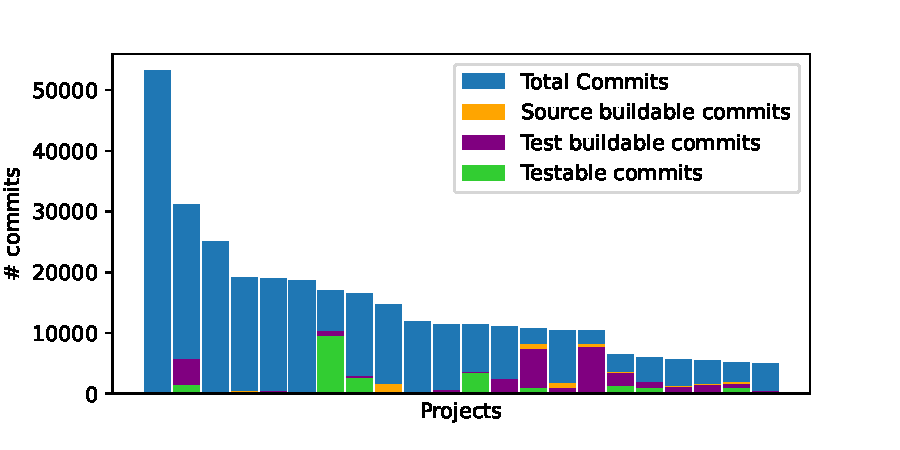
\includegraphics[width=0.8\textwidth]{pages/02-Testability/images/Many4j 1-22.pdf}
    \caption{Project metrics (Large projects)}
    \label{fig:many4j-1-bar-chart}
\end{figure}%
\begin{figure}[h!]
    \centering    
    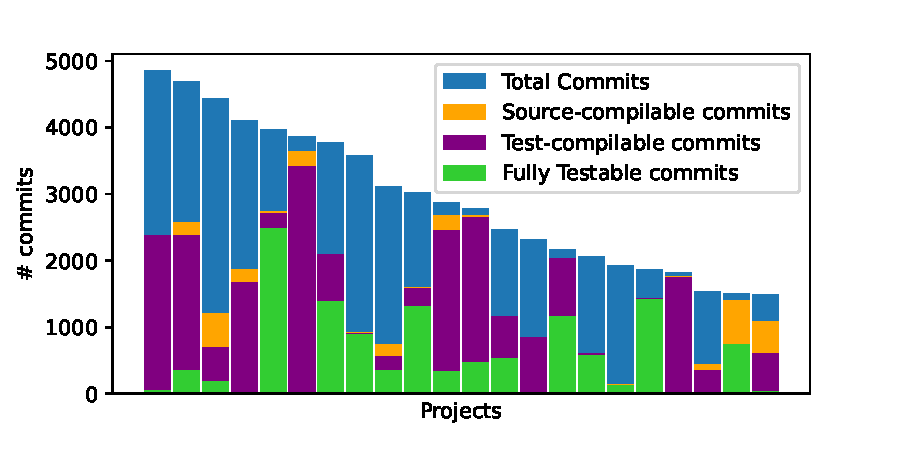
\includegraphics[width=0.8\textwidth]{pages/02-Testability/images/Many4j 23-44.pdf}
    \caption{Project metrics (Medium projects)}
    \label{fig:many4j-2-bar-chart}
\end{figure} 
\begin{figure}[h!]
    \centering    
    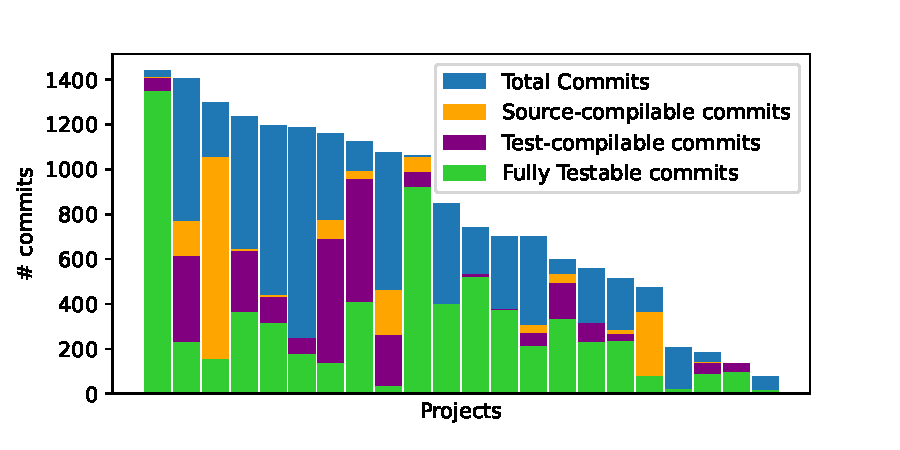
\includegraphics[width=0.8\textwidth]{pages/02-Testability/images/Many4j 45-66.pdf}
    \caption{Project metrics (Short projects)}
    \label{fig:many4j-3-bar-chart}
\end{figure}

\section{Analysis}
\label{sec:testability:analysis}
Let's now analyze in some more detail some \patxi{the} results presented in the previous section.

The mean \textbf{Source Compilability} of the projects (47.29\%), although low, is slightly higher than in previous studies on Java projects such as that of Tufano et al (38.13\%). 
This is partly due to having left out 20 projects whose compilability was 0.
But what is more interesting is the differences from project to project, something that was expected, and seen in previous studies on the matter~\cite{tufano2017there,sulir2020large,querel:2021:warning}.

The mean value of the \textbf{Test Compilability\textsubscript{A}} is significantly lower (41.73\%), because Source Compilability is a threshold for this metric.
Moreover, considering only those commits where the source code is compiled, the \textbf{Test Compilability\textsubscript{S}} offers a considerably higher value on average (88\%).
This value is reasonable, since once the main source code was built \patxi{compile?}, it is more likely that the test code can also be built\patxi{compile? Revisar todos los build y built}. 
% What is maybe unexpected, as we will discuss later in Section~\ref{sec:semantics}, is that it is not even higher.
We also note that for this metric, 50\% of the projects offer a value higher than 97\%.\patxi{Therefore, test compilation does not seem a problem in general, and efforts, in any case, should be put in source compilation.}


%In contrast, it seems that the compilability of both source code and tests is significantly lower than for projects collected through the GitHub API. Many4J projects offer a significantly lower mean on all parameters.

The most clear result when analyzing testability of projects is its variability from project to project. 
Figure~\ref{fig:testability-overview} illustrates this, by showing the shape of the distribution of all testability metrics we defined, for all projects.

\begin{figure*}[ht!]
    \centering    
    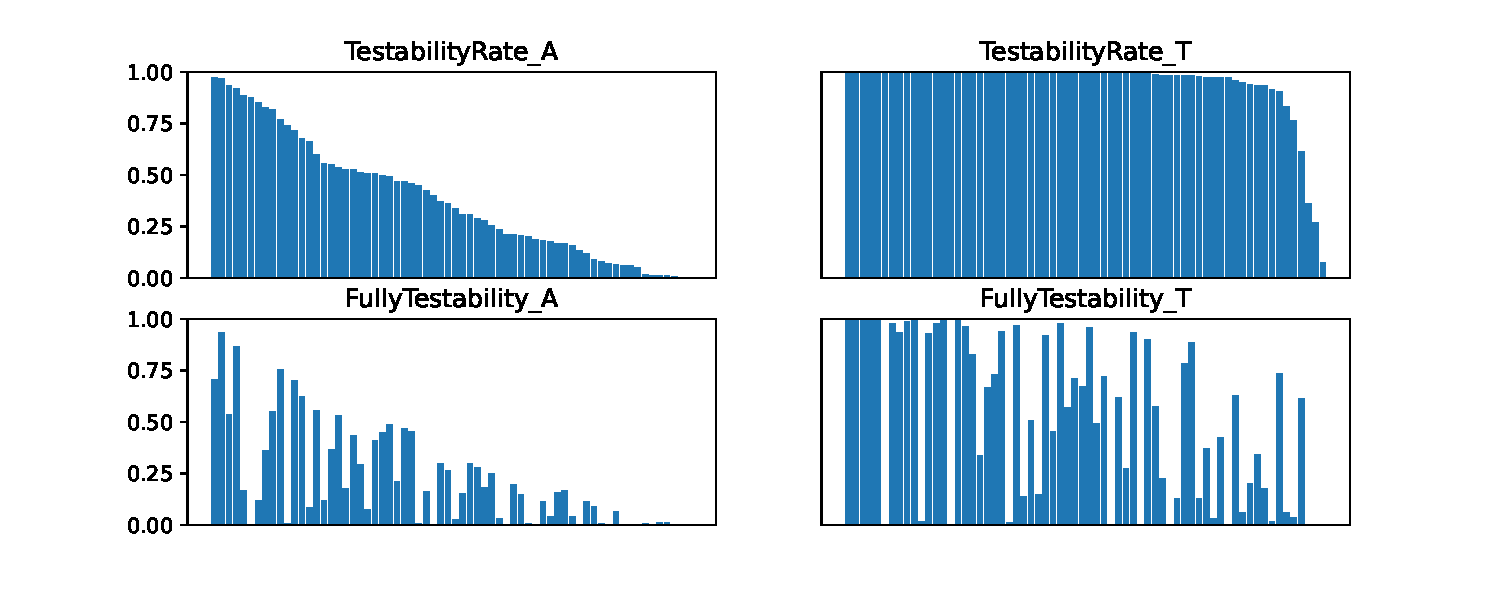
\includegraphics[width=\textwidth]{pages/02-Testability/images/Overview.pdf}
    \caption{Overview of testabilities - Each bar represents a project. Each column\patxi{column? Hay que ver cómo decir esto que se entienda mejor} is ordered by the corresponding Testability Rate (A and T) of each project.}
    \label{fig:testability-overview}
\end{figure*}

Looking at the Testability Rate values, when we focus on those commits where the tests can be built (\textbf{Testability Rate\textsubscript{T}}) we observe an average value of 94.14\%, a high percentage of the project's tests are executed successfully. 
% Again, we see that the \textbf{Testability Rate\textsubscript{T}}, as with other values, varies a lot between projects, with the median of this value being 99.53\%, indicating that in 50\% of the cases almost all the tests pass for test compilable commits.
By calculating the Testability Rate considering all commits (\textbf{Testability Rate\textsubscript{A}}), this value gives an overview of the testability of the project and how Source Compilability impacts running tests on past commits.

Focusing on \textbf{Fully Testability\textsubscript{T}}, we could expect it would be usually high: developers should write code that does not break \textit{all} the tests. 
Fact is that in more than half of the commits that were test-compilable some tests fail when they are run. 
This result, which may seem surprising, deserves as well more discussion that we will provide in Section~\ref{sec:low-testability}.\patxi{¿Por qué no aquí si estamos en la sección de análisis?}

\textbf{Fully Testability\textsubscript{A}} gives quite interesting information: the fraction of commits that are testable, with respect to the total number of commits. 
When compilability is low, this fraction is necessarily low, just meaning that commits are not testable because they are not source- or test-compilable. 
When compilability is high, \textit{Fully Testability\textsubscript{A}} really shows differences.\patxi{¿Qué diferencias¿Entre proyectos? -> among projects} 

With the data presented up to here, we can already answer RQ\textsubscript{1}, RQ\textsubscript{2} and RQ\textsubscript{3}\patxi{Ojo, la numeración de las RQs ha cambiado: 2.1, 2.2, 2.3, y en los siguientes párrafos igual}:

\vspace{0.5cm}
\fbox{\begin{minipage}{\textwidth}
\textbf{\textbf{RQ\textsubscript{1}}: ``\RQI''}
We found 93,925 test-compilable commits out of 103,097 source-compilable commits.
When calculating \textit{Test Compilability} using all the commits of the project we obtain an average value of 41.73\%, while if we compute only the commits in which we can compile the source code, the average value increases significantly (88.2\%).\patxi{Hay que aportar algo más aquí que sólo los datos. ¿Qué implica esto?: We can conclude that when the source code compiles, the test code compile, therefore, in general, test compilation is not an issue.}
\end{minipage}}

\vspace{0.5cm}
\fbox{\begin{minipage}{\textwidth}
\textbf{\textbf{RQ\textsubscript{2}}: ``\RQII''}
We found 40,540 fully-testable commits out of 93,925 test-compilable commits. 
When calculating \textit{Fully Testability} using all the commits of the project we obtain an average value of 22.12\%, while if we compute only the commits in which we can compile the tests, the average value increases significantly (52.53\%).\patxi{This is quite surprising, as one would expect that all tests should pass before a commit is accepted (after all, this is what CI is for). The results that we show here indicates that this is not always the case. We discuss it further in the next section.}
\end{minipage}}

\vspace{0.5cm}
\fbox{\begin{minipage}{\textwidth}
\textbf{\textbf{RQ\textsubscript{3}}: ``\RQIII''}
When calculating \textit{Testability Rate} using all the commits of the project we obtain an average value of 38.63\%, while if we compute only the commits in which we can compile the tests, the average value increases significantly (94.14\%).\patxi{This is in line with our expectations: in general when the tests compile, they succeed.}
\end{minipage}}
    


\section{Discussion}
\label{sec:testability:discussion}
After presenting the main results, and its analysis, in this section we discuss some details of our studies, including the threats to their validity.
%In conducting the different studies, we have found that there is a great variety in the testability of the different projects, even within the same study. In this section we will discuss the semantics of the testability metrics, analyse some of the projects with the higher testability, study why projects have low testability and, finally, present the  threats to validity of this work.

\michel{Aqui faltan dos subsecciones: una sobre la semantica de las metricas, y otra sobre los proyectos con alta testabilidad. La primera queda bastante obsoleta con el CaseStudy, la segunda tendría que volver a escribirla, ya que las métricas no son las mismas}

% \subsection{On the semantics of testability metrics}
% \label{sec:semantics}

% \michel{Es posible que esta sub-sección, con el nuevo Case Study, no tenga mucho sentido}

% For the studies presented in this paper, we designed a framework based on extending buildability to consider also buildability of tests, and introducing four \textit{Testability} metrics. 
% Each of these metrics shows a different aspect of testability.

% In continuous integration systems it is common that all tests must pass, being the result of their execution a binary value: either all tests pass or all tests fail. 
% In this context, we define that a commit is FullyTestable if all tests are success. 
% At the project level, we can identify how many commits are FullyTestable and provide a metric representing their percentage (Fully Testability). 
% It is common to consider all the commits of a project to calculate this type of metric.
% \textit{Fully Testability\textsubscript{A}} could be considered the ``absolute'' testability, since it considers all commits.
% In a project with 100\% \textit{Fully Testability\textsubscript{A}} all past snapshots are testable. 
% However, there are constraints, not related to the tests themselves, that put limits to testability.
% For example, a test that cannot be built, cannot be run. 
% Therefore, we defined \textit{Fully Testability\textsubscript{T}} to capture these constraints, and define testability related to them. 
% They inform on the quality of the tests only for snapshots that are buildable (either source- and tests-buildable). 
% In more detail:

% \begin{itemize}
%     \item \textbf{A high \textit{Fully Testability\textsubscript{A}}} signals a \textbf{highly reproducible project}: most of its snapshots are buildable, and the execution of their tests is successful.
%     The project in our dataset with the highest value in this metric is \textit{jsoup}, with a value of 93.55\%. 
%     This project, and others with high \textit{Fully Testability\textsubscript{A}}, are analyzed in the section~\ref{sec:high}.
%     \item \textbf{A high \textit{Fully Testability\textsubscript{T}}} hints to a project with \textbf{highly reproducible execution of tests}: most tests that can be built can also be executed successfully. 
%     A good example is \textit{JFinal}, with a value of 100\%. 
%     Its low \textit{Test Buildability} (22\%) considerably affects its \textit{Fully Testability\textsubscript{B}} (22\%). 
%     In this case, \textit{Fully Testability\textsubscript{T}} shows that as long as the tests are built correctly, they can be executed successfully. 
%     In projects with high \textit{Fully Testability\textsubscript{T}} and low \textit{Test Buildability} it is reasonable to think that improving \textit{Test Buildability} could increase also \textit{Fully Testability\textsubscript{A}}.
% \end{itemize}

% There are some projects as well with a high percentage of tests executed successfully, but low \textit{Fully Testability}. 
% This is possible when many tests in a snapshot are executed successfully, but a few do not. 
% For example, Figure~\ref{fig:checkstyle} shows a stacked area chart of the test results for all snapshots of \textit{Checkstyle}: snapshots are in the X axis, and the number of tests for each of them in the Y axis. Most of the tests for each snapshot are green (test success), but there is a small orange area close to the X axis corresponding to tests executed with error. 
% Due to these errors, most of the commits are not testable, and the project has a very low \textit{Fully Testability\textsubscript{A}} (1\%). 
% The reason for this is binary definition for Fully Testability, based on the rule of ``all tests should pass''. 
% Even when it is useful to compare with the ideal situation, there is room for defining additional metrics that reflect the high reproducibility of the tests in projects like this.

% \begin{figure}[t]
%     \centering    
%     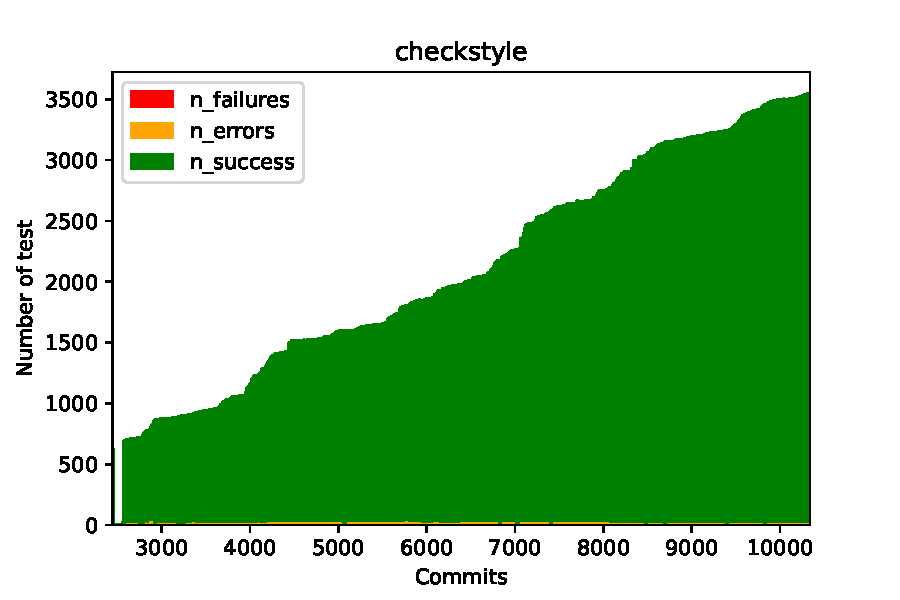
\includegraphics[width=8cm]{images/checkstyle.pdf}
%     \vspace{-0.2cm}
%     \caption{Tests results for Checkstyle project}
%     \label{fig:checkstyle}
% \end{figure}

% For this purpose, for each project commit, we define \textit{TestableRate}. 
% This value will show us the ratio of tests with a success result against the total number of tests of that commit. 
% In this way, \textit{TestableRate} gives us a more complete view of how the tests have behaved in a commit.
% Thus, a commit being \textit{FullyTestable} would only be a particular case where the value of \textit{TestableRate} is 100\%.

% In order to study the percentage of tests that pass at the project level, we find that it is difficult to capture in a metric that clearly reflects how the tests behave in the commit history. 
% The main limitation is when we consider all commits, since in those where the source code or test code cannot be built, we assume a TestableRate of 0\% because we do not know the real TestableRate.

% To illustrate it in an example, in Figure~\ref{fig:closure} we see the result of the tests in the history of the Closure project. 
% Several commits on its commit history cannot be built. 
% The mean TestableRate of all its commits is 59\%, while the median reaches 100\%.
% As in Fully Testability, in order to deal with the limitations of project buildability, Testability Rate C, B and T, considering all commits, source-buildable and test-buildable commits respectively, are defined in an analogous way.

% \begin{figure}[h]
%     \centering    
%     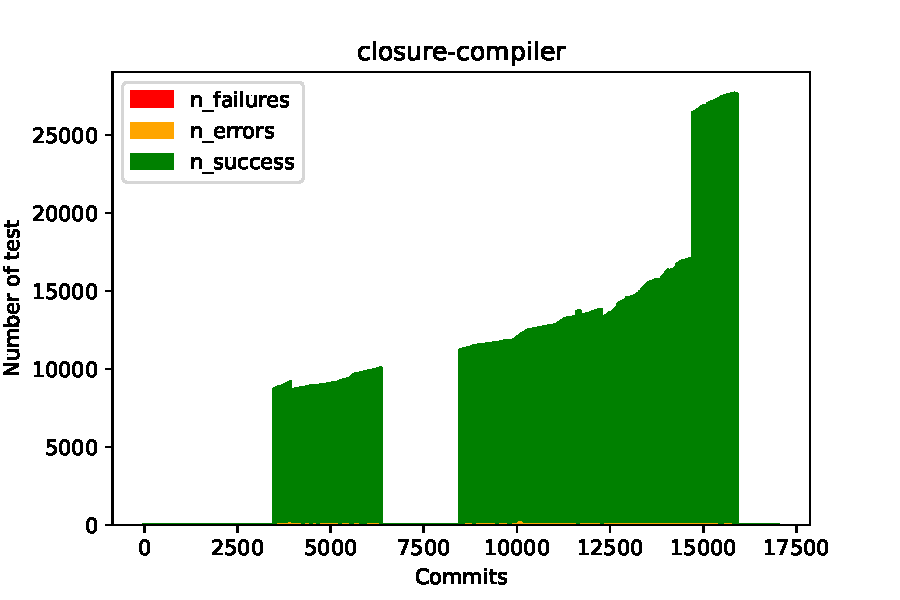
\includegraphics[width=8cm]{images/Closure.pdf}
%     \vspace{-0.2cm}
%     \caption{Tests results for Closure Compiler project}
%     \label{fig:closure}
% \end{figure}

% \subsection{Projects with high testability}
% \label{sec:high}

% We have identified some projects with high testability, which deserve a separate analysis. 
% To show these cases, we have searched for projects with the highest \textit{TestabilitRate} and the highest \textit{Fully Testability}.

% After analyzing the Testability Rate of the projects, we wanted to check which projects offer the highest results. Of the 86 projects:
% \begin{itemize}
%     \item We found 11 where the Testability Rate\textsubscript{A} is 100\% (i.e. in at least 50\% of their commits all the tests pass).
%     \item We found 39 where the Testability Rate\textsubscript{B} is 100\% (i.e. in at least 50\% of their source-buildable commits all the tests pass).
%     \item We found 44 where the Testability Rate\textsubscript{T} is 100\% (i.e. in at least 50\% of their test-buildable commits all the tests pass).
% \end{itemize}

% These values give us a very high number of projects, making an in-depth analysis difficult. 
% Therefore, in order to study projects with high testability, we have limited to those with high Fully Testability. 
% Specifically, we have selected the 3 projects that offer the best results for the different variants of Fully Testability (C, B and T).

% Tables~\ref{table:high-testability-A} and~\ref{table:high-testability-T} show metrics of the three projects with the highest Fully Testability of each flavor (A and T). 
% % La siguiente frase necesitaria más desarrollo
% %They could be good for identifying good practices that may help to increase testability of other projects.

% \begin{table}[h]
%     \centering
%     \caption{Top three projects with the highest \textit{Fully Testability\textsubscript{A}}}
%     \label{table:high-testability-A}
    
%     \begin{tabular}{|r|r|r|r|}
%         \hline
%         \textbf{Project}                  & \textbf{jsoup} & \textbf{spark} & \textbf{retrofit} \\ \hline
%         \textbf{Age}                      & 11.12          & 9.54           & 10.47         \\ \hline
%         \textbf{LoC}                      & 17,831         & 8,655          & 22,003           \\ \hline
%         \textbf{Total Commits}            & 1,442          & 1,062          & 1,865              \\ \hline
%         \textbf{Source buildable commits} & 1,410          & 1,051          & 1,431              \\ \hline
%         \textbf{Source buildability}      & 0.97           & 0.98           & 0.76          \\ \hline
%         \textbf{Test buildable commits}   & 1,403          & 986            & 1,431              \\ \hline
%         \textbf{Test buildability}        & 0.99           & 0.93           & 1.0               \\ \hline
%         \textbf{FullyTestable commits}    & 1349           & 921            & 1,411              \\ \hline
%         \textbf{Fully Testability\textsubscript{A}}      & \textbf{0.93} & \textbf{0.86} & \textbf{0.75} \\ \hline
%         \textbf{Fully Testability\textsubscript{B}}      & 0.95           & 0.87           & 0.98          \\ \hline
%         \textbf{Fully Testability\textsubscript{T}}      & 0.96           & 0.93           & 0.98          \\ \hline
%         \textbf{Testability Rate\textsubscript{A}}       & 1.0            & 1.0            & 1.0               \\ \hline
%         \textbf{Testability Rate\textsubscript{B}}       & 1.0            & 1.0            & 1.0               \\ \hline
%         \textbf{Testability Rate\textsubscript{T}}       & 1.0            & 1.0            & 1.0               \\ \hline
%     \end{tabular}
% \end{table}

% Among the projects with a high \textit{Fully Testability\textsubscript{A}} is \textit{jsoup}, a popular programming library for manipulating HTML code, which has only unit and integration tests.
% The second project, \textit{retrofit}, is a simple HTTP client, with the particularity that it is a multi-module project. 
% A high t\textit{Fully Testability\textsubscript{A}} C indicates that the tests of all its modules pass completely in most of the commits.
% All its tests use mocks, defined in its own module. 
% The robustness of testing functionality with mocks rather than with real endpoints (subject to change over time) may be one of the reasons for the good results of this project in this metric.
% The third project, \textit{spark}, is a lightweight web development framework. 
% It has end-to-end tests to verify the correct behavior when HTTP requests are performed; we have observed that these requests do not depend on remote services, though, which we have found in other projects to be a reason for low testability (see Section~\ref{sec:low-testability}).

% \begin{table}[h]
%     \centering
%     \caption{Top three projects with the highest \textit{Fully Testability\textsubscript{T}}}
%     \label{table:high-testability-T}
%     \begin{tabular}{|r|r|r|r|}
%         \hline
%         \textbf{Project}                  & \textbf{otto} & \textbf{javapoet} & \textbf{camel} \\ \hline
%         \textbf{Age}                      & 5.85          & 8.88              & 14.28          \\ \hline
%         \textbf{LoC}                      & 1,344        & 8,306            & 1,146,447      \\ \hline
%         \textbf{Total Commits}            & 205           & 846               & 53,286          \\ \hline
%         \textbf{Source buildable commits} & 18            & 398               & 21             \\ \hline
%         \textbf{Source buildability}      & 0.09          & 0.47              & 0.0            \\ \hline
%         \textbf{Test buildable commits}   & 18            & 396               & 20             \\ \hline
%         \textbf{Test buildability}        & 1.0           & 0.99              & 0.95           \\ \hline
%         \textbf{Fully Testable commits}   & 18            & 396               & 20             \\ \hline
%         \textbf{Fully Testability\textsubscript{A}}      & 0.09          & 0.47              & 0.0            \\ \hline
%         \textbf{Fully Testability\textsubscript{B}}      & 1.0           & 0.99              & 0.95           \\ \hline
%         \textbf{Fully Testability\textsubscript{T}}      & \textbf{1.0}  & \textbf{1.0}      & \textbf{1.0}   \\ \hline
%         \textbf{Testability Rate\textsubscript{A}}       & 0.0           & 0.0               & 0.0            \\ \hline
%         \textbf{Testability Rate\textsubscript{B}}       & 1.0           & 1.0               & 1.0            \\ \hline
%         \textbf{Testability Rate\textsubscript{T}}       & 1.0           & 1.0               & 1.0            \\ \hline
%     \end{tabular}
% \end{table}

% The three projects selected for the table with the highest \textit{Fully Testability\textsubscript{T}} are particularly interesting: whenever their tests could be constructed, they could be executed successfully. Two of them appeared in previous tables (\textit{otto} and \textit{javapoet}). The \textit{camel} project (a service integration library) offers a high \textit{Fully Testability\textsubscript{T}}, but this result must be considered in view of the fact that its buildability is only 0.03\%. For projects like this it is important to consider all \textit{Fully Testability} variants. 

\subsection{Why do projects have low testability?}
\label{sec:low-testability}

We have performed a preliminary study to identify the main reasons for some projects having low Fully Testability\textsubscript{A}. 
These reasons can be organized in three types:

\subsubsection{Low buildability.} 

\textit{Fully Testability\textsubscript{A}} of a project depends on the steps prior to the execution of the tests: building the main source code and the tests.
In projects with low buildability, testability is constrained by it.
Tufano et al. showed how one of the main reasons why a commit is no longer buildable is because of an error in obtaining the project dependencies~\cite{tufano2017there}. 
Therefore, it is possible that if those dependencies were available, the project not only built correctly, but also its tests could be executed successfully. 
We found several projects where the \textit{Fully Testability\textsubscript{A}} is low due to low buildability, but \textit{Fully Testability\textsubscript{B}} and \textit{Fully Testability\textsubscript{T}} are high.

\subsubsection{Snapshots were never testable.} When the project was being developed, not all of its commits were testable:

\begin{itemize}
    \item  \textbf{No tests in the snapshot}: 
    In some projects we have found no tests. 
    We consider these commits without test as non-testable, resulting in low values if many snapshots are like that.
    In these cases, maybe the project has tests, but they are not in the Maven project.
    \item \textbf{Snapshots with tests failing}: 
    When building and running tests on snapshots, we decided to try all of them in the master branch, since a recent study by Kovalenko et al.~\cite{kovalenko:2018:miningfilehistories} has shown that considering additional branches does not seem to have a significant impact compared to using only the master branch. 
    But depending on the strategy used by the developers to merge changes into master, we may find commits with tests failing even when they were merged. 
    For example, a commit includes a new feature which breaks some tests, but it is still merged, maybe because the next commit will fix the tests or the cause of the error.
    We found this case in \textit{elastic-job} by taking advantage of commit comments to understand the development workflow. 
    When refactoring, tests stop passing in some commits, being fixed in later commits (for example see commits 860, 929, 965, 1053 and 1120, where 0 is the last commit in the history).
    So, if some tests of a project were never testable, it is not possible to make the snapshot testable when reproducing the past.
\end{itemize}

\subsubsection{Context is not reproduced.} 
Without the right context, some tests cannot perform exactly as they did in the past. Here are some of the problems related to test execution context:

\begin{itemize}
    \item \textbf{Network services}: 
    In most of the integration test, the tests check how the software integrates with other network services. If these services need to be launched prior to running the tests, we will find connection-related exceptions when running the tests without the network services.
    A good example is the \textit{Jedis} project: it is a library for managing a Redis database. 
    If this database has not been launched when running the tests, the tests throw exceptions such as ``ConnectException'' or ``ConnectionRefused''.
    To address this type of problem, a good practice would be for the test itself to be able to launch the necessary context to be able to be executed.
    \item \textbf{Command line tools}: 
    There are tests that require command line tools like Python, Perl or G++ to be executed successfully. 
    The \textit{antlr4} project has failed tests in the absence of these services. 
    For example, this project requires in different commits different versions of Python (2.7 or 3.5).
    \item \textbf{System resources}: 
    Some projects require access to certain system resources for their tests. 
    For example, the \textit{Activiti} and \textit{FastJSON} projects require access to font-related resources (through the \texttt{SunFontManager} and \texttt{X11FontManager} classes respectively). 
    The experiments have been run on machines that do not have a GUI and therefore these resources are not part of the system.
    \item \textbf{Remote resources}: 
    There are tests that require accessing remote services and making requests on them. 
    If these resources have changed or are no longer accessible, they compromise the test results. 
    We found an example in the \textit{checkstyle} project, where an attempt is made to download an XML file and parse it, failing in this last step, probably because it has been modified over time.
    This type of bugs has been characterized as \textit{extrinsic}~\cite{rodriguez2020bugs,rodriguezperez2020watch,rodriguez2018if}, since the problem is not in the source code, but in an external service.
    \item \textbf{Reflection}: 
    In Java it is possible to load classes through reflection. 
    These classes have not been checked by the compiler in the construction phase of the tests, so in case of error or absence of the class, the error appears at test runtime. 
    An example of this case can be found in the \textit{Okhttp} project, where we found the ``Could not initialize class SSLExtension'' error, being a class loaded by reflection.
    In detail, the class is not available because although a supported version of Java is used, the JDK distribution used does not have such a class.
\end{itemize}

So, when we find a non-testable snapshot, a question arises: Is it non-testable because it was originally non-testable, or because we cannot reproduce the test execution context properly?
If a project had a continuous integration (CI) system where tests are executed on every snapshot, we could answer the question by analyzing the test results in CI logs. Unfortunately, it is usual to remove CI logs frequently to save storage space. 
However, although having this information could be useful, not all of the cases above could be solved by improving the context of test execution. 
For example, we have no chance when working with remote resources over which we have no control.
Even so, the CI configuration files can provide information about how to reproduce the test execution context.
It remains as future work to explore this line to improve project testability when the test context is not properly reproduced. 

%We consider that the way of building and executing the tests carried out follows the standards of the technology used (Maven), which allows us to carry out an automatic analysis of buildability and testability.

\subsection{Threats to validity}

Our results are subject to construct validity issues, mostly due to how we define testability of a project: as the median percentage of test success with respect to the total and as percent of snapshots in which tests could be successfully executed). 
As we have shown, testability can have different values depending on which sample of snapshots is selected to define 100\% (all, source-buildable or test-buildable). 
It could be possible that in some cases our testability metrics hide the real behavior of the project in this respect.

Results are also subject to internal validity issues. 
For example, without the environment where the tests were originally run, they may give a different result (lack of libraries, binaries or specific configurations). 
They are also subject to any possible bug in our extraction and analysis tool. 
Therefore, all results together with the tools used are available in the reproduction package for inspection.

Finally, we can also have external validity issues. 
The dataset is composed only projects written in Java and most of their test are unit test, so the conclusions drawn may not be transferable to other programming languages or types of tests. 
Extension to other languages is still a matter of further research.


% \section{Conclusions}
% \label{sec:testability:conclusions}
% In this paper we have started a path to analyze to which extent past snapshots of a project can be tested. 
For that, we have conducted an empirical analysis of a large number of Java projects from a well-known dataset. 
We also propose a framework for conducting further analysis, based on the different steps needed to successfully run tests for each snapshot. 
Using this framework, we have found that for more than half the snapshots, all tests cannot be run successfully.
However, the main result is the high variability of testability from project to project, even within relatively homogeneous dataset. 
% In this respect, we also discard some hypothesis on the influence of characteristics of projects (lines of code, number of commits, age) in testability.

%In this paper we offer a study of the testability of the history of 111 Java projects, which extends previous studies on the buildability of project history. 
%We also provide a complete study that discards some of the most common metrics of a project (lines of code, number of commits or its age) as factors that determine its testability. 
%We have found that in most projects it is not possible to reproduce the tests in the past.
%In addition, we conducted a preliminary study of the causes that can lead to low testability in Java projects.
%Analysing the projects we have found great variability, even among projects selected under the same criteria. 

We note that many projects cannot rely on running tests in past commits, as these won’t run or even compile.
Testing snapshots of the past is fundamental for the maintainability of old versions of the project which are still in production. 
Therefore we expect more research in this area in the future. 
Fortunately, we have found some signals showing that good practices can be identified to increment testability of current snapshots (that will become past snapshots with time). 
We have also suggested some ways of increasing testability of past snapshots improving the methods we are using for building and running tests in them. Of course, extending our study to other samples of Java code, and to other programming languages, will improve our knowledge in this area.

%and also that some techniques could be used to of those snapshots, 
%Replication testing is essential to improve the maintainability of projects that need to be maintained in previous versions.
%Reproducing this study using other languages such as Python, Javascript or C++ could lead to interesting future work.

\chapter{Bug localization trough regression testing}
\label{chapter:bug-hunter}
\minitoc
% \startcontents[chapters]
% \printcontents[chapters]{}{1}{}

\section{Introduction}
\label{sec:bug-hunter:intro}
%\jgb{There was \cn both for the importance of building past snapshots, and for the importance of tests. I assume both things are evident enough, and don't need a citation. However, if you feel you can include a illustrating citation, please do.}

Reproducing (building) executable programs from the source code of past snapshots
%\patxi{Ojo, usa consistentemente snapshot o commit o change en la tesis. No recuerdo cómo está en el capítulo del emse al final}\michel{En este paper, el uso es consistente. En intro y related work se habla de snapshot. En la sección de definiciones, se introduce el commit como una snapshot del código fuente}
 of a project is fundamental for practitioners, to maintain old versions still in production, and for researchers, to study those old versions. 
To our knowledge, Tufano et al~\cite{tufano2017there} presented the most complete study on the compilability of past snapshots.
It analyzes all past snapshots for 100 Java projects of one organization (the Apache Software Foundation), determining how many of them could be built, and the main causes of failure in building. 
In these study, only 38\% of snapshots could be built, and almost all projects contained snapshots that could not be built (96\%).

However, not only the main executable program is of interest: both for maintenance and research reasons, building and executing tests of past snapshots is also important. 
For maintenance, because that allows developers to fix bugs/vulnerabilities~\cite{bartelsoftware} and backport functionality to some old version with some confidence~\cite{tian2017mining}, if all tests can be run and the result is succeeded, meaning the test did not find any misbehavior in the exercised part of the system. 
For researchers, because that allows for a more complete understanding of the project at those points in the past~\cite{santos2019mind}.

%Reproducing the state of every source code snapshot of a software project in the past has shown to be of interest, both for research and from a practical point of view \cn. 
%Although tests are an important part of software projects \cn, previous studies on reproducing the past have focused only on the compilability of the source code along project history. 

%\jgb{We could remove the next para, if we are short in space, and ensure we talk about it later, when discussing methods}

Nowadays, tests are so important to projects whose code is used in production, that they are usually an integral part of the process for accepting changes to the code base. In compiled languages such as Java, it is usual to run any new source code snapshot through a process which involves, in this order: compiling the main source code, compiling tests, running tests, and finally, building the package (e.g., a \texttt{jar} file) suitable for distribution. 
Only if all those steps succeed, the source code is deemed for production.

%In many projects, the Usually, building any snapshot involves several stages. For instance, when using the popular Maven tool for building Java projects, producing a package from a snapshot of a project requires following steps: i) compiling source code, ii) compiling tests, iii) running tests, and finally, iv) building the package (most commonly, a \texttt{jar} file) suitable for distribution. 

%In the same way that compilability is the ability of a project to make its snapshots buildable, testability is the ability of a project to ensure that the tests of each snapshot can be executed and pass successfully.

However, we are not aware of studies that systematically analyzed to which extent tests present in past snapshots can be built, and run with a result of success. Leveraging on the previous research on compilability of past snapshots, in this chapter we present a study that extends it having into account if testing of those past snapshots is still possible. 
Since there is no precedent on software testability in the past, we will start this chapter with a case study of project history testability to understand in depth how to measure it.
From this point on the term "compile" will be used instead of "build", for consistency with the previous section and because we will limit ourselves to using  projects written in Java (a compiled language), as we will see later on.
\michel{Yo aquí tengo muchas dudas, construir "build" y compilar "compile" no son  exactamente lo mismo. Yo entiendo que "build" es construir el paquete, y "compile" es compilar el código fuente. He cambiado la nomenclatura en la intro, pero por el momento no lo haré en el resto del paper.}
%\michel{Def: "A technique for detailed exploratory investigations, both prospectively and retrospectively, that attempt to understand and explain phenomenon or test theories, using primarily qualitative analysis"}
Our main aims are to study, for past snapshots of a project:

%Tufano et al. focused specifically on compiling source code. However, we argue that running the test suite is not only desirable, but mandatory for some use cases, like backporting bug fixes to previous versions or reproducing the past state of a system. That is why we decided to extend Tufano et al.'s paper, and focus on studying testability of past snapshots, with two main aims:

\textbf{(a)} The \textit{compilability} of tests: to which extent tests are still compilable from source code. 
This leads to the following research question:

\def \RQI{On how many snapshots of the change history can we compile tests?}
\def \RQII{On how many snapshots from the change history we can run all tests with a `success' result?}
% \def \RQIII{Is there any correlation between testability and other project characteristics such as size of the source code, length of the history of changes, or age?}

\textbf{RQ\textsubscript{1}}: ``\RQI''

\textbf{(b)} The \textit{testability} of the code: to which extent running tests of a snapshot result in success. 
This leads to the following research question:

\textbf{RQ\textsubscript{2}}: ``\RQII''

% \textbf{RQ\textsubscript{3}}: ``\RQIII''

We wanted to answer these questions in a manner that recognizes the diversity of software projects. For practical reasons, we considered only Java projects, which is already a reduction of scope. 
The projects have been selected from the ManySStuBs4J~\cite{karampatsis2020often} dataset.
% To avoid as much as possible further reduction, we decided to run three studies, all of them with the same method, but with different samples of projects. 
% We selected each sample so that its projects fulfill some common conditions (so that it is internally homogeneous, to some extent), but for each sample those conditions are different, trying to capture different kinds of projects. In all cases, we have focused on relatively large, mature projects used in production.

% The three samples of projects are based on (1) Apache projects studied by~\cite{tufano2017there} (compilability of past snapshots) (2) projects obtained through a search using the GitHub API by~\cite{maes2022revisiting} (a study extending the previous one), and (3) projects from ManySStuBs4J~\cite{karampatsis2020often}, a well-known dataset of Java projects used in mining software repositories.
The method we followed is in summary as follows: for each snapshot of each project, we automatically build its main code, its tests, and then we run tests whenever possible. 
We have performed this process for a total 86 different projects.

%For each project of each dataset, source and test code is built as preliminary steps for the execution of the tests, in order to adequately respond to the RQs.

%To define the testability of a snapshot, we will use the \textit{testable rate} of the test suite. 
%If a snapshot has a 100\% testable rate (all tests should build and result in \textit{success} when run) we will call it \textit{fully testable}.
To define the testability of a snapshot, we will verify if all its tests pass or fail, categorizing it as fully testable or not.
A fully testable snapshot would allow a developer to modify the code, and run all the tests again to check if the change breaks something.
% After running our studies, we can conclude that testability of past snapshots is relatively low: for 40.65\%\michel{Comprobar este valor} of all snapshots for which tests could be built, we obtained a \textit{success} result when running all the tests of each snapshot. 
The main result is that there is a large variation from project to project, with a few cases showing a high testability with all test succeeding in almost all their snapshots. 
\michel{Pocas conclusiones más veo con los resultados del capitulo.}
% For analyzing the results, we also provide a framework that permits to summarize in three metrics the main characteristics of a project with respect to testability of past snapshots. 

%In this paper we show in real projects how complicated it is to reproduce the building and test execution of a project in the past, extending the previous work of Tufano et.al.

%We have found projects where it is possible to reproduce these steps correctly. The tests are essential to ensure the correct functioning of the project. The execution of tests on past commits is crucial when we want to make changes on an old version of the project, ensuring that the code works as it did when it was written. 

The rest of the paper is structured as follows:
Section~\ref{sec:testability:methodology} presents the methodology used in the studies and defines the terminology. 
Section~\ref{sec:testability:case-study} shows the case study performed.
The results of applying the methodology are reported in Section~\ref{sec:testability:results}, while Section~\ref{sec:testability:analysis} offers a more detailed analysis of these results.
Section~\ref{sec:testability:discussion} discusses the results, and explores threats to their validity.
Finally, Section~\ref{sec:testability:conclusions} draws conclusions and presents further research.


\section{Methodology}
\label{sec:bug-hunter:methodology}
To answer our research questions, we develop a tool that implements the perfect test method to find the BIC corresponding to a BFC, using regression tests as perfect tests. 
A regression test of a bug checks if this bug reappears in changes following the bug fix. 
Our hypothesis is that a regression test can be used as an approximation to the perfect test, which we will prove through our tool.
%\as{We might like to stress that we would like to understand to what extent is this operationalisation valid, i.e., to assess the gap between the construct of the "perfect test" and its operationalisation as a regression test.}
%\michel{I have extended this idea in the form of a hypothesis.}
Given a BFC and the regression test for its bug,
%\as{Implicit assumption: the regression test is part of the bug fixing commit.}\michel{We clarify that we refer to the bug and not that we assume that the BFC contains the regression test}\as{Where is this clarification?} 
the tool transplants the test to past changes, and tries to execute them, determining if they succeeded or failed. 
In order to learn how far the tests can be automatically transplanted to past snapshots of the code (RQ\textsubscript{3.1A}) and what aspects prevent transplanting the regression test into the past(RQ\textsubscript{3.1B}), we run this tool on a dataset consisting of several BFCs and their corresponding regression tests. 
To learn in which cases the BIC could be found correctly (RQ\textsubscript{3.2}), the tool identifies the BIC using the transplanted regression tests as the perfect test. 

\subsection{The perfect test method}
\label{subsec:model}

As stated by \gema~\cite{rodriguez2020bugs}, the perfect test method to find the BIC corresponding to a BFC assumes that data about changes to the source code (including the BFC and all candidates to be a BIC) can be obtained from a source code management system such as git, in which changes corresponding to fixing bugs can be identified, and related to the description of the corresponding bugs. 
The perfect test method consists of the following steps~\cite{rodriguez2020bugs}:
%\as{Are these steps coming from Gema's paper? If yes, please add a bibliographic reference.}
%\michel{The paragraph already begins with "As stated by Rodriguez-Perez et al. [31]. }

\begin{enumerate}
    \item Identify a Bug-Fixing Change (BFC) and the description of the corresponding bug.
    \item Using the change and the description of the bug, describe the bug in terms of a perfect test that would, with certainty, fail if the bug is present, or succeed if it is not (the perfect test).
    %\as{What does it mean ``describe the bug in terms of a perfect test''?}
    %\michel{These steps are a summary of Gema's work done by Jesus. Jesus, could you take a look at it?}
    \item Identify, from the past history of the code, the first change %\as{Do you mean the earliest in terms of time?``The first'' might be ill defined in presence of multiple history lines.}\michel{These steps are a summary of Gema's work done by Jesus. Jesus, could you take a look at it?} 
    for which the perfect test fails (First Failing Change, FFC).
\end{enumerate}

\gema~\cite{rodriguez2020bugs} distinguish between intrinsic and extrinsic bugs. 
%\as{Is ths Gema's distinction or has it been known in the literature before Gema?}
%\michel{Gregorio, here maybe you can shed some light for us}
\emph{Intrinsic bugs} are bugs that have been introduced by a change in the code.
In the case of intrinsic bugs, there should be a BIC, and that will correspond to the FFC: before the BIC, the bug was not present, and after it, it was present until fixed. 
\emph{Extrinsic bugs} are not introduced by a change to the source code but by an external factor, e.g., a change in an external API.
In the case of extrinsic bugs, \gema indicates that there is a first-failing moment (FFM), not present in the version control system and the FFC is the first change to the version control system after the FFM.

In the current work we focus on intrinsic bugs, and therefore for us finding the FFC will mean we found the BIC.
We will not address the detection of FFC in extrinsic bugs since regression tests cannot help us find that change and the bug dataset chosen to test our proposal (to be described in the next section) only contains intrinsic bugs.
%\as{The decision to focus on the intrinsic bugs should have been better motivated.}
%\michel{I have included the reasons why we do not address intrinsic bugs. Perhaps Gregorio can refine this decision a bit more. A very recent paper (2022): "ApacheJIT: A Large Dataset for Just-In-Time Defect Prediction" also points out Gema's study and says that it leaves out extrinsic bugs because of the difficulty of detecting them.}
For describing the bug in terms of a perfect test (2), we use regression tests. Regression tests are designed to detect if bugs are introduced in future changes, and we postulate that they are also useful to detect them in past changes.
%Regression tests are usually included in the change that fixes the bug. \as{``usually included'' refers to the assumption made before.}
Therefore, for (3) we run those tests in snapshots of the source code after changes that are previous to the BFC  in the history of changes to the source code. 
%We call running the tests on past snapshots ``transplanting the test'' to that past snapshot. 
Figure~\ref{fig:process} illustrates the transplantation process, by showing a simplified version of it: we will later discuss on this section how the BIC should be searched considering that the git history is a graph rather than a line.

\begin{figure}[h!]
  \centering    
  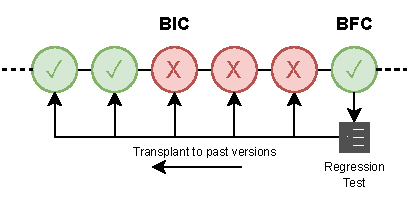
\includegraphics[width=0.8\textwidth]{pages/03-BugHunter/images/Model_Inverted.pdf}
  \vspace{-0.5cm}
  \caption{Simplified process leading to finding the first failing change (FFC), by running tests in past snapshots of the project.}
  \label{fig:process}
  \vspace{-0.5cm}
\end{figure}

The paper presenting the perfect test method~\cite{rodriguez2020bugs} states that one of the main limitations of the perfect test is that being able to construct a perfect test requires a deep knowledge of the bug, how it was fixed, and the project in which it was found. 
In our case, we assume that developers writing regression tests have all this knowledge, and therefore their tests will be close to the theoretical perfect test for the bugs they fix.


\subsection{The bugs dataset}
\label{subsec:dataset}

Defects4J~\cite{just2014defects4j} is a well-known dataset with 835 bugs from 17 Java open source software projects, including only bugs located in the source code, excluding those related to the build system, configuration files, documentation or tests. It has been used as ground truth in the evaluation of several implementations of SZZ-derived algorithms~\cite{neto2019revisiting,pokropinski2022szz,wen2019exploring,an2021reducing}. 
Previous studies have identified several issues that might threaten application of SZZ-derived algorithms: e.g., links to the repositories might have  changed~\cite{lawrence2001persistence}, repositories might have been deleted, moved, made private, or their history might have been altered~\cite{bird2009:promises_perils_git}.
However, Defects4J includes the whole source code management repositories of each project, avoiding the problems mentioned above.
All but one of the repositories in Defects4J are git repositories, which is the source code management we will target in our study.

% Defects4J is not only a dataset, but a whole framework for working with the repositories and bugs it includes. \as{This seems to contradict the first sentence of this section ``Defect4J is a well-known dataset...'' Please rephrase.}
% It provides a command-line tool for extracting information related to a bug (e.g., the fixing commit, the bug report, and the regression test), \as{This is odd: so far there has been no discussion that Defect4J contains fixing commits, this point will be made only in the next paragraph. Maybe move this paragraph further downwards?} get a copy of the corresponding repository, and other useful tasks, which makes it easy to work with the dataset. \as{The last fragment ``and other useful tasks...'' does not seem to be useful.}

Every bug included in Defects4J identifies the change (commit) fixing it (its BFC), and refers to a publicly available bug report which details the nature of the bug.
From here on we refer to changes as commits, since we will focus on git repositories.
% \as{It seems that we are using the words ``change'' and ``commit'' interchangeably. Moreover, we are also calling the same thing a ``node''. Can we maybe select one of the terms and use it consistently?}
% \michel{Now, from the second paragraph of Section~\ref{subsec:dataset} where the term commit is stated as the "change" defined above, only the term "commits" is used. The term "change" is kept in the Section~\ref{subsec:model} to be consistent with Gema's work.}
% \as{OK, we might like to add a sentence like ``From here on we refer to changes as commits'' or something similar.}
This bug report will be required when manually evaluating the detected BICs.
Therefore, the dataset complies with step (1) of the perfect test method. 
Associated with each bug there is also a regression test, included in the BFC, that exposes the bug. 
The dataset also provides its own commands to compile the code and execute the test in this commit. 
We will use this regression test as a perfect test for the bug, therefore complying with step (2) of the perfect test method.
Although the regression tests included in Defects4J have been reviewed by the authors of the dataset and emphasize in their tool that they have left out any flaky test, we have run each test 3 times in the BFC to verify that their results do not differ, and therefore we avoid including non-deterministic tests in the experiment.

The dataset does not include information about the commit that introduced the bug (if any), which we would need to verify that the result of step (3) of the perfect test method found the right change. 
However, the dataset provides a specific (synthetic) snapshot of the code without the fix (that is, with the bug present), in which we can check that the test fails. 
This supports our assumption that the regression tests identified in the Defects4J dataset can be used as perfect tests.

% \as{It seems that the previous paragraphs where describing the dataset as is, while the remaining part of the subsection discusses what we have done to it (excluding some parts). Would it be a good idea to split 3.2 into 3.2.1 and 3.2.2?}
% After examining the dataset, we found that the projects in it use different build systems, \as{At this point it is not clear why is it even important to know what build systems are used by the projects. Consider making this explicit.} among which we identified Maven, Gradle and Ant (all common Java build systems).\as{Is the comment ``all common Java build systems'' really necessary?}
%  In our case, we decided to build snapshots, and execute the transplanted tests, only with Maven or Ant. 
% Maven is one of the most widely used build systems in Java and offers the least problems when reproducing a build~\cite{sulir2016quantitative}. 
% Additionally, we also use Ant because many projects using Maven had used Ant at some moment in the past (Maven replaced Ant as the build system in many projects, including some in the dataset\as{Do we have a reference to support the claim that many projects moved from Ant to Maven?}). 
% Therefore, for transplanting tests to any commit in the past history of projects using Maven, in some of them we also need to support Ant. 
% Including Gradle didn't significantly increase our chances\as{I am not sure that the phrasing in terms of chances is precise; maybe rephrase?} of building snapshots and running tests, as only one of the projects selected uses Gradle, and this project also offers support for Ant, so it is included in our study.

From the whole Defects4J collection of projects, we excluded project Chart because it uses Subversion~\footnote{\url{https://subversion.apache.org/}} as version control system. 
We focus only on projects that use Git. 
As a result, we included in our experiment 16 projects out of the 17 found in Defects4J, with a total of 809 bugs of the initial 835 bugs.
Table~\ref{table:dataset-table} shows a brief description of the selected projects: the number of bugs it contains reported by the dataset, the number of stored commits, the dates for the first commit of the project and the last one (the last commit does not correspond to the last one in the official repository, since the projects in the dataset are stored as a copy of the git repository at a specific point in time). 
It should be noted that this dataset was extended in 2020, based on the original 2014 dataset~\cite{just2014defects4j}.

\begin{table}[]
    \caption{\label{table:dataset-table} Description of the projects used from Defects4J}
    \resizebox{\textwidth}{!}{%
        \begin{tabular}{|r|r|r|r|r|}
            \hline
            \textbf{Project} & \textbf{\# of bugs} & \textbf{\# of commits} & \textbf{First Commit} & \textbf{Last Commit} \\ \hline
            Cli              & 39                  & 914                    & 2002-06-10            & 2019-03-25           \\ \hline
            Closure          & 174                 & 2,898                   & 2009-11-03            & 2013-12-13           \\ \hline
            Codec            & 18                  & 1,795                   & 2003-04-25            & 2019-04-23           \\ \hline
            Collections      & 4                   & 3,091                   & 2001-04-14            & 2019-03-25           \\ \hline
            Compress         & 47                  & 2,682                   & 2003-11-23            & 2019-03-25           \\ \hline
            Csv              & 16                  & 1,290                   & 2005-12-17            & 2019-04-14           \\ \hline
            Gson             & 18                  & 1,476                   & 2008-09-01            & 2019-11-05           \\ \hline
            JacksonCore      & 26                  & 1,724                   & 2011-12-22            & 2019-04-24           \\ \hline
            JacksonDatabind  & 112                 & 5,241                   & 2011-12-22            & 2019-05-15           \\ \hline
            JacksonXml       & 6                   & 949                    & 2010-12-30            & 2019-05-05           \\ \hline
            Jsoup            & 93                  & 1,261                   & 2010-01-17            & 2019-07-04           \\ \hline
            JxPath           & 22                  & 598                    & 2001-08-23            & 2018-05-15           \\ \hline
            Lang             & 64                  & 3,596                   & 2002-07-19            & 2013-10-10           \\ \hline
            Math             & 106                 & 4,913                   & 2003-05-12            & 2013-10-16           \\ \hline
            Mockito          & 38                  & 3,262                   & 2007-11-15            & 2016-08-02           \\ \hline
            Time             & 26                  & 1,718                   & 2003-12-16            & 2013-12-04           \\ \hline
        \end{tabular}
    }
\end{table}

%Defects4J can be used to check if the operationalization of the perfect test method by using regression tests actually detects the commit that introduced each of the bugs. \as{It seems that the previous sentence is much more precise than the current phrasing of the RQ. Maybe rephrase the RQ?}
% For this, we check if step (3) of the method, which finds the FFC for the test, actually detects the BIC for the given bug.

\subsection{Transplanting the test to the past}
\label{subsec:transplant} 

Following the process shown in Figure~\ref{fig:process}, we have designed and implemented a Python tool that automates all the necessary tasks to transplant the regression test to the commits corresponding to past changes, and run it to determine if it fails or succeeds. 
For each bug in our subset of the dataset, it takes the following steps:

\begin{enumerate}
  \item \textbf{Extract information.} 
    By using the command-line tool provided by Defects4J, extract the fix commit, bug report and regression test for the bug.
  \item \textbf{Set up the repository.} 
    By using the Defects4J command-line tool, obtain a copy of the git repository of the project corresponding to the bug.
  \item \textbf{Execute the regression test on the fix commit.} 
    This will ensure that the test actually succeeds for this snapshot, which means that it succeeds when the bug is fixed (if not, the test would not check properly, as the perfect test method states). For this, the tool checkouts the snapshot corresponding to the bug fixing commit (BFC), and runs the regression test on it.
    In this step, the file containing the test is stored, in order to be transplanted into the previous snapshot (the test method, as well as the file name and the path where it is located is provided by the dataset).
  % \item \textbf{Execute the regression test in the commit prior to the fix.}
  %   This will ensure that the test actually fails in this snapshot, confirming that it detects the bug properly (if it succeeds, the test is not detecting the bug properly, in the sense defined by the perfect test method). 
  %   For this, checkout the snapshot corresponding to the previous commit, transplant the regression test, and try to run it.
  %   We refer to transplanting as placing the file containing the test (copied from the BFC) in the original path (recreating the original directory if necessary).
  \item \textbf{Execute regression test on all previous commits.}
    This will allow us to find the first failing change (FFC), which as we discussed, in the case of intrinsic bugs, will be the BIC that we are looking for. For this, the tool checkouts each of those past commits, transplants the test to each of them, and runs it in each of them. 
    The FFC will be the first one that fails after the last one that succeeds. 
    %The list of past commits is obtained through the command \textit{git log --reverse}, run from the BFC.
\end{enumerate}

In the steps that execute regression tests, the tool follows this procedure:
\begin{inparaenum}[\bf(1)]
\item \textit{checkout the corresponding commit},
\item \textit{transplant (copy) the regression test},
\item \textit{compile the source code},
\item \textit{compile the regression test}, and
\item \textit{execute the regression test}.
\end{inparaenum}
For compiling and executing we decided to use standard Maven and Ant commands, since the command provided by Defects4J only works with some specific commits (in the BFC and in a synthetic commit where the bug is present), and we needed to build and run the test on any of them (see previous discussion on finding the FFC at Section~\ref{subsec:model}). 
%However, we used the copy of external libraries provided with Defects4J, thus avoiding problems due to some of them no longer being available.

When the tool finishes all actions for a given bug, it reports the results of executing the regression test (if that was possible) for all commits prior to the BFC. These results include the success or failure of the different phases: building the source code, building the transplanted test code, running the regression test, and the result (fail or success) of running the test. 
In order to know the reasons for failures, the tool also keeps a log of the execution of each step.

In order to measure how far a test can be transplanted to the past and answering \textbf{RQ\textsubscript{3.1A}}, it is necessary to define a metric that allows us to measure how far we can transplant a regression test. 
We propose the \textit{Transplantability} metric. 
For a given bug for which we have a test that detects it, we consider all commits that are ancestors of the BFC, in chronological order, and from this ordering we will find a commit $n$ which is the oldest at which the test can be transplanted and executed. 
We define \textbf{Transplantability (in days)}, $T_{days}$ as the number of days between commit $n$ and the BFC. 
In the same way, we define \textbf{Transplantability (in commits)}, $T_{commmits}$ as the number of commits between 
%\as{What does ``between'' mean for a tree? Is there always a branch between $n$ and the BFC?}\michel{We consider the chronological order (as stated above), not the branches.} \as{Where did we say this? Do we want to somehow integrate this chronological idea in the definition of $T_{commmits}$? Is it not odd to somehow count commits belonging to completely different branches?}
%\michel{We rephrased the first part of the paragraph to explain that the commits are traversed in chronological order.}
commit $n$ and the BFC.
The two different ways of quantifying, together, are intended to give a more comprehensive view of how far we can transplant a test into past commits.

In Chapter~\ref{chapter:buildability} we had already stated that at least in the compilation of the source code we may face problems that will prevent us from continuing with the experiment. 
We also consider the likelihood that errors may also occur in the compilation of the regression test and in the execution of the test itself (i.e., that the test does not generate a report indicating whether the test passes or fails).

Problems related to compilability of source code, the compilability of the regression test code (the transplanted test), and the runnability of the regression test will be studied in order to answer \textbf{RQ\textsubscript{3.1B}}. 
To further understand these problems, we introduce three definitions: source code compilability, transplanted test compilability, and transplanted test runnability.

\textbf{Source code compilability} is defined as the percentage of snapshots in the past history of the BFC that could be successfully compiled.
This metric was originally defined by Tufano et al.~\cite{tufano2017there} and used in Chapters~\ref{chapter:buildability} and~\ref{chapter:testability}.
These previous studies took as reference commit the last one in the repository (the most recent one), considering as the commit history of the project all the commits previous to this one. 
In this chapter we will use as reference the BFC commit to define the commit history for each bug. In this way, we will calculate the Source code compilability of the commits previous to the BFC.

\textbf{Transplanted test compilability} is similar, but for the transplanted test: the percentage of snapshots in the past history of the BFC in which we could compile the transplanted test. 
These parameters let us know how often the reason for not being able of running the transplanted test was not being able to compile the test itself or compiling the source code in each of the snapshots.

\textbf{Transplanted test runnability} is defined as the percentage of snapshots in the past history of the BFC in which we could run (execute) the transplanted test without errors, producing a ``success'' or ``fail'' result, as stated in Chapter~\ref{chapter:testability}. The larger the test runnability, the more commits in which we could run the test. If it is 100\%, the perfect test method can be run for the whole history before the BFC. When test runnability is not 100\%, for some commits we cannot assess if the test fails or succeeds (because it doesn't run). Depending on success and fail in other commits, maybe we have to add the commit to the list of candidate BICs without being able of be more conclusive about it. Therefore, the transplanted test runnability shows how successful is the transplantation of regression tests to past commits.

\subsection{Identifying the Bug Introducing Change}
\label{subsec:identify-bic}

From the results obtained after transplanting the regression test on the commits prior to the BFC we can seek to locate the BIC.
At this point, we can revisit what ``all previous commits'' from Step 4 mean. 
In Figure~\ref{fig:process} we present the history of commits as linear. 
However, in a real git repository the commit history might not be linear: there are development models (as GitFlow~\footnote{\url{https://nvie.com/posts/a-successful-git-branching-model/}}) with git in which development is done in parallel branches, which are merged when convenient. 
Therefore, the history of a project can be considered as a directed graph. 
The previous theoretical model contemplated only a linear history of commits, which limits the understanding of this history. The consideration of the history as a graph to further refine the BIC search is a contribution of this work.
Each node represents a commit that will point to the commits that precede it (its parents), which can be one or more.

With this in mind, we developed Algorithm~\ref{alg:bic} to detect the BIC in this graph. 
This algorithm receives as parameters the graph, annotated with the result of running the tests (its status, which can be success, fail or error) and the identification of the BFC in that graph. 
%This algorithm returns the list of candidates to be the BIC. 
This algorithm traverses the graph using a depth-first search~\cite{cormen2022depthfirstsearch}, starting with an empty list of candidates, and trying to find the list of candidates to be the BIC, according to the perfect test method. 
For that, the algorithm finds the node $n$ in which the test fails and which preceding nodes succeed (success parents), which would make $n$ a candidate to be the BIC.

Since for some nodes we could not run the test (because it could not be compiled, it did not run, or the source code could not be compiled), we must consider that in these nodes the tests may or may not be executed successfully.
%Therefore, the algorithm finds all nodes in which the test fails, or cannot be run, and in all nodes preceding these nodes the test succeeds, or cannot be run. 
%All the nodes found by the algorithm would be the candidates to be the BIC.
\begin{footnotesize}
    \begin{algorithm}[t!]
        \caption{Algorithm to detect bug-inducing commits}\label{alg:bic}
        \SetKwInOut{Input}{Input}
        \SetKwInOut{Output}{Output}
        \SetKwInOut{Precondition}{Precondition~}
        \Input{A $\mbox{\sl graph}$ (commit history) and the $\mbox{\sl bfc}$}
        \Output{A list of candidates for BIC}
        \Precondition {The $bfc$ status (the output of the regression test) must be success
        % \as{I understand the intention but ``status'' does not seem to be defined. }
        % \michel{I clarify what ``status'' is at text}
        % \as{It might be a good idea to explain ``status'' here such that the algorithm becomes self-contained?}
        }

        $candidates \gets []$\;
        $queue \gets [bfc]$\;
        $visited \gets [bfc]$\;
        $temp\_candidates \gets []$\;
        
        \While{$ NotEmpty(queue) $}{
            $n \gets GetFirst(queue)$\;
            \If{hasFailStatus(n)}{
                $candidates \gets []$\;
            }
            $parents \gets GetParents(graph, n)$\;
            $successParents \gets True$\ \Comment*[r]{Control if all parents are success} 
            % \as{What does $successParents$ mean?}
            % \michel{I clarify at text}
            \If{$ isEmpty(parents) $\Comment*[r]{Reach first commit}}{
                    \eIf{size(queue) == 0}{
                        $break$\;
                    }{
                        $continue$\;
                    }
            }

            \For{$p \in parents$}{
                $successParents \gets successParents \And hasSuccessStatus(p)$\;
                \If{$ \neg hasSuccessStatus(p) $}{
                    \If{$ hasErrorStatus(p) $}{
                        $AddItem(candidates, n)$\;
                    }
                    \If{$ p \notin visited $}{
                        $AddItem(queue, p)$\;
                        $AddItem(visited, p)$\;
                    }
                }
            }
            \If{$ successParents \And \neg hasSuccessStatus(n) $}{
                \eIf(){$ hasFailStatus(n) $}{
                    \Return{$[n]$}\; 
                }{
                    $AddItem(candidates, n)$\;
                    
                    \eIf(){IsEmpty(queue)}{
                        \Return{$candidates$}\;
                    }{
                        $temp\_candidates \gets candidates$\;
                    }
                    
                }
            }
        }
        \Return{$temp\_candidates$} 
    \end{algorithm}
\end{footnotesize}

The algorithm operates under the following assumptions: (1) all the ancestors of the BIC are success commits, until the beginning of the history of the project, or until the features on which the test is built are introduced; (2) in the case of a commit with two or more parents, which generate branches, the BIC can only be in one of these branches.
The first assumption is based on the definition of the BIC: the first commit where the bug manifests, which following the perfect test method, means the first commit where the test fails. In other words, in snapshots previous to the BIC the bug is not present, and therefore the test, if it can be run, should succeed. The test may not run if it is designed on top of some feature (e.g., some function) that does not exist for some snapshot, because it was not yet implemented.
The second assumption is based on the unlikeness that the same bug (which is fixed by a single fix commit) is introduced in two different branches. 
% For any given bug, it may happen that the test does not succeed in the BFC. 
% This may happen because the source code or the test is not compilable, in which case we can say nothing: we just do not have enough evidence to guarantee that the test actually succeeds for the BFC, and therefore we do not run it (we considered this as a precondition for identifying the BIC). We will consider that we do not have enough data for this bug, and will ignore it in our study.

Our algorithm has as a precondition that the regression test can be run and gives a successful result in the BFC.
If this precondition is fulfilled, we can run the algorithm, and come with two different outcomes:

\begin{itemize}
\item \textbf{The test succeeds in some preceding commit.}
  We should find at least one parent commit of the BFC for which the test fails (we should have at least one snapshot where the bug is present). 
  Following the ancestors of those commit that fail, we eventually find one that succeeds. 
  If we find a commit $n$ where the test does not succeed, but it succeeds for all its parents, then $n$ should be considered the commit that introduced the bug. 
  In this case, the algorithm found a single candidate and returns it. If we find a commit $n$ where the test cannot be compiled, and it succeeds in all its parents, then all commits between $n$ and $m$, being $m$ the first descendant of $n$ where the test can be compiled and fails, are considered candidates. 
  In this case, we have found several candidates, and we cannot decide which one is exactly the BIC because we cannot run the test in them, but we know the BIC should be one of them.
\item \textbf{The test does not succeed in any precedent commit.}
  In this case, we should assume that the bug was always in the code, since the functionality tested by the test was introduced or that we cannot run the test for some reason (i.e., we are not able to compile the source code). In any case, we cannot find the BIC: either it doesn't exist, or it is hidden because we cannot run the test, so the algorithm returns an empty list of candidates.
\end{itemize}

As an example of how the algorithm works, Figure~\ref{fig:bug41} represents the commit history for Bug 41 of the JacksonDatabind project from Defects4J dataset. 
The figure includes only commits relevant to understanding how the algorithm finds the BIC, and consecutive commits (without forks or merges) of the same color have been reduced to one. 
Each commit is identified with a number, whose value simply indicates its chronological position with respect to the fix commit (BFC) in order to be able to refer to them.
Colors in the figure show if the regression test succeeds (green~\checkmark) or fails (red~$X$).

\begin{figure}[ht!]
  \centering   
  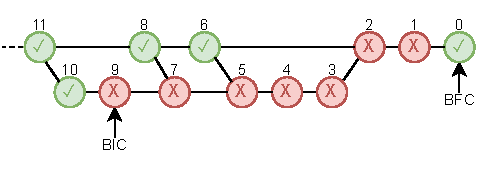
\includegraphics[width=\columnwidth]{pages/03-BugHunter/images/Databind_41_Inverted.pdf}
  \caption{Visual representation of the results of the experiment for Bug 41 of JacksonDatabind project.}
  \label{fig:bug41}
\end{figure}

In this figure we can see how Commit 2, although it has a green parent (Commit 6), cannot be considered as BIC, since it has another parent (Commit 3) where the bug is present. Following the ancestors chain, the algorithm will at some point find Commit 9, which is red, but for which all parents are green (in this case, only Commit 10). 
%All ancestors of Commit 10 are green too. 
Therefore, the candidate list in this case will include only Commit 9.

% As stated before, all the is fully automated in a tool implemented as a set of Python scripts (see Figure~\ref{fig:tool}). First, information about the bug (the BFC, the regression test that reveals the bug and the link to the test report) and the corresponding Git repository are extracted by \textit{ExtractBugsD4J.py} using the command-line tool provided by Defects4J (D4J). Then, the regression test is run on the BFC and all the commits preceding it, using \textit{RegTestExecutor.py}. The results of the building process for each commit, and the result of running the test is recorded. \textit{CommitGraph.py} uses these results to produce a labeled graph (with labels showing the results of building and test running), which is fed to \textit{Analysis.py}, which runs the Algorithm~\ref{alg:bic} to find BIC candidates.

% \begin{figure}[t!]
%     \centering   
%     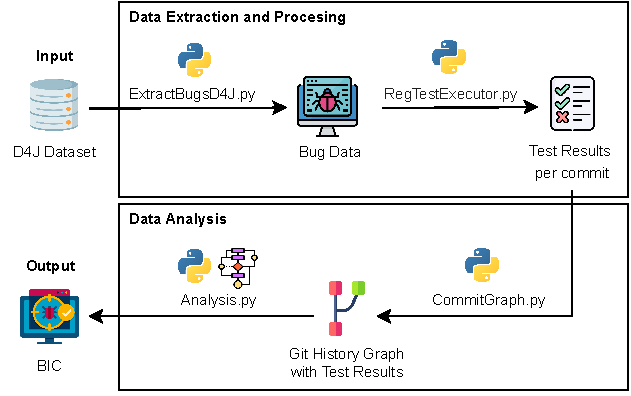
\includegraphics[width=\columnwidth]{images/RegressionTool.pdf}
%     \caption{Processes carried out by the tool. All scripts and documentation for the tool are available in the reproduction package (See `Reproducibility' section at the end of the paper).}
%     \label{fig:tool}
%     \vspace{-0.5cm}
% \end{figure}

%\as{This section seems to be too lengthy...}
%\michel{Huge refactor has been performed}

\subsection{Manual validation}
\label{subsec:manual}

To ensure that the results of our study can be considered as ground truth, we verified them by performing a manual validation of the BICs detected for each analyzed bug. For this purpose, we performed the following steps for each BIC detected:

\begin{itemize}
    \item Check and understand the bug report
    \item Check and understand the fixed functionality in the BFC.
    \item Check and understand the changed functionality in the candidate BIC
    \item Check the output of the test run
\end{itemize}

Following these steps, we categorized the BICs found in our study as true positives or false positives, using only true positives as the ground truth in order to generate a validated dataset of BICs.

%%% Local Variables:
%%% mode: latex
%%% TeX-master: "../paper"
%%% End:


\section{Experimental Results}
\label{sec:bug-hunter:results}
% jgb: Proposal for the text above
In this section we show the results of our study, answering the research questions presented in the introduction. 
The following results are intended to determine the extent to which we can operationalize the theoretical model proposed by \gema~
We have considered a total of 809 bugs in the Defects4J dataset, after filtering out bugs for the project we do not consider as explained in Section~\ref{subsec:dataset}. The results we found for each of those bugs are summarized in Figure~\ref{fig:experiment-overview}. 
This figure differentiates the cases in which, out of the total number of bugs, the regression test was found to pass again in some commit prior to the BFC from those that did not. In turn, from this first group, we differentiate the bugs from which we have been able to obtain a single candidate to be the BIC or several of them.
%\as{I guess that this figure should be somehow discussed?}
%\michel{I add a little explanation}

\begin{figure}[h!]
    \centering    
    % \begin{tikzpicture}[node distance=1cm,every node/.style={fill=white, font=\sffamily}, align=center]
%     % Specification of nodes (position, etc.)
%     \node (total)             [large]                                         { };
%     \node (buildable)         [large, below of=total]                         { };
%     \node (testBuildable)     [large, below of=buildable]                     { };
%     \node (success)           [large, below of=testBuildable]                 { };

%     \draw[-Latex]             (total) -- (buildable);
%     \draw[-Latex]             (buildable) -- (testBuildable);
%     \draw[-Latex]             (testBuildable) -- (success);

% \end{tikzpicture}
\begin{tikzpicture}[sibling distance=15em, level distance=2cm,
    every node/.style = {shape=rectangle, draw, align=center, top color=white,  }]
    \node {Total bugs \\ (809)}
      child { node {The regression test \\ succeeds in some precedent\\ commit(96)} 
          child { node {One candidate\\ found (67)} }
          child { node {Multiple candidates\\ found (29)} }
      }
      child { node {The regression test\\ does not succeed in\\  any precedent commit (713)} }
      ;
\end{tikzpicture}
  %  \vspace{-0.5cm}
    \caption{Summary of results for each of the bugs considered in the study.}
    \label{fig:experiment-overview}
\end{figure}

%%%%%%%%%%%%%
%    RQ1A    %
%%%%%%%%%%%%%

\subsection{How far can a test be transplanted into the past?}
\label{results:rq1a}

In Table~\ref{table:rq1a} we show the values for each of the interpretations of Transplantability for each bug. 
The values are aggregated by project, showing the mean and median for all bugs in each project. 
%The table also provides the aggregation of all bugs from all projects to obtain the mean and median Transplantability values for the dataset.
Additionally, we add in the table the relative position (\%) of commit $n$ (1) with respect to the total number of days elapsed between the BFC and the first commit of the project and (2) with respect to the total number of commits between the BFC and the first commit of the project. 
A value close to 0\% in this relative position indicates that we have barely been able to transplant the regression test, while values close to 100\% indicate that the test has been transplanted in most of the past (with respect to the BFC).

\begin{table*}[ht!]
    \caption{\label{table:rq1a} Transplantability (in days and in number of commits) for each bug, aggregated by mean ({\large $\mean{x}$}), 
    by median ({\large $\median{x}$}) and by the relative position of the oldest commit where the test could be transplanted ({$\%$}).}
    \resizebox{\textwidth}{!}{%
        \begin{tabular}{|r|r|rrr|rrr|}
            \hline
            \multicolumn{1}{|c|}{}                 &                  & \multicolumn{3}{c|}{$T_{days}$}                                                   & \multicolumn{3}{c|}{$T_{commmits}$}\\
            %\cline{3-8} \\
            \multicolumn{1}{|c|}{\textbf{Project}} & \textbf{\# bugs} & \multicolumn{1}{c|}{\textbf{\large{\large $\mean{x}$}}} & \multicolumn{1}{c|}{\textbf{\large{\large $\median{x}$}}} & \multicolumn{1}{c|}{\textbf{\%}} & \multicolumn{1}{c|}{\textbf{\large{\large $\mean{x}$}}} & \multicolumn{1}{c|}{\textbf{\large{\large $\median{x}$}}} & \multicolumn{1}{c|}{\textbf{\%}} \\ \hline
            \textbf{Cli}                            & 39                                     & \multicolumn{1}{r|}{910}  & \multicolumn{1}{r|}{1168} & 36.09                 & \multicolumn{1}{r|}{134}  & \multicolumn{1}{r|}{115}  & 34.67                 \\ \hline
            \textbf{Closure}                        & 174                                    & \multicolumn{1}{r|}{234}  & \multicolumn{1}{r|}{108}  & 36.63                 & \multicolumn{1}{r|}{451}  & \multicolumn{1}{r|}{187}  & 39.62                 \\ \hline
            \textbf{Codec}                          & 18                                     & \multicolumn{1}{r|}{703}  & \multicolumn{1}{r|}{427}  & 27.06                 & \multicolumn{1}{r|}{192}  & \multicolumn{1}{r|}{78}   & 26.12                 \\ \hline
            \textbf{Collections}                    & 4                                      & \multicolumn{1}{r|}{599}  & \multicolumn{1}{r|}{703}  & 11.05                 & \multicolumn{1}{r|}{178}  & \multicolumn{1}{r|}{213}  & 6.30                  \\ \hline
            \textbf{Compress}                       & 47                                     & \multicolumn{1}{r|}{1885} & \multicolumn{1}{r|}{2021} & 47.64                 & \multicolumn{1}{r|}{1223} & \multicolumn{1}{r|}{1326} & 82.18                 \\ \hline
            \textbf{Csv}                            & 16                                     & \multicolumn{1}{r|}{106}  & \multicolumn{1}{r|}{41}   & 3.11                  & \multicolumn{1}{r|}{41}   & \multicolumn{1}{r|}{27}   & 5.17                  \\ \hline
            \textbf{Gson}                           & 18                                     & \multicolumn{1}{r|}{1283} & \multicolumn{1}{r|}{1212} & 47.60                 & \multicolumn{1}{r|}{481}  & \multicolumn{1}{r|}{368}  & 41.70                 \\ \hline
            \textbf{JacksonCore}                    & 26                                     & \multicolumn{1}{r|}{444}  & \multicolumn{1}{r|}{450}  & 32.98                 & \multicolumn{1}{r|}{262}  & \multicolumn{1}{r|}{258}  & 34.00                 \\ \hline
            \textbf{JacksonDatabind}                & 112                                    & \multicolumn{1}{r|}{718}  & \multicolumn{1}{r|}{666}  & 43.92                 & \multicolumn{1}{r|}{1183} & \multicolumn{1}{r|}{1123} & 40.74                 \\ \hline
            \textbf{JacksonXml}                     & 6                                      & \multicolumn{1}{r|}{884}  & \multicolumn{1}{r|}{939}  & 40.49                 & \multicolumn{1}{r|}{256}  & \multicolumn{1}{r|}{239}  & 40.41                 \\ \hline
            \textbf{Jsoup}                          & 93                                     & \multicolumn{1}{r|}{437}  & \multicolumn{1}{r|}{240}  & 26.95                 & \multicolumn{1}{r|}{142}  & \multicolumn{1}{r|}{76}   & 18.33                 \\ \hline
            \textbf{JxPath}                         & 22                                     & \multicolumn{1}{r|}{607}  & \multicolumn{1}{r|}{532}  & 24.44                 & \multicolumn{1}{r|}{80}   & \multicolumn{1}{r|}{79}   & 21.65                 \\ \hline
            \textbf{Lang}                           & 64                                     & \multicolumn{1}{r|}{355}  & \multicolumn{1}{r|}{246}  & 14.88                 & \multicolumn{1}{r|}{283}  & \multicolumn{1}{r|}{206}  & 13.05                 \\ \hline
            \textbf{Math}                           & 106                                    & \multicolumn{1}{r|}{186}  & \multicolumn{1}{r|}{110}  & 7.60                  & \multicolumn{1}{r|}{280}  & \multicolumn{1}{r|}{178}  & 10.16                 \\ \hline
            \textbf{Mockito}                        & 38                                     & \multicolumn{1}{r|}{1664} & \multicolumn{1}{r|}{1552} & 96.61                 & \multicolumn{1}{r|}{1781} & \multicolumn{1}{r|}{1540} & 95.93                 \\ \hline
            \textbf{Time}                           & 26                                     & \multicolumn{1}{r|}{452}  & \multicolumn{1}{r|}{478}  & 28.02                 & \multicolumn{1}{r|}{97}   & \multicolumn{1}{r|}{77}   & 19.33                 \\ \hline
            \hline
            \textbf{All bugs}                       & 809                                    & \multicolumn{1}{r|}{585}  & \multicolumn{1}{r|}{302}  & 32.93                 & \multicolumn{1}{r|}{530}  & \multicolumn{1}{r|}{212}  & 33.83                 \\ \hline
        \end{tabular}
    }
\end{table*}


For a more comprehensive view of the Transplantability results, Table~\ref{table:rq1a-iqr} provides in detail the distribution of $T_{days}$ and $T_{commits}$ results.
First, we found that both metrics offer very similar results, showing that the average frequency with which a commit is added to these repositories is approximately 1 day. 
% \michel{Here I think a reviewer could tell us why we use two metrics that mean the same thing. Although it may seem intuitive, I have read other articles about the frequency of commits per day in open source projects and they are around 4 commits/day on average.}\as{I think that this was some of Gregorio's work? We need to comment on this.}
Regarding the minimum value for both metrics, we found the value 0, which indicates that for at least one project, it was not possible to transplant the test to the commit prior to the BFC. We found that for bug 79 of the Closure project the BFC includes a new function as part of the bug fix, being this function used in the regression test. Since this function does not exist in the previous commits to the BFC, the error obtained when transplanting the test to them is a failure in the compilation of the test code.

\begin{table*}[]
    \caption{\label{table:rq1a-iqr} Distribution of Transplantability results for all projects}
    \resizebox{\textwidth}{!} & \textbf{50\%} & \textbf{75\%} & \textbf{max} \\ \hline
      \textbf{$T_{days}$}    & 809              & 585           & 706          & 0            & 84            & 302           & 830           & 3,475         \\ \hline
      \textbf{$T_{commits}$} & 809              & 530           & 696          & 0            & 72            & 212           & 712           & 3,709         \\ \hline
      \end{tabular}
    }
\end{table*}

In order to evaluate the feasibility of our method, we check whether the BIC found by our tool falls within the $T_{commits}$ and $T_{days}$ for the different regression tests. In this case we can assume that, at least for the considered projects, the test can be transplanted far enough to allow the detection of the BIC. 
For the 67 BICs detected, we found that, on mean, they are 182 days  and 190 commits between the BIC and the BFC. 
The diversity of projects forces us to check, in addition, the median: 47 days and 49 commits respectively. 
According to the values of $T_{days}$ and $T_{commits}$ we can state that we have been able to transplant the regression tests far enough to be useful in detecting the BIC. 
%\as{This is an extremely bold statement. To claim usefulness we need to somehow hear this from the developers of the original projects but this is probably impossible since the data is likely to be old. Is there a way to say something about ``far enough'' without asking developers?}
%\michel{We rephrased the statement to focus on the ``feasibility'' of the method}

Nevertheless, there might be commits between $n$ and the BFC where the regression test cannot be compiled or run. This leads us to the next RQ.

\vspace{0.4cm}
\fbox{\begin{minipage}{0.9\textwidth}
    \textbf{\rqonea}
    For the dataset used, we have managed to transplant the regression test for a bug up to 585 days (530 commits) in the past on average. 
    For 50\% of the bugs, the regression test could be transplanted up to at least 302 days (212 commits).
    On average, regression tests can be transplanted to a 32.93\% of the days (33.83\% of the commits) between the BFC and the initial commit of the project.
\end{minipage}}

%%%%%%%%%%%%%
%    RQ1B    %
%%%%%%%%%%%%%

\subsection{How compilability and runnability problems impact the transplantation of the regression tests to the past?}
\label{results:rq1b}

In Table~\ref{table:results-per-project} we show average and mean data for the three metrics defined in Section~\ref{sec:bug-hunter:methodology}: source compilability, transplanted test compilability and transplanted test runnability.

\begin{table}[h!]
    \centering{\small
        \caption{\label{table:results-per-project} Source code compilability, transplanted test compilability, and transplanted test runnability for each bug, aggregated by mean ({\large $\mean{x}$}) and by median ({\large $\median{x}$}) per project. 
        Values are shown in percentages.}
        \begin{tabular}{|r|r|rr|rr|rr|}
            \hline
            \multicolumn{1}{|c|}{\multirow{2}{*}{\textbf{Project}}} & \multicolumn{1}{c|}{\multirow{2}{*}{\textbf{\# bugs}}} & \multicolumn{2}{c|}{\textbf{\begin{tabular}[c]{@{}c@{}}Source \\ Compilability\end{tabular}}} & \multicolumn{2}{c|}{\textbf{\begin{tabular}[c]{@{}c@{}}T.Test \\ Compilability\end{tabular}}} & \multicolumn{2}{c|}{\textbf{\begin{tabular}[c]{@{}c@{}}T.Test \\ Runnability\end{tabular}}} \\ %\cline{3-8} 
            \multicolumn{1}{|c|}{}                                  & \multicolumn{1}{c|}{}                                     & \multicolumn{1}{c|}{\textbf{\large{\large $\mean{x}$}}}     & \multicolumn{1}{c|}{\textbf{{\large $\median{x}$}}}    & \multicolumn{1}{c|}{\textbf{{\large $\mean{x}$}}}    & \multicolumn{1}{c|}{\textbf{{\large $\median{x}$}}}   & \multicolumn{1}{c|}{\textbf{{\large $\mean{x}$}}}   & \multicolumn{1}{c|}{\textbf{{\large $\median{x}$}}}   \\ \hline
            \textbf{Cli}                            & 39                                     & \multicolumn{1}{r|}{56.07} & 62.61                 & \multicolumn{1}{r|}{29.40} & 30.88                 & \multicolumn{1}{r|}{29.40} & 30.88                 \\ \hline
            \textbf{Closure}                        & 174                                    & \multicolumn{1}{r|}{59.24} & 54.36                 & \multicolumn{1}{r|}{33.52} & 17.63                 & \multicolumn{1}{r|}{33.52} & 17.63                 \\ \hline
            \textbf{Codec}                          & 18                                     & \multicolumn{1}{r|}{28.30} & 14.29                 & \multicolumn{1}{r|}{25.13} & 8.84                  & \multicolumn{1}{r|}{25.13} & 8.84                  \\ \hline
            \textbf{Collections}                    & 4                                      & \multicolumn{1}{r|}{97.94} & 98.98                 & \multicolumn{1}{r|}{5.73}  & 7.46                  & \multicolumn{1}{r|}{5.61}  & 7.37                  \\ \hline
            \textbf{Compress}                       & 47                                     & \multicolumn{1}{r|}{29.96} & 23.60                 & \multicolumn{1}{r|}{20.81} & 17.02                 & \multicolumn{1}{r|}{18.35} & 10.22                 \\ \hline
            \textbf{Csv}                            & 16                                     & \multicolumn{1}{r|}{19.07} & 17.38                 & \multicolumn{1}{r|}{5.26}  & 3.51                  & \multicolumn{1}{r|}{5.21}  & 3.51                  \\ \hline
            \textbf{Gson}                           & 18                                     & \multicolumn{1}{r|}{42.00} & 35.98                 & \multicolumn{1}{r|}{40.73} & 34.68                 & \multicolumn{1}{r|}{40.73} & 34.68                 \\ \hline
            \textbf{JacksonCore}                    & 26                                     & \multicolumn{1}{r|}{35.08} & 32.54                 & \multicolumn{1}{r|}{31.52} & 30.12                 & \multicolumn{1}{r|}{31.52} & 30.12                 \\ \hline
            \textbf{JacksonDatabind}                & 112                                    & \multicolumn{1}{r|}{88.37} & 90.17                 & \multicolumn{1}{r|}{13.77} & 14.22                 & \multicolumn{1}{r|}{13.77} & 14.22                 \\ \hline
            \textbf{JacksonXml}                     & 6                                      & \multicolumn{1}{r|}{89.65} & 88.81                 & \multicolumn{1}{r|}{24.49} & 24.59                 & \multicolumn{1}{r|}{24.49} & 24.59                 \\ \hline
            \textbf{Jsoup}                          & 93                                     & \multicolumn{1}{r|}{21.08} & 12.52                 & \multicolumn{1}{r|}{17.56} & 9.74                  & \multicolumn{1}{r|}{17.56} & 9.74                  \\ \hline
            \textbf{JxPath}                         & 22                                     & \multicolumn{1}{r|}{92.25} & 100.00                & \multicolumn{1}{r|}{21.93} & 23.57                 & \multicolumn{1}{r|}{21.93} & 23.57                 \\ \hline
            \textbf{Lang}                           & 64                                     & \multicolumn{1}{r|}{74.08} & 66.08                 & \multicolumn{1}{r|}{11.61} & 8.50                  & \multicolumn{1}{r|}{11.61} & 8.50                  \\ \hline
            \textbf{Math}                           & 106                                    & \multicolumn{1}{r|}{39.80} & 36.19                 & \multicolumn{1}{r|}{7.99}  & 5.86                  & \multicolumn{1}{r|}{7.99}  & 5.86                  \\ \hline
            \textbf{Mockito}                        & 38                                     & \multicolumn{1}{r|}{30.69} & 30.06                 & \multicolumn{1}{r|}{24.17} & 25.22                 & \multicolumn{1}{r|}{24.17} & 25.22                 \\ \hline
            \textbf{Time}                           & 26                                     & \multicolumn{1}{r|}{72.84} & 100.00                & \multicolumn{1}{r|}{20.72} & 6.47                  & \multicolumn{1}{r|}{18.89} & 4.12                  \\ \hline
            \hline
            \textbf{All}                            & 809                                    & \multicolumn{1}{r|}{53.43} & 49.89                 & \multicolumn{1}{r|}{20.92} & 12.36                 & \multicolumn{1}{r|}{20.71} & 12.00                 \\ \hline
        \end{tabular}
    }
    \vspace{-4mm}
\end{table}


Table~\ref{table:rq1b-iqr} provides in detail the distribution these metrics for a more comprehensive view of the results. 

\begin{table}[]
  \caption{\label{table:rq1b-iqr} Distribution of source compilability, transplanted test compilability and transplanted test runnability results for all projects}
  \resizebox{\textwidth}{!} & \textbf{50\%} & \textbf{75\%} & \textbf{max} \\ \hline
      \textbf{Src compilability}      & 809              & 53.43         & 32.26        & 0.26         & 24.88         & 49.89         & 84.45         & 100.0        \\ \hline
      \textbf{T.Test compilability}   & 809              & 20.92         & 23.93        & 0.10         & 4.26          & 12.36         & 26.67         & 100.0        \\ \hline
      \textbf{T.Test runnability}     & 809              & 20.71         & 23.98        & 0.10         & 4.12          & 12.00         & 26.58         & 100.0        \\ \hline
    \end{tabular}
  }
\end{table}

The reasons that prevent transplanting the regression test are directly related to these metrics and can be classified as follows:

\begin{itemize}
\item \textbf{Compilability of the source code} If the source code cannot be built for the snapshot, there is no way to build the regression test. 
Compilability of past snapshots has been studied in detail by Tufano et al.~\cite{tufano2017there},whose experiment in 2014 showed an average compilability of 100 Java projects of 37.74\%. 
As seen in Chapter~\ref{chapter:buildability}, we replicated this experiment in 2020 and a decrease in compilability was observed due to the lapse of time, 
%\as{Please be more explicit why the lapse of time could be expected to reduce the compilability value.} \michel{Below it is commented that one of the factors affecting compilability is the passage of time. I clarify it} 
obtaining a value of 25.09\%. The compilability may vary largely from project to project, and it will depend among other factors on the availability of third party modules needed to build the code, on the availability of the building tools in the right version, and on the complete automation of the building process. These factors are usually affected by time, and a degradation of compilability as time passes has been observed in these two previous studies.
In our case, the mean compilability of the snapshots previous of each bug is 53.43\% (with a median of 49.89\%). 
The value obtained is higher than that obtained in previous studies due to a combination of good practices by the authors of the Defects4J dataset; \patxi{Esto deberían ser dos puntos?}
% \as{do you mean that storing dependencies and adding configuration files are the good practices? Or are there some good practices (whatever they might be) and on top of them the developers store dependencies and adapt configuration files?}
% \michel{The configuration files and the storage of the libraries are the best practices that I want to emphasize. Further on I comment that it provides a high reproducibility of the experiments (understanding that these are good practices to follow for anyone who wants to make his dataset reproducible).} 
storing project dependencies and adapting their configuration files to ensure high reproducibility in the experiments (although only in the BFCs), together with additional adaptations made by the authors of this work, completing the adaptation of the configuration of each project to each commit of its history.
%\as{"relatively low" suggests comparison with some kind of baseline. How do our figures compare to those reported in the previous papers [36,22]?}
%\michel{Now is more clear and we have added the comparison with the previous studies + the reason why our results are higher + explain the modifications to improve the compilability.}
\item \textbf{Compilability of the regression test} If the test cannot be built, it cannot be run. The test is built on top of the snapshot, and it may not build because the code it expects in the snapshot is not present. This may happen because that code was still not implemented for a given snapshot. For example, this is the case if the test tests a certain function: in some past snapshot the function may not be implemented yet. This may also happen because the code was in the snapshot, but not in the way the test expects it. For example, this may happen in case of refactoring between the snapshot we are trying to build and the snapshot for which the test was designed. In general, these problems will be increasingly frequent for older commits with respect to the BFC, since more artifacts (code files, libraries or configuration files) could change since those snapshots to the one corresponding to the BFC, for which the regression test was designed. They will also be frequent in branches which for some reason lack some code needed by the test.
The aggregate results for the transplanted test compilability (20.92\% mean and 12.36\% median for all bugs) are strictly lower than source code compilability, since compiling the source code is a necessary step to be able to compile and run the tests. \patxi{This is different to the results from Chapther 4, where in general whenever the source code compiles, the tests compile as well. In this case, the fact that we are transplanting the test from the present to the past has an impact on its compilability.}
To the best of our knowledge, there is no large-scale study on the compilability of a test that is transplanted to past commits, so we do not have a baseline on which to compare the results obtained on this metric.
% \as{Can we find some kind of baseline to compare these numbers, similarly to the compilability figures for the source code?}
% \michel{There are no previous studies that transplant tests into the past and measure how far they can be taken. The closest is a study of ours (not yet published) in which we ran tests on all commits of a project.}
% \as{Can we comment that there is no publicly available baseline?}

\item \textbf{Runnability of the regression test} Even if the regression test can be built, maybe its run does not produce a result, but fails earlier due to some code not behaving as expected. 
% This may happen, for example, if the test calls some function that is expected to return a certain value, but returns some other because that was the case in the earlier version of the code corresponding to the snapshot. 
When aggregating all bugs together, the mean for transplanted test runnability is 20.71\%, and the median is 12\%. 
Which means that in half of the bugs the test could be transplanted successfully to less than 12\% of the commits (although the difference with the mean shows how in some bugs, the transplant was successful in a much higher fraction of the cases). 
These values are again slightly lower than the previous metric (the compilability of the regression test) since we need to compile the test code in order to be able to run it. In this case, the values are very close (or even equal) to those of the compilability of the regression tests, so we can affirm that if the transplanted test is successfully compiled, it can be executed.
Again, as far as we know, the runnability of a test transplanted to the past has not been addressed on a large scale.
Again, to the best of our knowledge, the runability of a test transplanted to the past has not been previously addressed.\patxi{La frase se repite dos veces?}
% \as{Also here, no other baselines?}
% \michel{Like the previous one, we have no previous study to compare ourselves with.}
% \as{As above?}
% In some projects, transplanting bugs to past commits usually works, with medians as high as 98.07\% in Gson, meaning that in this case for half the bugs tests could be transplanted to almost all commits. But in others, it rarely works, such as in Collections or Csv, where in half the bugs the test could be transplanted to less than 4\% of the commits.
\end{itemize}

We will discuss the problems of transplanting the tests in the past in more detail in Section~\ref{sec:transplant-discuss}.
% \michel{Initially, the (specific) problems why I could not transplant the test to the past belonged to the discussion. In this section we start from metrics (src/test compilability and runnability) and delve (not too much) into the reasons why they do not obtain higher values. In the specified section I describe in more detail which problems I found and how I solved them.}

When examining the numbers for each project, we can see how, even when it varies from project to project, transplanted test runnability is always very similar to transplanted test compilability, which means that if the test compiled, in general it runs. In other words: the main blocker for running a test is that the test does not compile. For compiling the test, we should compile the source code. Again, by looking at this table, we can see how in some cases, the blocker for compiling the transplanted test is that the snapshot does not compile (for example for Gson, in almost all commits for which the snapshot compiled, the test also compiled). But for most of them, even if the snapshot compiles, the test does not.

These results are relevant because they show that by improving the compilability of the source code, and of the regression test, we could improve transplanted test runnability, and therefore, the applicability of the perfect test method. They also show that some projects have a very low compilability. 
This may be due to age (See Table~\ref{table:dataset-table})
%\as{Maybe we need to describe each and every bug? In any case here we should refer to such a table/description...}
of those projects (maybe the developers of those projects were using old practices that do not interact well with modern tools), or to specific characteristics of those projects, that maybe could be fixed with more knowledge about their building configuration.

Despite all these factors, the fact that for some projects transplanted test runnability is high shows that at least in some cases the conditions to use the perfect test method with regression tests hold.

\vspace{0.4cm}
\fbox{\begin{minipage}{0.9\textwidth}
    \textbf{\rqoneb}
    The effectiveness of the transplant \patxi{transplantation?} is limited by compilability issues unrelated to the transplanted test (the snapshot does not compile 
    46.57\% of the time) or by compilability of the transplanted test (the test does not compile 79.08\% of the time, essentially because of the limitation in compiling the source code or because it relies on missing code). However, we found that when the test compiles, in general, the test can be run. Therefore, compilability of the source code is a blocker that, when improved, could improve the transplanted test runnability.
\end{minipage}}

%%%%%%%%%%%%%
%    RQ2    %
%%%%%%%%%%%%%

\subsection{Can the BIC for a given bug be found using its regression test?}
\label{sec:rq2}

Following on with the chart in Figure~\ref{fig:experiment-overview}, to answer $RQ_{3.2}$ we will study in which cases the test succeeded in some precedent commit, and in those cases, how many candidate BICs were found. We consider the following scenarios as defined in our methodology. 

\textbf{The test does not succeed in any previous commit.}

From the total 809 bugs, in 713 the regression test did not succeed in any commit previous to it. 
In these cases, the perfect test method (using regression test as perfect tests) does not allow us to identify candidates for being the BIC. 
Since the test never succeeds in commits previous to the BFC, we cannot find the commit in which the bug was introduced. 
In the snapshots corresponding to some of those commits this is because the test cannot be run (and therefore we don't know if the bug is present or not in them), and in some others because it can be run, but fails (and then we know that the bug is present).

The reasons for the test not running (the test was not successfully transplanted) were already explored in the previous section, and in many cases are related to compilability problems. 
The fact that the tests are executed (successfully transplanted) but fail in all commits prior to the BFC is a case contemplated and addressed by the perfect testing \patxi{test} method: it means that the bug is present in those snapshots since the feature tested was introduced.
However, if we cannot find a previous commit for which the test succeeds, we have no evidence of where the BIC is.

\textbf{The test succeeds again in some past commit.}

For the remaining 96 bugs, the test succeeds in at least one commit previous to the BFC, and therefore we can provide more conclusive results by running the perfect test method.

For 67 bugs out of these 96, our algorithm produces a single candidate to be the BIC. 
The regression test succeeds in snapshots previous to this BIC candidate, which means it is the FFC (First-Failing Change), and following the perfect test method, the commit that introduce the bug (BIC). 
In 8 of these cases, the BIC was found in a direct parent of the BFC, which means the bug was detected and fixed very quickly after it was introduced. 
This is due to a practice known as \textit{Backtracking}~\cite{yoon2012exploratory,yoon2014longitudinal}, where the developer reverts part or all of the change \patxi{changes?} made when an issue is reported.

For the 29 remaining bugs, the algorithm finds multiple candidates. 
If $n$ is the first commit (going backwards from the BFC) in which the test succeeds, we have several candidates if for one or more commits that are right before $n$ (again, going backwards from the BFC) the test could not be executed (we are not able to compile the code or the test).
In those cases, since the test could not be run, we do not know if the bug is present or not, and, according to the definition provided by~\gema, any of them could be the FFC (the first failing change).
So, all of them, including the last one that failed (again, in the same order), are candidates to be the BIC. 
Without more information, we cannot assess which one of them is really the BIC.

%\as{Is it possible that none of them is the BIC? If yes, ``which'' in the previous sentence might be a wrong word choice.}
%\michel{Given that there is a commit in the past where the test passes again (but in the commits following this one the test cannot be executed) and having verified that when the test can be executed, it locates the commit that introduced the error, we assume that indeed one of the candidates is the BIC. The Gem model does not contemplate that there is no BIC when we find a test that happens again in the past.}
%\as{Do we want to make this assumption explicit?}
%\michel{We rephrase stated that we follow the definition provided by Gema}

\vspace{0.4cm}
\fbox{\begin{minipage}{0.9\textwidth}
    \textbf{\rqtwo}
    Yes, at least for those cases where a functionality no longer behaves as the regression test expects it. 
    The regression test can be transplanted to past commits, and using the perfect test method with the regression test as perfect test, the BIC can be found. 
    In our case, for the 809 bugs for which we could assess the regression test detected the bug, we could use the method to identify precisely the BIC in 67 bugs, and to provide a list of candidates for other 29 bugs. 
    The bugs for which the method did not work were mainly due to not being able of running the test, because of compilability or runnability problems, in addition to the contemplated case in which the tested feature has always contained the bug.
    In general, when regression tests could be run, the method worked.
\end{minipage}}

\subsection{Validation of results}

%\as{We seem to assume that BIC is (at least theoretically) unique but what if the bug is introduced through interplay between several commits?}
%\michel{As I understand Gema's model and how regression tests work, the first commit in which the test fails and its parent (or parents) have a success score on the same test should be the BIC. If there have been changes in different commits, our method will detect the first change that actually breaks the functionality as it is expected to work in the regression test.}
Once we have detected the BIC for 67 bugs through the perfect test method, we want to ensure that the BIC found is actually the BIC, the commit that introduced that bug. Following the steps already described in Section~\ref{sec:bug-hunter:methodology}, we checked manually all these cases, finding that all of them are true positives. This result allows for two conclusions:
\begin{itemize}
\item The perfect test method can be used to identify the bug introducing change, with regression tests as perfect tests, at least for those cases where a functionality no longer behaves as the regression test expects it.
\item We have a ground truth dataset of 67 bugs for which we know the BFC and the BIC, which can be used to evaluate methods for finding the BIC.
\end{itemize}

This manual analysis also allowed us to explore in some detail how those commits introduced the bug. We found the following two cases:
% \reviewer{This doesn't seem very insightful. One could consider that all commits are either bug fixes, refactorings or introducing new features. You find two out of three. Maybe it is surprising that you don't find new features that introduce bugs.  But the dataset is also pretty small.}
% \michel{If we consider a new feature such as, for example, adding additional cases within a function, then we have found it (See \url{https://github.com/FasterXML/jackson-databind/commit/a6443b2467542314065ce4545bfb52d5df2a76ed}). If the reviewer is referring to a new feature, such as a new module or class that would cause existing functionality to fail, we have found no cases.}

\begin{inparaenum}[\bf(1)]
\item \textbf{The bug is introduced in a commit marked as FIX}. 
This means that the commit was trying to fix another bug, but while doing that, it introduced a new one. For example, Bug 24 of the JacksonDatabind project has a BIC which is the BFC of another bug. 
The bug fixed in that BIC deals with date serialization, changing several classes for that. 
One of those commits, which is reverted in the BFC for Bug 24, was the one introducing that new bug.
Previous studies~\cite{guo2010characterizing,purushothaman2005toward,yin2011fixes} also state that bug-fixing commits are more likely to introduce a new bug in the software.
%\as{There is some research on fixes that introduce bugs, we need to cite it.}
%\michel{I have added some relevant citations. If you know of any more, do not hesitate to complete it.}

\item \textbf{The bug is introduced as a refactoring or reimplementation}. 
This case will be illustrated with Bug 23 of the Jsoup project (an HTML parser).
The bug is that the special entities that include numbers, to display fractions in HTML do not recognize the numbers, so they do not work as expected  (i.e., the string ``\&frac12'' should generate ``½'').
In the commit marked as BIC by our tool, there is a refactoring of the parse functionality, the main method of the library. 
This function goes from internally using the Parser class to using TreeBuilder (a new class). 
This refactoring brings with it the creation of new classes (that TreeBuilder needs to operate), among which we will highlight Tokeniser and CharacterReader.
In the BFC the method consumeLetterThenDigitSequence is added to the CharacterReader class, while in the Tokeniser class the call to consumeLetterSequence is changed by another one to the method consumeLetterThenDigitSequence (from CharacterReader) and solving the bug by considering numbers as part of an entity.\patxi{Esto es duro de leer y entender, quizá un diagrama UML con el refactoring podría ayudar}

% For example, Bug 23 of the Jsoup project, has a BIC in which the commit message states that it is the refactoring of a functionality in which several classes are affected. 
% In the BFC for this bug, only one function is fixed, which is the one that makes the test pass again. 
% In fact, this bug was present in the code for 86 commits. 
% \as{Sorry, I do not understand what has happened here. Did the BIC perform refactoring incorrectly, inadvertently introducing a bug; or was BIC a correct refactoring and it preserved earlier behavior subsequently preserving an earlier bug as well?}
% \michel{The BIC is a refactoring of several classes. In one of them a regression was introduced by the developer}
% \as{Maybe state explicitly that a regression was introduced in one of the classes affected.}
\end{inparaenum}

%\jgb{This text below could be moved to the discussion, but I think that a least a short introduction should be here, because of the importance of this result.}

This manual validation shows one of the most important results of our study: a collection of bugs with an identification of the BIC that introduced them can be produced automatically from a collection of BFCs using the perfect test method, with regression tests as perfect tests. 
These collections could be used to produce ground truth datasets for evaluation analysis, as we do in this study, but also for any other study where a collection of BICs is needed, such as those on how bugs are introduced.
In this chapter we provide~\datasetName~as one of these collections obtained from the Defects4J bug dataset, with a total of 67 identified BICs.

%%% Local Variables:
%%% mode: latex
%%% TeX-master: "../../../Tesis.tex"
%%% End:


\section{Discussion}
\label{sec:bug-hunter:discussion}
% After presenting the main results, and its analysis, in this section we discuss the details of our research: the difficulties of running a present test in the past, the limitations of SZZ implementations, a post-study where we compare the generated dataset with a pre-existing one, the implications of our study for a developer and the threats to validity.

In this section we will discuss in detail the difficulties of transplanting a test into the past~\ref{sec:transplant-discuss} and the implications of our work for practitioners~\ref{sec:implications-practitioners} and researchers~\ref{sec:implications-practitioners}.
We will also discuss the contribution of the generated dataset through 
\begin{inparaenum}[\bf(1)]
    \item an evaluation of SZZ-based tools on it~\ref{subsec:szz-tools} and
    \item a comparison of our dataset (\datasetName) with a previous BICs dataset using Defects4J as bug dataset~\ref{sec:induce-benchmark}.
\end{inparaenum}
Finally, we discuss the threats to validity of this chapter (Section~\ref{sec:threats}).


\subsection{Transplanting tests to the past}
\label{sec:transplant-discuss}
%\as{The purpose of this section is not clear.}
%\michel{I have rewritten part of the section, giving it more context and purpose, as well as eliminating the abuse of bullet points.}
% \michel{My idea here is to raise the difficulties encountered in running the tests in the past}

% \grex{We should point out that we depend on regression tests. How many projects do have such tests? Is the trend that more and more projects are having them?}

% \michel{I am afraid we do not have an in-depth analysis of how many of these tests there are. It is true that most of the tests we use as "perfect tests" are included in the BFC commit and in other projects we have detected this dynamic of fixing a bug and adding the test that checks if the bug is present or not.}


% The tool proposed in this work is based on the idea of using the test that detects the bug in the fix commit in past commits. 
% To do so, the tool copies the file of this test in order to run it on every commit in the past. 
% Each of the steps involved in this process are susceptible to failure for different reasons and during the development of the tool they have had to be mitigated. 
% These limitations imply a research challenge by limiting the effectiveness of the proposed tool.

% The first limitation we face is \textbf{building past source code}.
% Being able to build the source code of a commit is an essential step to be able to run the tests.
% Previous works on buildability in past commits~\cite{tufano2017there, maes2022revisiting} shows that a considerable part of a project's commits (in its master or main branch) are not compilable. 
% One of the main reasons why a commit is not compilable is usually because of a dependency resolution problem. 
% The main mitigation applied has been to use, as much as possible, the libraries and build files prepared by the creators of Dataset4J. 
% Although useful, these resources were prepared for specific commits and had to be generalized for any commit. 
% This measure has considerably increased the buildability of most projects.

% Even if you compile the source code, we may encounter problems when \textbf{building past tests}.
% Although we only run the test that reveals the bug, in Java we need to compile all test files prior to execution. 
% This means that if there is a problem compiling one of these tests, even if it is not used, it makes it impossible to continue with the experiment.
% A possible mitigation measure could be to delete all these tests, considering that there could be a dependency between these test classes and the one we want to test (e.g., inheritance of a parent class).

% Transplant a code file from the test to previous versions (\textbf{building regression test in past commits}) is not a simple task. 
% Assuming the test can be placed in the same directory, it is necessary to be able to properly test the functionality. 
% If it has changed over time (e.g., a function whose parameters have changed) the test may not compile, and therefore we may no longer be able to run it in the past.

% Finally, when we \textbf{run the regression test in past commits}, the result may not be as expected. 
% We have encountered cases where it seems that it is not only necessary to carry the test code into the past, but that the test itself has artifact dependencies that must be carried over along with the test code itself. 
% This limits the ability to fully automate the process, as a manual analysis of the possible dependencies that the test may have is necessary.
% These cases require a semi-automatic setup so that any artefacts required by the test can also be copied to past commits to ensure that the test can run.

% The mentioned problems and mitigations have been considered when building the tool proposed in this work.

% It is worth mentioning that the projects that make up the Defects4J dataset are Java libraries, not end-applications for a non-developer user. 
% The regression tests used are unit tests that are usually agnostic to the execution environment. 
% However, some of these tests have proven to be flaky, as mentioned in Section~\ref{sec:rq1}. 
% These tests may not even pass the fix commit, so they are not able to detect the change that introduced the bug. 
% In any case, they represent a non-significant sample within the set of tests used in the experiment.

% \patxi{We should also mention, here or anywhere else we find appropriate, that these tests are usually unit tests. Maybe by describing in more detail the Defects4J dataset, composed mainly of java libraries that do not usually have integration or e2e tests. This is also important to emphasize that when the test doesn't pass it is rare that the cause is flakiness (although some rare exceptions occur, like runtime-assertion found). Indeed, as we did a manual check of all of them, we can just say that we identified the flaky tests.}

% jgb: Proposal for substituting the text above
One of the main reasons for proposing the operationalization of the perfect test method using regression tests is that these (regression tests) are present in many modern projects. This means that the technique could be used in many of them, if those tests can be transplanted successfully to past commits. However, in Section~\ref{results:rq1b} we showed how in many cases this was not possible, and how much success we had in the different phases of the process (compilation of the snapshot, compilation of the test, and execution of the test). These problems clearly limit the effectiveness of the technique.
In fact, in Chapter~\ref{chapter:buildability} (and in previous studies~\cite{tufano2017there}) we notice that it is relatively usual that a considerable fraction of past commits in a project are not automatically compilable as such. 
However, we have also discussed that some reasons for those problems (such as the availability of dependencies or the suitability of build configurations) can be mitigated. 
To mitigate these problems, our tool allows to include a script in which the user can define fixes to be applied to each commit in which the regression test is executed. 
The authors of the Defects4J dataset follow a similar approach (from which we draw our inspiration). 
They provide manually generated configuration files so that the tests can be run on the BFC and on a synthetic version of the BFC without the fix code (with the aim of providing a commit where the bug is revealed).
These configuration files resolve some dependency issues by providing these dependencies as part of the Defects4J framework.
For 488 bugs out of 809, we have taken advantage of these configuration files, making some modifications to them, in order to transplant them together with the regression test and ensure high compilability of past commits.
The resolution of dependencies from external repositories is one of the main causes of failure in the build of Java projects~\cite{tufano2017there}.
One of the main advantages offered by these configuration files is that the project dependencies are obtained as local files (which are part of Defects4J) instead of downloading them from a remote repository, solving the above-mentioned problem.
%\as{The word ``some'' makes the entire discussion vague. How often did we benefit from these configuration files? Can we recommend potential users of the tool to always use these files? If not, when yes and when no?}
%\michel{The numbers are now displayed. Using these configuration files is somewhat limited to this experiment, in projects outside the dataset. The developer should ensure that the configuration files for each commit can be built, or the researcher should create his own "transplantable" configuration file.}

In the following we discuss other relevant modifications and fixes included, based on the suggestions proposed in Section~\ref{sec:buildability:discussion}.
We find references to dependencies (not included in Defects4J) that include the suffix ``-SNAPSHOT'', which indicates that this is a volatile development version and is sometimes removed from the dependency repositories (causing the impossibility to compile a project that depends on them). 
For 15 bugs we found that this dependency was included in the BFC, and the compilation of the BFC failed due to it, thus preventing our method from being able to work (the compilation and test execution at the BFC, with a success result, is a precondition for our method). 
The removal of this suffix, forcing it to use the stable version of that dependency, has allowed us to compile the BFC of these 15 bugs, allowing our method to start finding the BIC for them.
In 131 bugs from 6 projects we faced problems with source code parsing (due to the inclusion of unrecognized characters in strings or comments). 
Two different types of fixes have been used to solve this problem: 
\begin{inparaenum}[\bf(1)]
    \item modify the encoding at configuration file that is transplanted to the past along with the regression test or
    \item modify the snapshot configuration file to include the new encoding.
\end{inparaenum} 
We have also had to consider, in one project (Joda Time), that the code directories may change location (be placed in subfolders) in older commits, so it has been necessary to automate their re-structuring so that it can be compiled.

Building transplanted tests was also a problem. First, the standard way of building tests in Java requires building all of them together. 
This means that if there is a problem compiling just a single test, even if we do not have the intention to run it, because we only want to run the transplanted test, we cannot run it. 
This effect could be mitigated by ensuring that only the transplanted test is compiled, with the risk, maybe, of having dependencies on some test classes that are not run (e.g., inheritance of a parent class). Fortunately, we also observed that once the test was compiled, it almost always runs successfully.
In any case, for 14 bugs, we have automatically removed in the past commits some problematic tests (that did not compile) and were not related to the regression test.
For 10 bugs, it has been necessary not only to take the regression test to past commits, but also to take a file on which the test depends (auxiliary classes created specifically for that test).

\subsection{Implications for practitioners}
\label{sec:implications-practitioners}

When developers receive a bug report, in some cases along with the description there is a test that reveals the bug. 
This practice is common in open source projects, such as those of the Apache Foundation~\cite{iida2016improving}.
In some others, developers start by building that test before trying to fix the bug. In both cases, these regression tests are available before starting to fix the bug. The operationalization of the perfect test method with these tests allows to automatically find the BIC for that bug, assuming that the project took care of facilitating transplanting tests to the past (something that they can do by maintaining some rules on how to compile the source code as the project evolves). 
Therefore, when starting the process to fix the bug, the developer would have a hint about how the bug was introduced, which may be invaluable for speeding up the fixing process.

\subsection{Implications for researchers}
\label{sec:implications-researchers}

We have found an automatic method for producing a reliable collection of BICs, given their BFCs and their regression tests. 
This may be quite important for producing much larger datasets with BFC and their BICs, which could be used by researchers not only to evaluate algorithms for finding BICs, but also for other research purposes, such as training models of analyzing how bugs are introduced. Maybe those datasets could be biased, because they would only include bugs for which our method worked. But by improving compilability of past commits and transplanted tests, we think that the bias can be severely reduced, at least for some projects.

\subsection{Evaluation of SZZ derivatives}
\label{subsec:szz-tools}

Thanks to our subset of the Defects4J dataset with 67 bugs with verified BICs, we can evaluate the performance of the implementations of SZZ derivatives. 
We will use this dataset as the ground truth, and will run the implementations to check to which extent they correctly identify the right BIC for each bug.
We will analyze in detail those bugs where the implementations of SZZ derivatives are not able to find the BIC.

Several implementations of the SZZ algorithm and derivatives of it have been presented in the literature. However, for many of them their implementation has not been published, which has made it difficult to reproduce their results~\cite{rodriguez2018reproducibility}. 
Fortunately, several recent studies~\cite{borg2019szz,lenarduzzi2020openszz,pokropinski2022szz,rosa2021evaluating} provide public implementations of their algorithms. 
We evaluate their performance in finding the BIC, considering the manually validated results of our study as the ground truth.

% \as{Why have we chosen these seven implementations rather than some others?}
% \michel{These are all the available implementations of SZZ. Gema points out in a paper (which we have cited) that despite the several publications in the area, the implementations were rarely shared.}
% \as{I have rephrased the following sentence, please check.}
At the moment of writing there are seven publicly available implementations of SZZ variants:
%In this evaluation study we have considered the following seven variants of SZZ: 
%Rosa et al. recently implemented several SZZ variants in PySZZ, while making a comparison between them~\cite{rosa2021evaluating}. 
%The implementations compared in this study are as follows:
\begin{itemize}
    \item OpenSZZ~\cite{lenarduzzi2020openszz}. It is based on the original version of the SZZ~\cite{sliwerski2005changes}.
    \item PySZZ~\cite{rosa2021evaluating}. Includes five implementations of SZZ-derived algorithms: ag, l, r, ma and ra.
    SZZ-ag was proposed by Kim et al.~\cite{kim2006automatic} and is based on the original SZZ algorithm~\cite{sliwerski2005changes}, solving some limitations related to cosmetic changes in the code, such as moving a bracket to another line.
    SZZ-l and SZZ-r were proposed by Davies et al.~\cite{davies2014comparing} and is based on SZZ-ag, using two different criteria to select the BIC among the candidates: SZZ-l uses the largest candidate (the commit with the highest number of changes), while SZZ-r uses the most recent candidate.
    SZZ-ma was proposed by Costa et al.~\cite{da2016framework} and is based on SZZ-ag, excluding from the BIC candidates all commits that do not include changes to the source code, including merges between branches.
    SZZ-ra was proposed by Neto et al.~\cite{neto2018impact} and is based on SZZ-ma, excluding from the BIC candidates those commits that include refactoring operations.
    \item SZZ Unleashed~\cite{borg2019szz}. This variant partially implements an algorithm proposed by Williams and Spacco~\cite{williams2008szz} based on SZZ-ag, improving it by using a line-number mapping approach~\cite{williams2008branching} and DiffJ~\footnote{\url{https://github.com/jpace/diffj}} (a java syntax-aware diff tool). We emphasize that it only partially implements it since it does not use DiffJ.
\end{itemize}


For our work, we have selected these seven implementations of the SZZ to examine their results on the BICs detected by our tool. 
These implementations will identify, for each bug, a list of commits that are candidates to be the BIC, starting from the BFC for that bug. For evaluating each implementation, we have computed the number of commits that they included in the list of candidates for each bug, and the number of bugs for which the correct BIC is in the list of candidates. 
We have then aggregated the numbers for each implementation, computing the total number of bugs for which it correctly included the BIC within the list of candidates, its percentage over the total number of bugs (67), or \emph{hit rate}, and the average number of BIC candidates per bug (including those bugs for which the implementation produced zero candidates). These results are shown in Table~\ref{table:szz-results}.
%\as{Do different implementations make the same mistakes or different ones?}
%\as{Would it be a good idea to use some kind of ensemble predictor that combines all seven SZZ variants? }
%\michel{Since we have moved this section to the discussion, perhaps this can be left for another paper.}
\begin{table}[h!]
    \caption{\label{table:szz-results}Results of SZZ algorithms on our BIC dataset}
    \resizebox{\textwidth}{!}{%
        \begin{tabular}{|l|r|r|r|}
        \hline
        \textbf{SZZ Implementation} & \textbf{Correct BICs} & \textbf{Hit rate} & \textbf{Candidates (avg)} \\
                            \hline
                            OPENSZZ        & 14 & 20.90 & 0.97  \\ \hline
                            SZZ UNLEASHED & 4  & 5.97  & 14.30 \\ \hline
                            PYSZZ-ag      & 34 & 50.75 & 1.30  \\ \hline
                            PYSZZ-l       & 11 & 16.42 & 0.63  \\ \hline
                            PYSZZ-r       & 17 & 25.37 & 0.63  \\ \hline
                            PYSZZ-ma      & 42 & 62.69 & 2.07  \\ \hline
                            PYSZZ-ra      & 32 & 47.76 & 1.36  \\ \hline
        \end{tabular}
    }
    \vspace{-4mm}
\end{table}

% The results show a great variability of the algorithms in their ability to identify the BIC.
% Moreover, even the combination of all algorithms fails to identify BIC for 13 bugs out of the 49. 
% These bugs 
% %(which will be analyzed in detail in Subsection~\ref{subsec:szz-limitations}) 
% have in common that the BFC does not correct the same lines that were introduced in the BIC, so the premise of the SZZ fails, and the SZZ algorithms cannot find the BIC. 
% This evidences a known limitation of SZZ-based approaches. Our tool contributes to the state of the art to correctly identify BICs for this kind of bugs.\as{Can we compare $\frac{13}{49}$ with other studies of limitations of SZZ? Is the SZZ assumption is more/less often violated in our dataset than in the previous studies?}

% jgb: Below, my proposal for the text above
The results show a great variability in the ability of the implementations we have evaluated to identify the correct BIC, for the bugs in~\datasetName. It is remarkable that the hit rate is relatively low, except for the most advanced implementations of PySZZ (ag, ma and ra), which obtain an acceptable hit rate despite not having the information on whether the bug is present or not that the perfect test method provides.

There is also great variability in the number of BIC candidates produced per bug, from 0.63 to 14.30. 
However, for most implementations (all of them but one) the number of candidates per bug is relatively low (less than 2, in average). 
This means that they are reasonably precise, given that they only use limited information.

In addition, for 19 bugs none of the SZZ implementations included the right BIC in the list of candidates. 
% These 13 bugs are detailed below:
% \begin{itemize}
%     \item \textbf{Compress Bug\_45} 
%     In the BIC of this bug, a condition is added to the source code that causes a test to fail. 
%     This is fixed without removing the check, but by extending the source code. 
%     The lines changed in the BFC are not the same as in the BIC, but they are from the same file.
%     \item \textbf{JacksonCore Bug\_11} 
%     The commit prior to the BIC was a commented-out call to a function. 
%     In the BIC this call is implemented. 
%     In the BFC it is checked that this function should be called with another function for specific cases.
%     \item \textbf{JacksonCore Bug\_10}
%     In the commit prior to the BIC there was a branch of the code which, if reached, would raise an exception warning that a feature was not available. 
%     In the BIC this is replaced by the actual implementation, which introduces the error. 
%     In the BFC a validation is added as to whether it is really necessary to execute that code, but the same lines of code are not touched.\as{So the BFC is not really a fix?}
%     \item \textbf{JacksonDatabind Bug\_35}
%     The BIC is a FIX that changes a deserializer. 
%     The BFC changes another deserializer (different, more generic and may use the previous one) to pass the test.
%     The changes to the source code are not even in the same file.
%     \item \textbf{JacksonDatabind Bug\_59}
%     A function was refactored on BIC (and the bug was introduced). 
%     This method is fixed on BFC adding a new line that edit the return variable (but not the same lines\as{again, please be more explicit.}).
%     \item \textbf{JacksonDatabind Bug\_72}
%     The class "A" is used instead of "B" \as{Why would one not use the real names?} in the BIC. 
%     The change of class introduces an error as some of its methods are not overridden. 
%     To make the test pass in the case of an error, these methods are re-implemented in a class C that inherits from A.
%     \item \textbf{Jsoup Bug\_43}
%     In the BFC the equals method is changed to compare directly with ==. 
%     In the BIC the equals method, which used to work as a == is changed to be more specific and that causes a bug.
%     \item \textbf{Jsoup Bug\_15}
%     In the BFC it is changed from using A.equals(B) to A == B. 
%     In the BIC the equals method went from this == other\michel{Add previous as code} to a more complex functionality that introduces bug. 
%     The changes are not on the same lines.
%     \item \textbf{Jsoup Bug\_72}
%     In the BIC a refactoring of a method takes place (and introduces the bug). 
%     In the BFC a new conditional branch is added that solves the problem (the same lines are not touched).
%     \item \textbf{Math Bug\_87}
%     In the BIC, method A is refactored and uses method B internally.
%     In the BFC, the method B is changed.
%     \item \textbf{Closure Bug\_114}
%     In the BIC, an else branch is modified where the method A is called. 
%     The first parameter of the call is changed causing a regression. 
%     The BFC fixes this else branch (which contain method A) by converting it into an else if 
%     \item \textbf{Closure Bug\_120}
%     In the BIC there is a rollback of some functionalities.
%     In one method, methods A and B were called to perform checks. 
%     In the BIC, method B (its call and implementation) is removed. 
%     In the BFC, method A is modified to do the same checks as method B does.
%     \item \textbf{Mockito Bug\_7}
%     In the BIC, different changes are made to a particular functionality in various classes. 
%     Among these changes, class A (which remains unchanged) starts to be used at different points. 
%     In the BFC, changes are made exclusively to class A.
% \end{itemize}
These 19 bugs have in common that the BFC does not fix the same lines that were introduced in the BIC%
%\as{Are there more similarities? Something less expected?}\michel{I have checked them again, but I can't find anything more than the above.}
, so the main premise of the SZZ fails, with the result that it cannot find the BIC. 
This evidences a known limitation of SZZ-based approaches. 
Our tool contributes to the state of the art to correctly identify BICs for this kind of bugs. 

With this evaluation we have also shown that~\datasetName~can provide ground truth for evaluating SZZ derivatives, and other algorithms for automatically finding the BIC that introduced a certain bug. Since~\datasetName~was produced following an automatic procedure (we validated it manually, but the BICs were first identified in a completely automated way), we expect that larger ground truths can be obtained in the future to better evaluate any proposed algorithm to solve the problem of finding the BIC.



%\subsection{On the generalization of the bug introducing changes dataset}
\subsection{Comparing~\datasetName~with InduceBenchmark}
\label{sec:induce-benchmark}
%\as{Should this not be somehow combined with the threats to validity?}
%\michel{I believe that this small study (cheap to conduct) adds a little more validity to our tool. It is not clear to me how such a study fits into the threats to validity. I can always expand it a bit more to make it even more self-contained.}
An important result of our study is a dataset of BICs (\datasetName), automatically found from their BFC, and manually validated, extracted from the Defects4J dataset. Based also on Defects4J, InduceBenchmark~\cite{wen2019exploring}, a dataset with 91 BICs, was created to evaluate SZZ implementations. 
We compare the results of our technique on 82 of the bugs in InduceBenchmark (the remaining 9 bugs correspond to the project we filtered out in Section~\ref{subsec:dataset}). 
Our technique found automatically the BIC for 25 of those 82 bugs. In 22 of these cases, we found exactly the same BIC identified in InduceBenchmark.
For the 3 bugs where we do not get the same BICs as in Benchmark (all of them belonging to the Closure project), we have analyzed the results of both datasets.
For Closure project bugs 90 and 114, we found that in the commits reported by InduceBenchmark as BICs, the regression test provided by Defects4J that reveals the bug gives a success result. In fact, in these commits reported as BICs there is no real change in the application code, just changes in the comments (90) and file permissions (114).
The third bug (Closure 82), the test fails on the commit marked as BIC. Reviewing this commit we find that there is no real change in functionality that could cause the bug to be introduced. Furthermore, in the commit prior to this one (and for more than 100 commits) the regression test still fails, discarding that it was the commit that introduced the bug. 
Summarizing this discussion,~\datasetName~adds 42 new BICs to those offered by InduceBenchmark, our tool offers a method to obtain new project BICs automatically and can also be used as an automatic method to validate BIC datasets.
%\as{What is the main advantage of our work compared to InduceBenchmark? The fact that our dataset has been constructed (more or less) automatically?}
%\michel{I add a sentence to the end of the paragraph to make this more clear.}

\subsection{Threats to validity}
\label{sec:threats}

\textbf{Construct Validity.}
Our work is the first attempt to operationalize the perfect test method for identifying the change that introduced a bug (BIC), using regression tests. 
The method is based on the tests signaling the moment at which the bug was introduced, that is, we rely on regression tests as perfect detectors of the bug. 
Therefore, our proposal is subject to construct validity threats because it depends on the quality of the regression test, so its results when transplanted to the past could be less or more conclusive. 
To mitigate this, a bug dataset has been chosen where the regression tests have been previously checked and validated, ensuring that they are tests able to detect the existence of the reported bugs.
% \as{How is this discussion related to construct validity? What construct are we discussing?}
% \michel{I have clarified it, stressing in this case that the test/scale used (in our case the regression test) measures our theoretical construct (the operationalization of the perfect test method), adding the mitigation offered by using a dataset that includes this type of already validated tests.}
%\as{Please make the constructs explicit, I am still not getting the construct validity feeling from this text.}
%\michel{We clarify a bit more, specifying that we rely on regression test as perfect detectors of the bug.}

\textbf{Internal Validity.}
For our results, it is crucial that the reproduction of the execution of each snapshot is accurate, and exact as it would have executed at the moment the snapshot was produced. 
The Defects4J dataset tries to provide the libraries, commands and configurations needed to compile and execute the snapshot, but the environment provided by the dataset is not exactly the original one,  which may produce differences in behavior.
%\as{do you mean as in the projects at the time when the bugs have been fixed?}
%\michel{As mentioned in the previous line, we refer to any snapshot of the project.}

\textbf{External Validity.}
To conduct our study, we are limited to a dataset that provides all the prerequisites needed by the method: for each bug, the BFC, a regression test, the Git repository, etc. Thus, we only experimented with 809 bugs from 16 projects, all written in Java. It could happen that any conclusion is not directly translatable to other projects, to other languages, or to projects with different characteristics.

%%% Local Variables:
%%% mode: latex
%%% TeX-master: "../paper"
%%% End:


\section{Conclusions and Future Work}
\label{sec:bug-hunter:conclusions}
% In this paper we put into practice a theoretical model proposed by \gema to detect the change introduced by a bug through testing, generating a tool that automates the process. 
% We demonstrate that it is possible to use a regression test as a real substitute for the perfect test conceptualized by~\gema.
% We also expose the limitations of this approach; it is only able to find the BICs when the test is able to pass back in the past and is sensitive to refactorings.

% Through the results obtained by the tool and after a manual validation, we generate a golden dataset of bug introducing changes.
% On this same dataset, we check how different implementations of the SZZ algorithm, also designed to detect the changes that introduce the bug, behave. We verify a well-known limitation of these algorithms (they can only find the BIC from the modified lines in the BFC) and how our algorithm is able to detect these cases using the tests. 

% Future lines of work can extend this work by trying to apply this tool on datasets of projects using other programming languages than Java (Python, C, C++ ...), other types of projects (not only libraries) and other types of tests (not limited to unit tests).

% jgb: Proposal for substituting the text above
In this chapter we operationalize the theoretical method, called \emph{perfect test}, to detect the change that introduced a bug (BIC), by using a regression test as perfect test. We show, using a well-known bugs dataset, that the method works for those bugs where we are able to transplant the regression test in the past and find a commit where this test passes again, by using our tool to automatically detect the BIC and then validating the results. 
%We compared our results with another study that also detects BICs in the same dataset, finding that some the BICs that we identify are also identified as BIC by it. 
%\as{Yes, but here we can also say that we are better than the competing approach?}
However, we also find that our method is limited by the transplantability of regression tests to past snapshots, and in particular by the compilability of past snapshots.

As a result of applying our method, we produce, by a completely automated procedure, a dataset of BICs (\datasetName), that can be used as ground truth for evaluating methods for detecting BICs. 
We apply it to some SZZ derivatives, proposing a method for evaluating their relative performance, and verifying a well-known limitation of them. 
This method could be exploited for producing, automatically, much larger collections of BICs. 
We also propose our method for automatically providing developers fixing a bug with detailed information about the BIC that introduced it.

Future lines of work can extend this study by exploring the application of the method on datasets of projects in other programming languages than Java (Python, C, C++ ...), of other types of projects (not only libraries), and in general to projects with different testing practices.
%%% Local Variables:
%%% mode: latex
%%% TeX-master: "../paper"
%%% End:


\subsection*{Data Availability}
\label{sec:repro}

A documented reproduction package is public available in GitHub~\footnote{\url{https://github.com/codeurjc/BugHunter}}. 
It includes a link to an extra package in Zenodo~\footnote{\url{https://zenodo.org/record/7381612}} (due to size limitations), with raw and processed results.


\chapter{Conclusions and future research}
\begin{FraseCelebre}
    \begin{Frase}
        The most important step a man can take. It's not the first one, is it? It's the next one. Always the next step
    \end{Frase}
    \begin{Fuente}
        Dalinar Kholin, The Way of Kings
    \end{Fuente}
\end{FraseCelebre}
\label{chapter:conclusions}
This chapter recapitulates the initial objectives of the research and the contributions claimed in Chapter~\ref{chapter:intro}, in addition to presenting the conclusions (Section~\ref{sec:conclusions}) of the three studies included in this PhD. Thesis. 
In addition, Section~\ref{sec:future-work} also details future research work.

\section{Conclusions}
\label{sec:conclusions}

\subsection{Revisiting the building of past snapshots}

In Chapter~\ref{chapter:buildability} we have shown a replication and a reproduction study from Tufano et al. work~\cite{tufano2017there} about the compilability of the history of past commits of a project. 
In the first one we have repeated their analysis, with those repositories for which we found all commits, and in the second one we extended its generality by using the same methodology with a different, more diverse set of Java projects, and considering also Ant and Gradle in addition to Maven.

The main contributions of this chapter are:

\begin{itemize}
\item A discussion and guidelines on reproduction packages for studies on the compilability of past snapshots. 
\item A dataset and software, usable by other researchers, to study long-term degradation of compilability.
\item A partial validation of the results of the original study. In particular, results about frequency of errors causing build failures have been validated and extended.
\item Evidence on how compilability degrades over time, and how it could be mitigated by ensuring future availability of dependencies.
\item Evidence on the compilability of a different, more diverse set of Java projects, showing some differences with the original study.
\item Evidence on how the building tools affect future compilability.
\end{itemize}

%\grex{Lo he dejado así}
%:\jgb{Lo he retocado un poco}
In summary, we wanted to shed some more light on to which extent past snapshots of projects are compilable ``as such'', because that is the basis to know how much build-repair techniques are needed if past artifacts of a project need to be reproduced from source code.
Since our study was a replication and a reproduction, a part of our results could be expected, but still they add more detail and evidence to the original study. In addition, we also found some differences, generalized evidence by analyzing a more diverse set of projects, and produced a tool to automate the analysis of any Java repository, which could be used in further studies by any researcher.

\subsection{Running tests in past snapshots: an empirical study}

In Chapter~\ref{chapter:testability} we have started a path to analyze to which extent past snapshots of a project can be tested. 
For that, we have conducted an empirical analysis of many Java projects from a well-known dataset. 
We also propose a framework for conducting further analysis, based on the different steps needed to successfully run tests for each snapshot. 
Using this framework, we have found that for more than half the snapshots, all tests cannot be run successfully.
However, the main result is the high variability of testability from project to project, even within relatively homogeneous dataset. 
% In this respect, we also discard some hypothesis on the influence of characteristics of projects (lines of code, number of commits, age) in testability.

%In this paper we offer a study of the testability of the history of 111 Java projects, which extends previous studies on the buildability of project history. 
%We also provide a complete study that discards some of the most common metrics of a project (lines of code, number of commits or its age) as factors that determine its testability. 
%We have found that in most projects it is not possible to reproduce the tests in the past.
%In addition, we conducted a preliminary study of the causes that can lead to low testability in Java projects.
%Analysing the projects we have found great variability, even among projects selected under the same criteria. 

We note that many projects cannot rely on running tests in past commits, as these won’t run or even compile.
Testing snapshots of the past is fundamental for the maintainability of old versions of the project which are still in production. 
Therefore, we expect more research in this area in the future. 
% Fortunately, we have found some signals showing that good practices can be identified to increment testability of current snapshots (that will become past snapshots with time). 
We have also suggested some ways of increasing testability of past snapshots improving the methods we are using for building and running tests in them. 
Of course, extending our study to other samples of Java code, and to other programming languages, will improve our knowledge in this area.

%and also that some techniques could be used to of those snapshots, 
%Replication testing is essential to improve the maintainability of projects that need to be maintained in previous versions.
%Reproducing this study using other languages such as Python, Javascript or C++ could lead to interesting future work.

\subsection{Bug localization trough regression testing}

In Chapter~\ref{chapter:bug-hunter} we leverage the knowledge and tools researched in Chapters~\ref{chapter:buildability} and~\ref{chapter:testability} to operationalize the theoretical method, called \emph{perfect test}, to detect the change that introduced a bug (BIC), by using a regression test as perfect test. We show, using a well-known bugs dataset~\cite{just2014defects4j}, that the method works for those bugs where we are able to transplant the regression test in the past and find a commit where this test passes again, by using our tool to automatically detect the BIC and then validating the results. 

However, we also find that our method is limited by the transplantability of regression tests to past snapshots, and in particular by the compilability of past snapshots.

As a result of applying our method, we produce, by a completely automated procedure, a dataset of BICs (\datasetName), that can be used as ground truth for evaluating methods for detecting BICs. 
We apply it to some SZZ derivatives, proposing a method for evaluating their relative performance, and verifying a well-known limitation of them. 
This method could be exploited for producing, automatically, much larger collections of BICs. 
We also propose our method for automatically providing developers fixing a bug with detailed information about the BIC that introduced it.

\section{Future Work}
\label{sec:future-work}

The studies presented in this PhD. Thesis are limited to projects written in the Java programming language. Moreover, these projects are mostly programming libraries, which usually have only unit tests and sometimes integration tests.
Therefore, further research is still needed to draw general conclusions on the compilability of past snapshots, testability of the past snapshots and to identify the change that introduced the bug, especially for languages other than Java (C, C++, Python, JavaScript, Go, Rust and other popular programming languages), and in general to projects with different testing practices (e.g., including load testing or end-to-end testing).

In Chapter~\ref{chapter:testability}, one of the main limitations we have encountered when running the tests is to reproduce in context the test execution. Despite having the tests collected in the commit history, we do not have the information of whether these tests could be compiled and subsequently executed, as well as the absence of the result of the execution. 
This information could be obtained from the Continuous Integration (CI) system (if used), where the build of projects and the execution of their tests is done automatically, and their results are recorded.
It has been a very common practice for open-source projects to use continuous integration systems that are not publicly accessible (such as Jenkins) and therefore it is not possible to retrieve test building and execution information. 
Even so, many projects have used Travis~\footnote{\url{https://www.travis-ci.com/}} as a continuous integration system. This CI system has allowed projects such as TravisTorrent~\cite{msr17challenge} to offer build and test execution datasets for over 1,000 projects. 
Within the open-source world, this CI system is gradually being replaced by GitHub Actions, another CI system integrated into the GitHub platform (the most widely used Git repository platform). 
Therefore, a possible future work would be to create a new dataset of builds and test executions to help us understand how the tests behaved at the time they were executed and in the right context. 
This future work would have to deal with problems such as the fact that such executions (together with their results and logs) usually have a maximum lifetime of 90 days, so we would have to "record" such executions over a period of time.

In Chapter~\ref{chapter:bug-hunter}, we propose a tool that exhaustively searches for the change that introduced an error. 
However, this tool is limited by the problems in reproducing the test context and the time required to compute the regression test run results in the change history.
It would be interesting to continue the proposed work by trying to combine our tool with the most recent implementations of SZZ. 
Our tool would refine and extend the candidates proposed by this algorithm, while the SZZ algorithm could sensibly reduce the execution time of our tool by filtering out irrelevant changes.

% The replication and reproduction study in Chapter~\ref{chapter:buildability} continues the work of Tufano et al.~\cite{tufano2017there}, validating and extending its conclusions. 
% However, both studies and remain very limited to the Java programming language, but also to projects that are basically programming libraries. 
% Future lines of work can extend this study by exploring the application of the method on datasets of projects in other programming languages than Java (Python, C, C++ ...), of other types of projects (not only libraries), and in general to projects with different testing practices.

\appendix
\chapter{Appendix}

\section{Introducción}
\label{appendix:alg}

% Variable local para emacs, para  que encuentre el fichero maestro de
% compilación y funcionen mejor algunas teclas rápidas de AucTeX
%%%
%%% Local Variables:
%%% mode: latex
%%% TeX-master: "../../Tesis.tex"
%%% End:

\backmatter

%
% Bibliography
%

\specialHead{Bibliography}
\bibliographystyle{abbrv}
\bibliography{bibliography}
%\addcontentsline{toc}{chapter}{Bibliography}

\end{document}
